Following design of experiments described in chapter \ref{cha:experimentDesign}, we execute more than 2000 experiments, in this chapter we summarize and analyze results of experiments. Analysis is divided in three sections, (i) behavior of case of study, (ii) experiments focused in latency, and (iii) experiments focused in throughput. 

\section{The Sorting Solution Phases Characterized}
We configured all the solutions involving the different design patterns with the same phases. However, the processing time of each phase can vary according to the design pattern used. To characterize the sorting solution phases, we compute the percentage of each phase with respect to the total time to process one file. We consolidate the data in table \ref{tab:designPatternsBehavior} including minimum, maximum, range, and the average of the processing times' percentage of each phase. 

%(the sort time and the read time percentage are computed, but these are contained in the distribution phase time)

We identify the next phases; (i) sort, (ii) read, (iii) communication among the distribution components, (iv) merge, (v) write, and (vi) distribution. The sort phase is responsible to apply the QuickSort algorithm implemented by the Java Array Class to the data. The read phase is responsible to load the file to memory in the Norma memory structure configurations and to identify the file size in the UMA memory structure configurations (each processing node is responsible to read its own data part). The communication phase among the distribution components (from now this phase also to be known as the communication phase) is responsible to measure how much time is used to communicate the processing units. The merge component is responsible to merge all data parts that were distributed when configuration defines to use more than one processing node. The write phase is responsible to write the data sorted, that is the application output. Finally, the distribution phase is responsible to decide if data should be divide or send to be sorted (the sort phase always is contained in the distribution phase. When the test is configured with the UMA memory structure, the read phase also is contained in the distribution phase). Despite we used QickSort into the processing units, our implementations are similar to the mergeSort algorithm due to the distribution, sort and merge phases.

% Please add the following required packages to your document preamble:
% \usepackage{multirow}
% \usepackage{graphicx}
\begin{table}[]
	\fontsize{12}{20}\selectfont
	\centering
	\caption{Sorting Phases: Distribution Time per Design Pattern}
	\label{tab:designPatternsBehavior}
	\resizebox{\textwidth}{!}{%
		\begin{tabular}{|c|c|c|c|c|c|c|c|c|c|c|c|}
			\hline
			\multicolumn{3}{|c|}{\begin{tabular}[c]{@{}c@{}}DESIGN PATTERN \\ EXPERIMENT CONFIGURATION\end{tabular}} & SORT & READ & COMM & MERGE & WRITE & DISTRIBUTION &
			{\begin{tabular}[c]{@{}c@{}c@{}}COMM \\CONTROL \\WRITE\end{tabular}}  & {\begin{tabular}[c]{@{}c@{}}WAIT\\ MERGE\end{tabular}} & {\begin{tabular}[c]{@{}c@{}c@{}}COMM \\MERGE\\CONTROL\end{tabular}} \\ \hline
			\multirow{12}{*}{\begin{tabular}[c]{@{}c@{}}THE JC SORTING \\ STRATEGY  (UMA)\end{tabular}} & \multirow{4}{*}{ICE} 
			& MIN & 7\% & 6\% & 0\% & 0\% & 9\% & 27\% & 3\% & 0\% & 15\% \\ \cline{3-12} 
			&  & MAX & 31\% & 10\% & 31\% & 8\% & 21\% & 70\% & 7\% & 0\% & 23\% \\ \cline{3-12} 
		%	&  & RANGE & 23,55\% & 3\% & 31\% & 8\% & 11\% & 43\% & 4\% & 0,00\% & 7\% \\ \cline{3-12} 
			&  & AVERAGE & 15\% & 7\% & 19\% & 4\% & 14\% & 41\% & 4\% & 0\% & 15\% \\ \cline{2-12} 
			& \multirow{4}{*}{RMI} & MIN & \cellcolor{yellow}5\% & 4\% & 0\% & 0\% & 5\% & 22\% & 11\% & 0\% & 22\% \\ \cline{3-12} 
			&  & MAX & 24\% & 9\% & 29\% & 2\% & 15\% & 51\% & 32\% & 0\% & 32\% \\ \cline{3-12} 
		%	&  & RANGE & 19\% & 4\% & 29\% & 2\% & 10\% & 29\% & 21\% & 0\% & 10\% \\ \cline{3-12} 
			&  & AVERAGE & \cellcolor{yellow}11\% & 6\% & 16\% & 0\% & 8\% & 31\% & 18\% & 0\% & 23\% \\ \cline{2-12} 
			& \multirow{4}{*}{REST} & MIN & 9\% & 7\% & 30\% & 0\% & 10\% & 11\% & 0\% & 0\% & 19\% \\ \cline{3-12} 
			&  & MAX & 25\% & 10\% & 43\% & 6\% & 15\% & 53\% & 0\% & 11\% & 33\% \\ \cline{3-12} 
		%	&  & RANGE & 15\% & 2\% & 13\% & 6\% & 5\% & 42\% & 0\% & 11\% & 14\% \\ \cline{3-12} 
			&  & AVERAGE & 15\% & 9\% & 37\% & 3\% & 12\% & 25\% & 0\% & 3\% & 18\% \\ \hline
			\multirow{12}{*}{\begin{tabular}[c]{@{}c@{}}THE JC SORTING \\ STRATEGY  \\ VARIATION - \\ SEPARATION OF \\ THE MERGE \\ COMPONENT\end{tabular}} & \multirow{4}{*}{ICE} & MIN & 11\% & 2\% & 0\% & 0\% & 3\% & 20\% & 4\% & 0\% & 13\% \\ \cline{3-12} 
			&  & MAX & 28\% & 11\% & 44\% & 17\% & 21\% & 61\% & 7\% & 8\% & 25\% \\ \cline{3-12} 
		%	&  & RANGE & 16\% & 8\% & 44\% & 16\% & 17\% & 40\% & 3\% & 8\% & 12\% \\ \cline{3-12} 
			&  & AVERAGE & 19\% & 7\% & 11\% & 6\% & 12\% & 37\% & 6\% & 5\% & 20\% \\ \cline{2-12} 
			& \multirow{4}{*}{RMI} & MIN & 9\% & 3\% & 0\% & 0\% & 2\% & 15\% & 11\% & 0\% & 16\% \\ \cline{3-12} 
			&  & MAX & 17\% & 9\% & 72\% & 10\% & 12\% & 53\% & 25\% & 5\% & 32\% \\ \cline{3-12} 
		%	&  & RANGE & 7\% & 5\% & 72\% & 9\% & 9\% & 38\% & 14\% & 5\% & 15\% \\ \cline{3-12} 
			&  & AVERAGE & 14\% & 5\% & 16\% & 3\% & 6\% & 30\% & 17\% & 3\% & 22\% \\ \cline{2-12} 
			& \multirow{4}{*}{REST} & MIN & 13\% & 1\% & 21\% & 0\% & 1\% & 22\% & 0\% & 0\% & 0\% \\ \cline{3-12} 
			&  & MAX & 20\% & 11\% & 69\% & 8\% & 18\% & 65\% & 0\% & 9\% & 0\% \\ \cline{3-12} 
		%	&  & RANGE & 6\% & 9\% & 48\% & 8\% & 16\% & 42\% & 0\% & 9\% & 0\% \\ \cline{3-12} 
			&  & AVERAGE & 16\% & 5\% & 47\% & 2\% & 8\% & 37\% & 0\% & 3\% & 0\% \\ \hline
			\multirow{12}{*}{\begin{tabular}[c]{@{}c@{}}THE FORK / JOIN \\ JAVA LIBRARY\end{tabular}} & \multirow{4}{*}{ICE} & MIN & 16\% & 3\% & 0\% & 1\% & 3\% & 26\% & 3\% & 0\% & 11\% \\ \cline{3-12} 
			&  & MAX & 20\% & 12\% & 46\% & 9\% & 21\% & 52\% & 7\% & 13\% & 25\% \\ \cline{3-12} 
		%	&  & RANGE & 4\% & 9\% & 46\% & 7\% & 17\% & 26\% & 3\% & 13\% & 13\% \\ \cline{3-12} 
			&  & AVERAGE & 18\% & 8\% & 12\% & 3\% & 13\% & 37\% & 6\% & 5\% & 21\% \\ \cline{2-12} 
			& \multirow{4}{*}{RMI} & MIN & 9\% & 3\% & 0\% & 0\% & 2\% & 20\% & 0\% & 0\% & 0\% \\ \cline{3-12} 
			&  & MAX & 18\% & 11\% & 54\% & 9\% & 13\% & 45\% & 24\% & 8\% & 30\% \\ \cline{3-12} 
		%	&  & RANGE & 8\% & 8\% & 54\% & 8\% & 11\% & 24\% & 24\% & 7\% & 30\% \\ \cline{3-12} 
			&  & AVERAGE & 13\% & 5\% & 24\% & 2\% & 7\% & 30\% & 13\% & 4\% & 17\% \\ \cline{2-12} 
			& \multirow{4}{*}{REST} & MIN & 11\% & 2\% & 24\% & 0\% & 1\% & 24\% & 0\% & 1\% & 0\% \\ \cline{3-12} 
			&  & MAX & 18\% & 9\% & 66\% & 8\% & 16\% & 60\% & 0\% & 10\% & 0\% \\ \cline{3-12} 
		%	&  & RANGE & 7\% & 7\% & 42\% & 7\% & 15\% & 36\% & 0\% & 9\% & 0\% \\ \cline{3-12} 
			&  & AVERAGE & 16\% & 5\% & 46\% & 2\% & 8\% & 37\% & 0\% & 4\% & 0\% \\ \hline
			\multirow{12}{*}{\begin{tabular}[c]{@{}c@{}}THE FORK / JOIN \\ DESIGN PATTERN\end{tabular}} & \multirow{4}{*}{ICE} & MIN & 18\% & 1\% & 0\% & 8\% & 1\% & 25\% & 1\% & 0\% & 5\% \\ \cline{3-12} 
			&  & MAX & \cellcolor{yellow}43\% & 30\% & 33\% & 25\% & 12\% & 80\% & 4\% & 10\% & 15\% \\ \cline{3-12} 
		%	&  & RANGE & 24\% & 28\% & 33\% & 17\% & 10\% & 55\% & 2\% & 10\% & 10\% \\ \cline{3-12} 
			&  & AVERAGE & \cellcolor{yellow}28\% & 13\% & 8\% & 17\% & 5\% & 51\% & 2\% & 3\% & 10\% \\ \cline{2-12} 
			& \multirow{4}{*}{RMI} & MIN & 12\% & 2\% & 0\% & 5\% & 2\% & 16\% & 2\% & 0\% & 13\% \\ \cline{3-12} 
			&  & MAX & 32\% & 26\% & 46\% & 9\% & 8\% & 63\% & 17\% & 4\% & 21\% \\ \cline{3-12} 
		%	&  & RANGE & 20\% & 24\% & 46\% & 4\% & 6\% & 47\% & 14\% & 4\% & 8\% \\ \cline{3-12} 
			&  & AVERAGE & 20\% & 10\% & 25\% & 7\% & 4\% & 34\% & 8\% & 2\% & 17\% \\ \cline{2-12} 
			& \multirow{4}{*}{REST} & MIN & 15\% & 1\% & 6\% & 4\% & 1\% & 20\% & 0\% & 0\% & 10\% \\ \cline{3-12} 
			&  & MAX & 33\% & 28\% & 56\% & 9\% & 7\% & 68\% & 4\% & 4\% & 17\% \\ \cline{3-12} 
		%	&  & RANGE & 18\% & 26\% & 50\% & 4\% & 6\% & 48\% & 4\% & 3\% & 7\% \\ \cline{3-12} 
			&  & AVERAGE & 23\% & 12\% & 29\% & 6\% & 4\% & 41\% & 1\% & 2\% & 14\% \\ \hline
			\multirow{12}{*}{\begin{tabular}[c]{@{}c@{}}THE LEADER / FOLLOWERS \\ DESIGN PATTERN\end{tabular}} & \multirow{4}{*}{ICE} & MIN & 15\% & 1\% & 31\% & 0\% & 2\% & 36\% & 2\% & 0\% & 7\% \\ \cline{3-12} 
			&  & MAX & 28\% & 18\% & 38\% & 2\% & 9\% & 50\% & 3\% & 0\% & 12\% \\ \cline{3-12} 
		%	&  & RANGE & 13\% & 17\% & 6\% & 2\% & 7\% & 13\% & 1\% & 0\% & 4\% \\ \cline{3-12} 
			&  & AVERAGE & 23\% & 9\% & 35\% & 2\% & 5\% & 44\% & 2\% & 0\% & 9\% \\ \cline{2-12} 
			& \multirow{4}{*}{RMI} & MIN & 17\% & 1\% & 33\% & 1\% & 1\% & 33\% & 0\% & 0\% & 0\% \\ \cline{3-12} 
			&  & MAX & 24\% & 17\% & 49\% & 2\% & 5\% & 38\% & 12\% & 3\% & 13\% \\ \cline{3-12} 
	%		&  & RANGE & 6\% & 16\% & 16\% & 0\% & 4\% & 5\% & 12\% & 3\% & 13\% \\ \cline{3-12} 
			&  & AVERAGE & 21\% & 9\% & 42\% & 1\% & 3\% & 36\% & 6\% & 1\% & 7\% \\ \cline{2-12} 
			& \multirow{4}{*}{REST} & MIN & 24\% & 1\% & 21\% & 1\% & 1\% & 51\% & 0\% & 0\% & 0\% \\ \cline{3-12} 
			&  & MAX & 30\% & 24\% & 43\% & 3\% & 11\% & 66\% & 0\% & 1\% & 0\% \\ \cline{3-12} 
		%	&  & RANGE & 6\% & 23\% & 22\% & 2\% & 9\% & 14\% & 0\% & 1\% & 0\% \\ \cline{3-12} 
			&  & AVERAGE & 27\% & 13\% & 32\% & 2\% & 5\% & 59\% & 0\% & 0\% & 0\% \\ \hline
		\end{tabular}%
	}
\end{table}

However, during the data analysis, we identify three additional phases, (i) waiting for merge, (ii) communication between the merge component and the control component, and (iii) communication between the control component and the write component. The communication time between the merge component and the control component occurs when the sorted data is sent to the control component. The communication between the control component and the writer component occurs when the sorted data is sent to be written. In the Uma configuration, these times take a huge part of the total time because this phase transmits the biggest amount of data in the process. The waiting for merge time occurs when the merge component sleeps while all data parts arrive to be merged. The merge component wakes up each second to verify if the merge phase can start.

Table \ref{tab:designPatternsBehavior} summarizes the experiments results used to characterize the sorting solution phases. To consolidate the experiment results we use the average of collected data respect to (i) the number of available nodes, (ii) the file size and (iii) the memory structures. These variables have a dispersion range less than variables: (i) the communication protocol, and (ii) the design pattern or strategy. This table shows the minimum, the maximum and the average of the percentage time needed to execute each phase.

The phases with more variation range according to table \ref{tab:designPatternsBehavior} is the communication and distribution phases. However, through more detailed data (annex), where the number of available nodes and memory structure are discriminated, we observe that (i) the more amount of available nodes the more communication phase time is increased and the distribution and sort phases time are decreased; (ii) the read phase time is not included into the distribution phase time in configurations with NORMA memory structure, (iii) the wait merge time is just measured in strategies or design patterns where the merger component is just one.

When the sorting problem is solved using a monolithic configuration (i.e., using only one processing node), the main phases are the sort and the merge, and additionally, there are complementary phases such are read and write. However, if the sorting problem is solved in a distributed environment new phases are introduced, such as distribution and communication phases. According to table  \ref{tab:designPatternsBehavior} in a distributed environment these new phases could take more than $50\%$ of the needed time to solve the problem. But, this situation does not necessarily indicate that distribution affects negatively the solution performance. Despite the new phases take more time than the main phases (i.e., sort and merge phases) time needed to solve the problem in a distributed environment versus a monolithic environment is less as file size increasing.

Dispersion range in phases sort, merge, read, write, and comm merge/control is explained by the file size variable mainly. Because as bigger is the file more time is needed for each of these phases. However, the distribution and communication phases are affected by more variables, such as the communication protocol, the design pattern or strategy applied, the memory structure, the file size, and the number of available nodes. The communication protocol affects the time to communicate any two processing nodes, thus it affects the distribution phase too. The design pattern or strategy applied defines the system behavior to distribute processing, some of them could be more efficient than others (this situation will be analyzed in section \ref{subsec:designPatternsAnalysis}).  According to the memory structure variable, data travel through processing nodes (NORMA) or each processing node is responsible to read and process only its file part (UMA), this situation affects the communication time and the distribution time. The file size and the number of available nodes variables affect the distribution and communication phases because as bigger is any of them more time is needed to distribute processing.

%To illustrate the behavior of each phase, we use the figures \ref{fig:originalStrategyBehaviorIce}, \ref{fig:originalStrategyBehaviorRest}, \ref{fig:originalStrategyBehaviorRmi}, \ref{fig:variationOriginalStrategyBehaviorIce}, \ref{fig:variationOriginalStrategyBehaviorRest}, \ref{fig:variationOriginalStrategyBehaviorRmi}, \ref{fig:forkJoinLibraryBehaviorIce}, \ref{fig:forkJoinLibraryBehaviorRest}, \ref{fig:forkJoinLibraryBehaviorRmi}, \ref{fig:forkJoinBehaviorIce}, \ref{fig:forkJoinBehaviorRest}, \ref{fig:forkJoinBehaviorRmi}, \ref{fig:leaderFollowersBehaviorIce}, \ref{fig:leaderFollowersBehaviorRest},  and \ref{fig:leaderFollowersBehaviorRmi}. These figures were selected randomly among all experiments.

\subsection{Analysis of the Behavior of the JC Sorting Strategy }
Figures \ref{fig:originalStrategyBehaviorRmi}, \ref{fig:originalStrategyBehaviorRest}, and \ref{fig:originalStrategyBehaviorIce} show the JC sorting strategy characterization on different configurations. We select these figures randomly among all experiments executed to illustrate the JC sorting strategy characterization.

\begin{figure}[H]
	\centering
	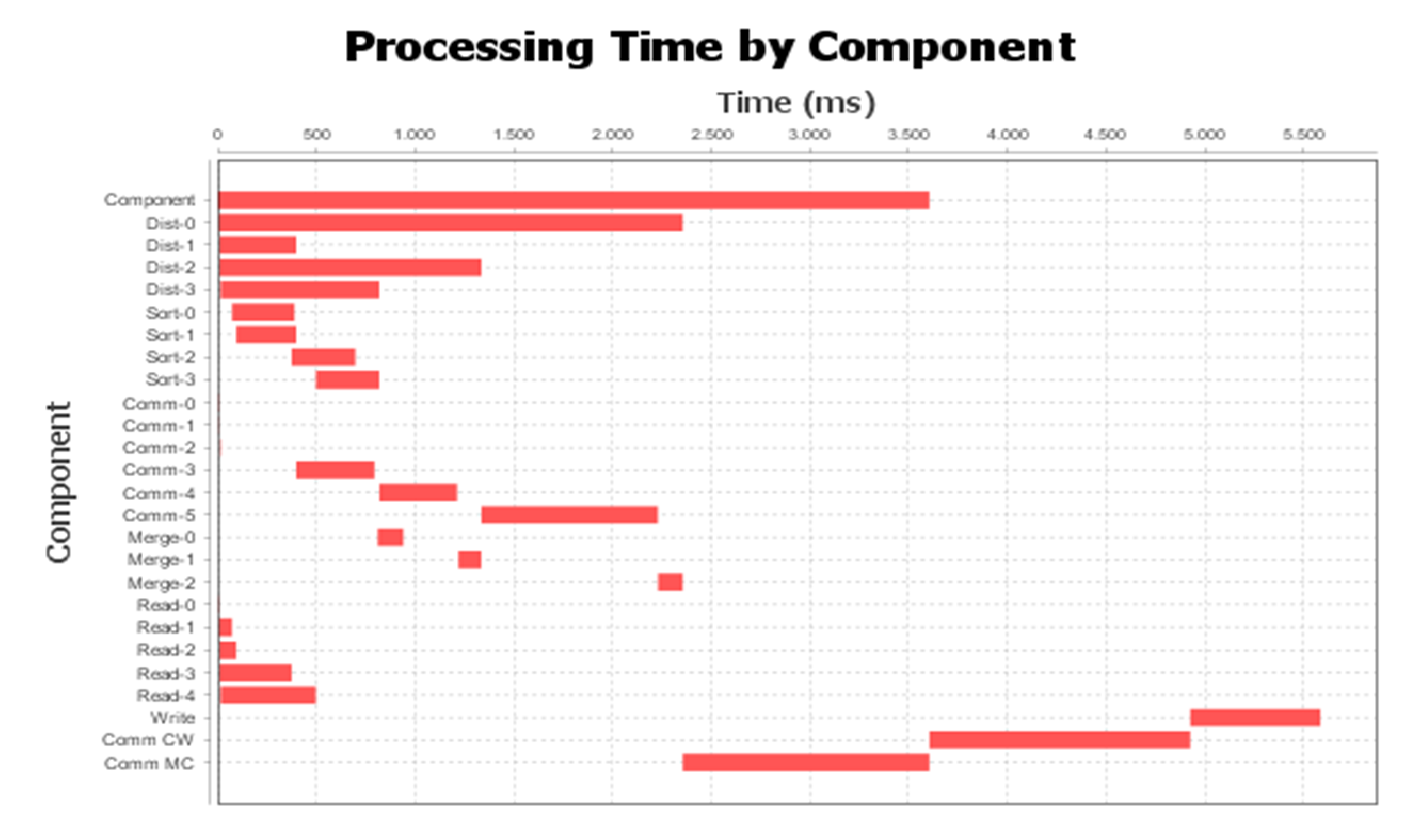
\includegraphics[trim=0.5cm 0cm -5cm 0cm, scale=0.74]{fig/JCUmaRmi498Behavior.eps}
	\caption{Behavior of the JC Sorting Strategy (UMA-RMI)}
	\label{fig:originalStrategyBehaviorRmi}
\end{figure}

First, figure \ref{fig:originalStrategyBehaviorRmi} corresponding to the experiment configured as: 
\begin{itemize}
	\item Communication protocol: RMI.
	\item  Memory structure: Uma.
	\item The number of available nodes: 4
	\item File size: 9'800.0000 Lines.
\end{itemize}
	
Figure \ref{fig:originalStrategyBehaviorRmi} allows to observe how the components interact during their execution (parallel and sequential processes), that is, their behavior. For example, we see that the time described by the chart label "component" has implicit the time corresponding to other components like sorters, mergers, distributors, except the communication time between the Control and the Writer and the writer time, because these components are executed later. The chart allows looking that the distribution phase is executed 4 times (components Dist 0 to Dist 4), one by each processing node. Additionally, we too can observe that the main distributor component-time (Dist 0) has implicit the time corresponding to other components, except the communication time between the merger and the Control components. In the same way figures \ref{fig:originalStrategyBehaviorRest} and \ref{fig:originalStrategyBehaviorIce} show the behavior of this pattern in different configurations.
	
\begin{figure}[H]
	\centering
	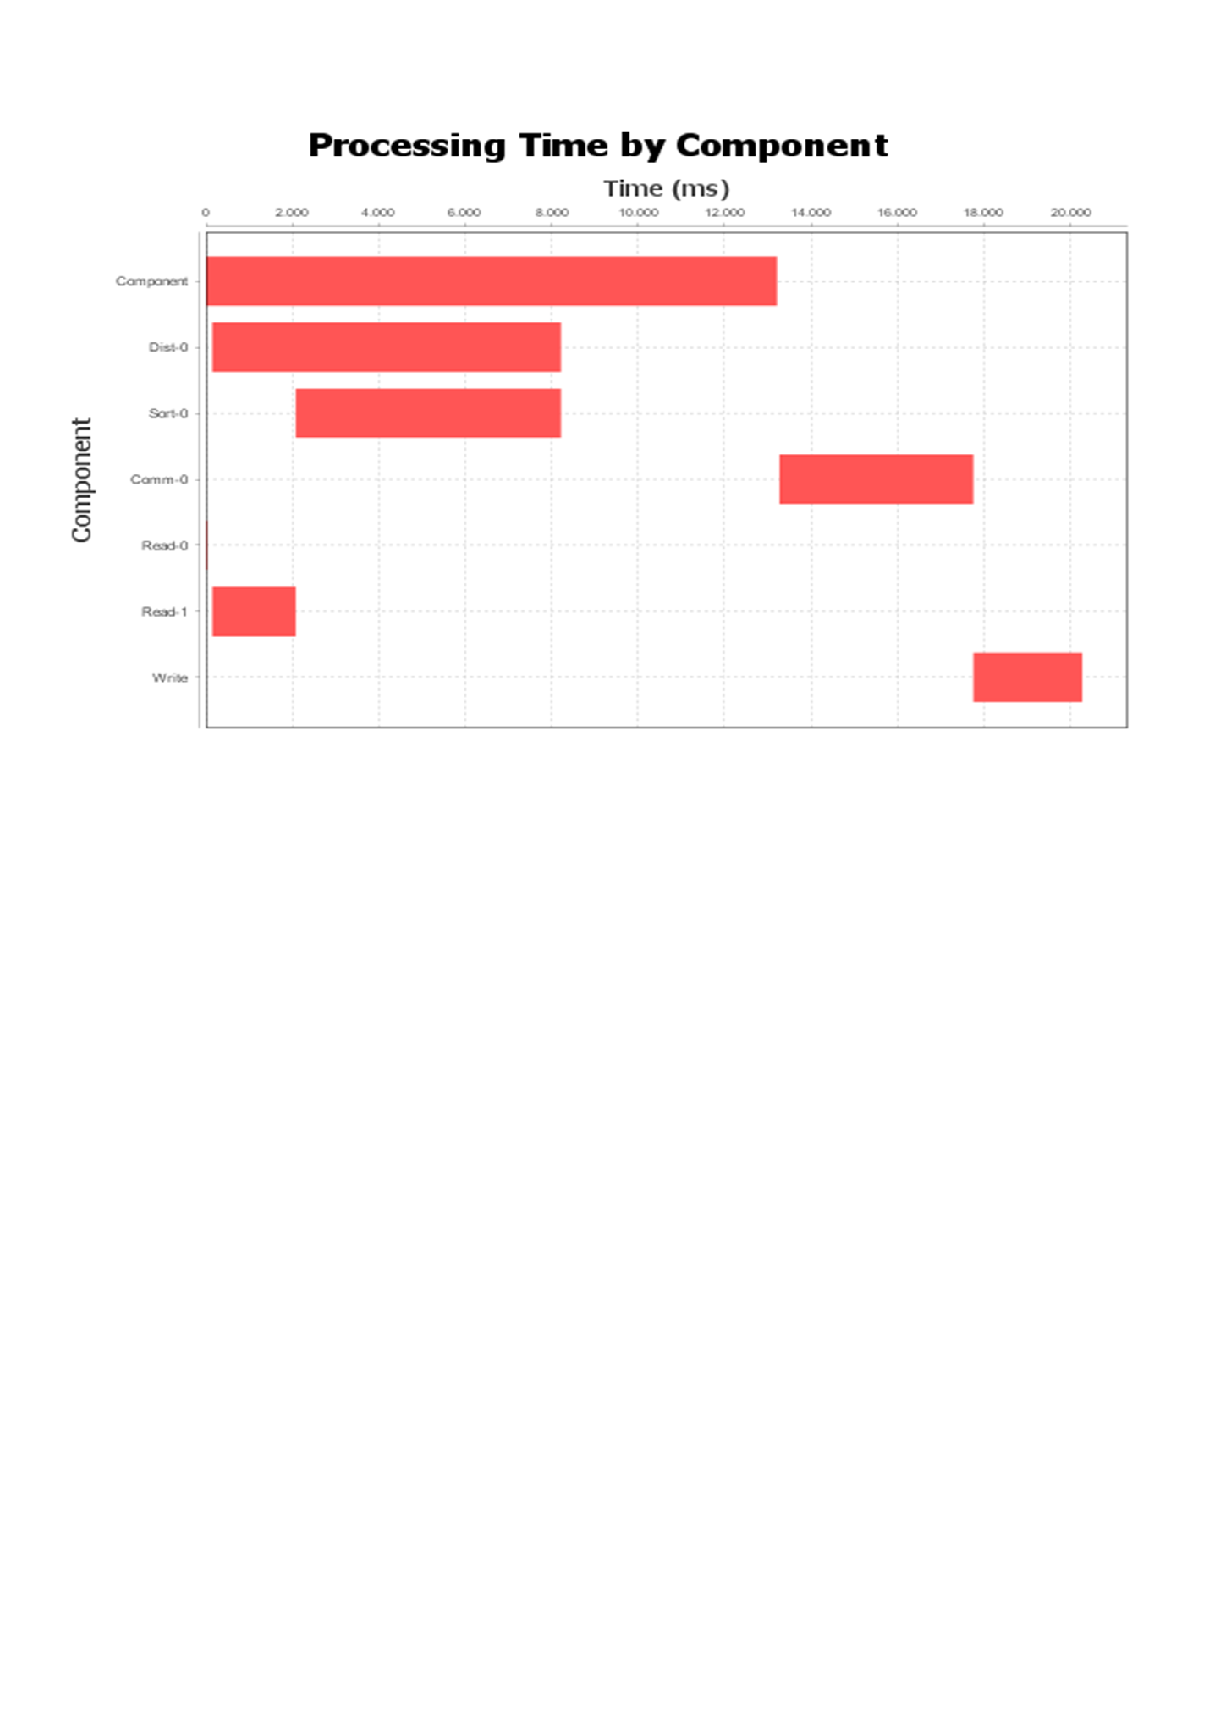
\includegraphics[trim=0.5cm 17cm -5cm 1cm, scale=0.9]{fig/JCUmaRest190Behavior.eps}
	\caption{Behavior of the JC Sorting Strategy (UMA-REST)}
	\label{fig:originalStrategyBehaviorRest}
\end{figure}

Second, figure \ref{fig:originalStrategyBehaviorRest} corresponding to the experiment configured as: 
\begin{itemize}
	\item Communication protocol: REST.
	\item  Memory structure: Uma.
	\item The number of available nodes: 1
 	\item File size: 9'000.0000 Lines.
\end{itemize}

\begin{figure}[H]
	\centering
	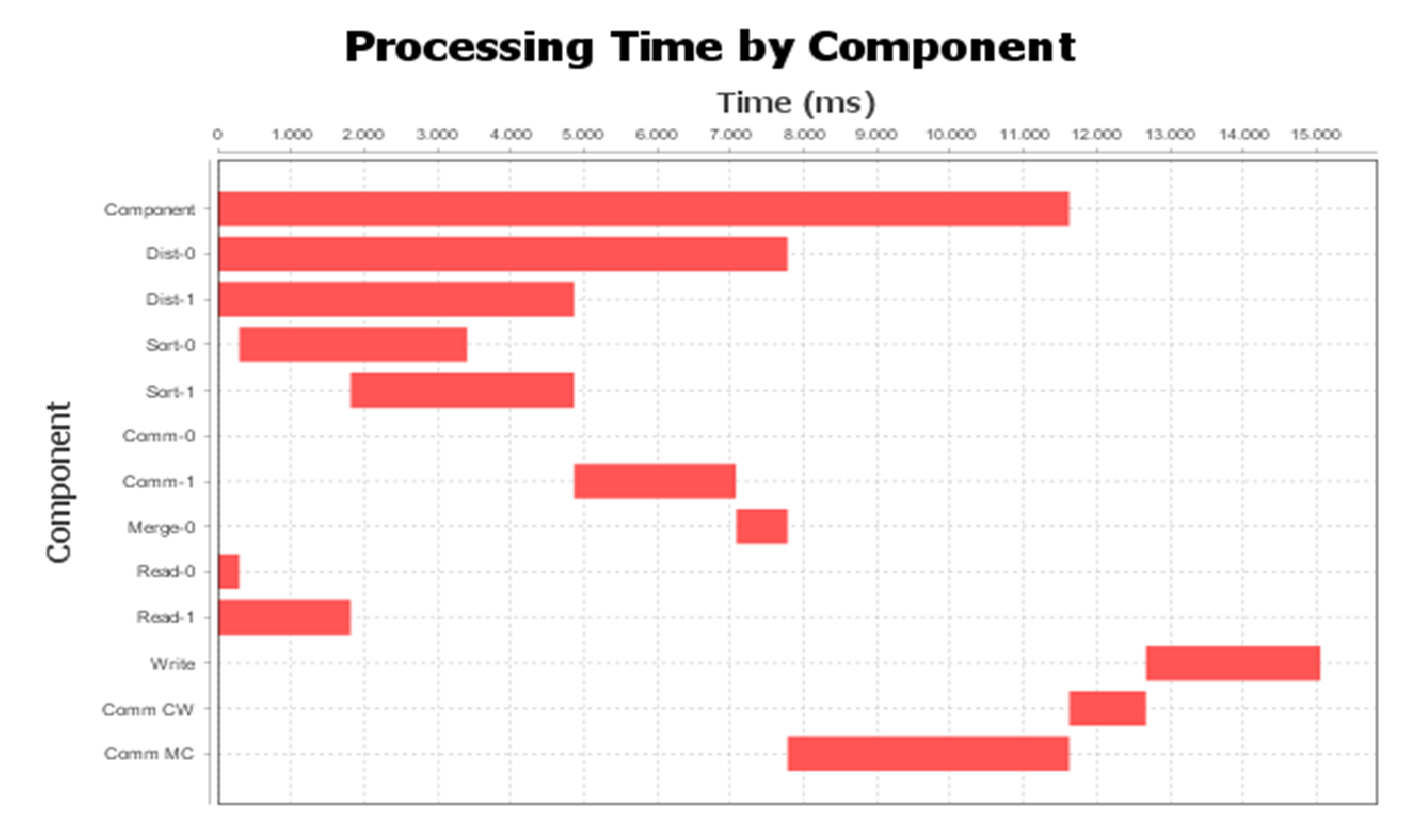
\includegraphics[trim=0.5cm 0cm -5cm 0cm, scale=0.74]{fig/JCUmaIce226Behavior.eps}
	\caption{Behavior of the JC Sorting Strategy (UMA-ICE)}
	\label{fig:originalStrategyBehaviorIce}
\end{figure}

Third, figure \ref{fig:originalStrategyBehaviorIce} corresponding to the experiment configured as: 
\begin{itemize}
	\item Communication protocol: ICE.
	\item  Memory structure: Uma.
	\item The number of available nodes: 2
	\item File size: 2'600.0000 Lines.
\end{itemize}

Throughout all configurations of the JC sorting strategy, we observe that the distribution phase of the main distributor includes, (i) the read phase time, (ii) the sort phase time, (iii) the merge phase time, and (iv) the communication phase time (i.e., the communication time among the distribution components). This is caused because each distributor that makes distribution must wait until all file parts that it distributed returned to it (already sorted) and it can merge them.

The communication phase time above mentioned does not include the communication time between the first distributor and the control component when the sorted file is returned to the control component. Additionally, the communication time between the control component and the writer component when the sorted file is sent to be written is neither included. These times and the communication among the distribution components to return the sorted file to be merged take a huge part of the total time because in the UMA configuration these are the communications with more data traveling through the network.

A particularity of the configuration with 1 available node is that the only one node is responsible to sort the whole file, therefore there is not a merge phase.
\subsection{Analysis of the Behavior of the JC Sorting Strategy Variation }

Figures \ref{fig:variationOriginalStrategyBehaviorIce}, \ref{fig:variationOriginalStrategyBehaviorRest}, and \ref{fig:variationOriginalStrategyBehaviorRmi} show the JC Sorting Strategy variation behavior on different configurations. 

Same that the JC Sorting Strategy, figures \ref{fig:variationOriginalStrategyBehaviorIce}, \ref{fig:variationOriginalStrategyBehaviorRest}, and \ref{fig:variationOriginalStrategyBehaviorRmi} show interaction among components during experiments execution in different configurations. This variation behaves (i.e., the interaction among components and time used by each component) different from the previous due to two main reasons, (i) the merge phase time is not included in the distribution phase time and (ii) the waiting time for the merge is introduced.

\begin{figure}[H]
	\centering
	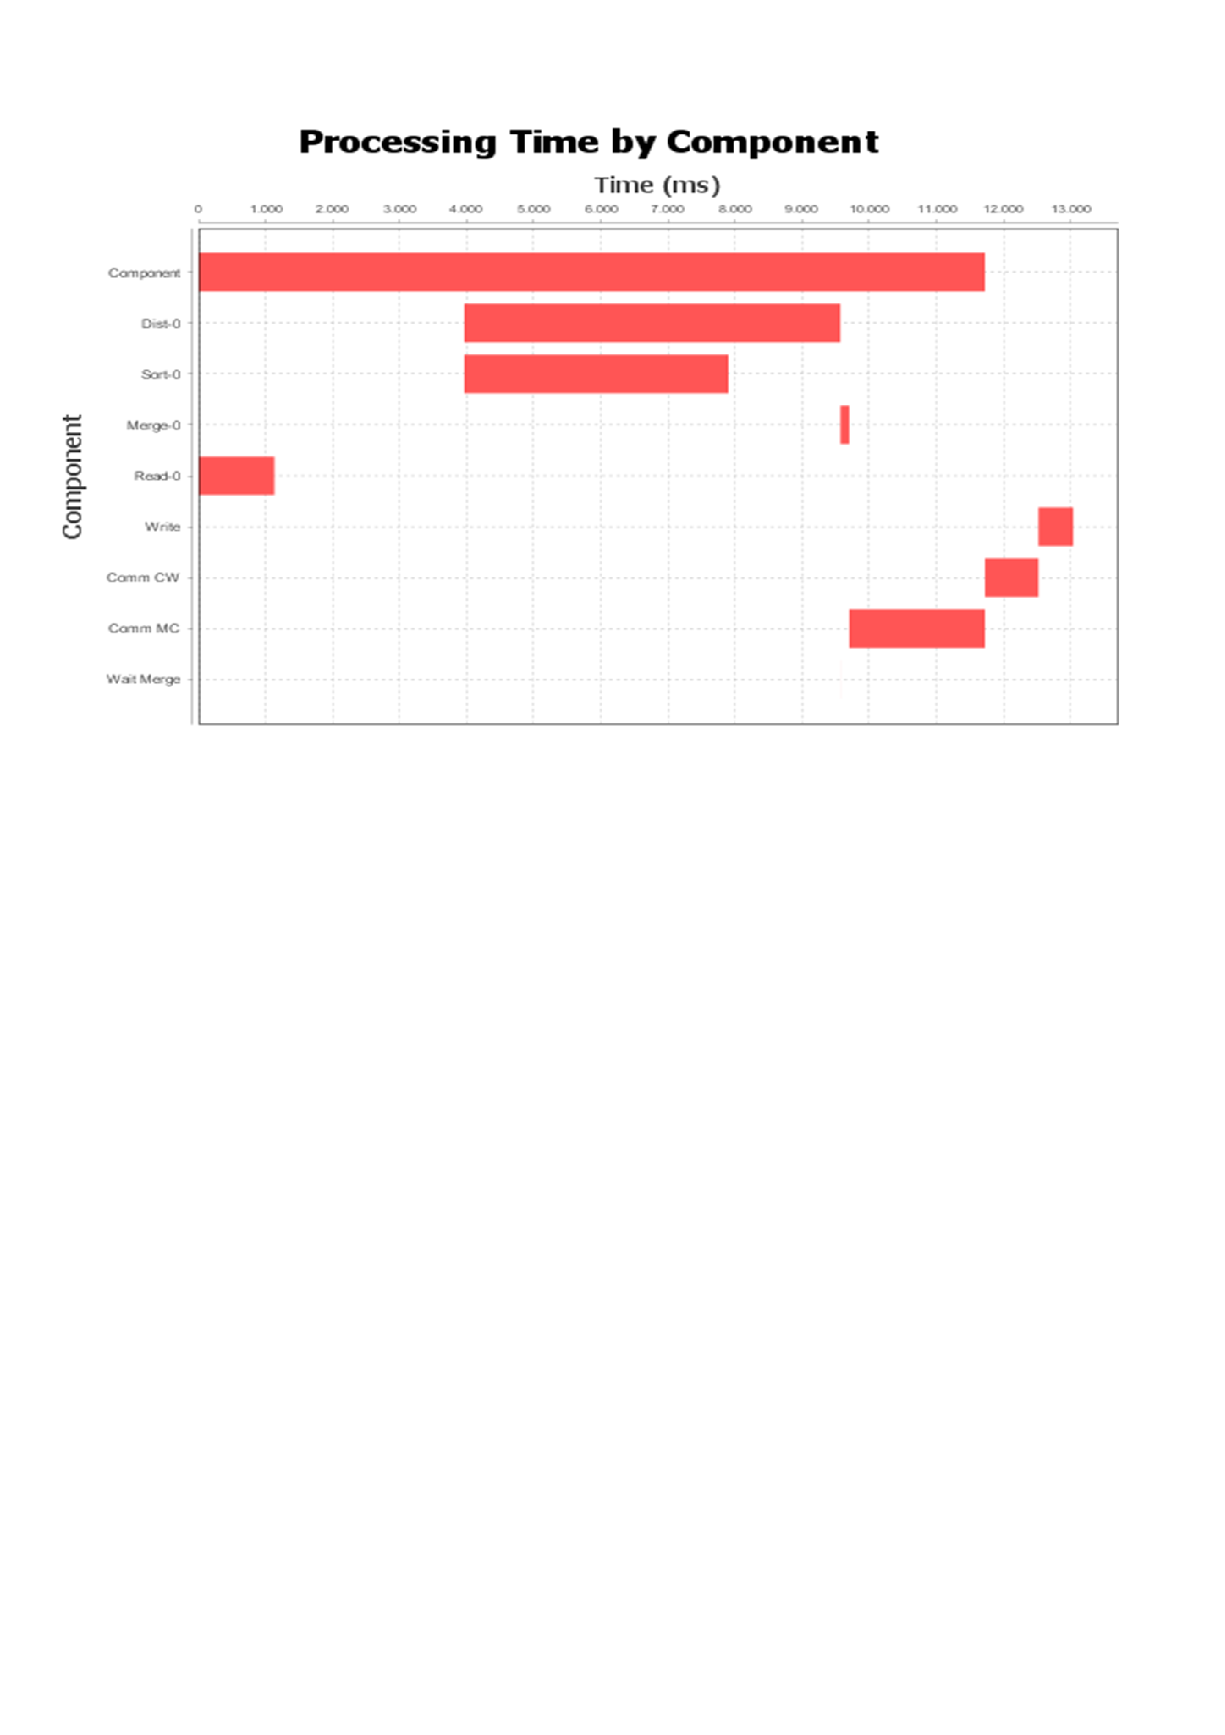
\includegraphics[trim=0.5cm 17cm -5cm 1cm, scale=0.9]{fig/MSNormaIce162Behavior.eps}
	\caption{Behavior of the JC Sorting Strategy Variation (NORMA-ICE)}
	\label{fig:variationOriginalStrategyBehaviorIce}
\end{figure}

First, figure \ref{fig:variationOriginalStrategyBehaviorIce} corresponding to the experiment configured as: 
\begin{itemize}
	\item Communication protocol: ICE.
	\item  Memory structure: Norma.
	\item The number of available nodes: 1
	\item File size: 6'200.0000 Lines.
\end{itemize}

\begin{figure}[H]
	\centering
	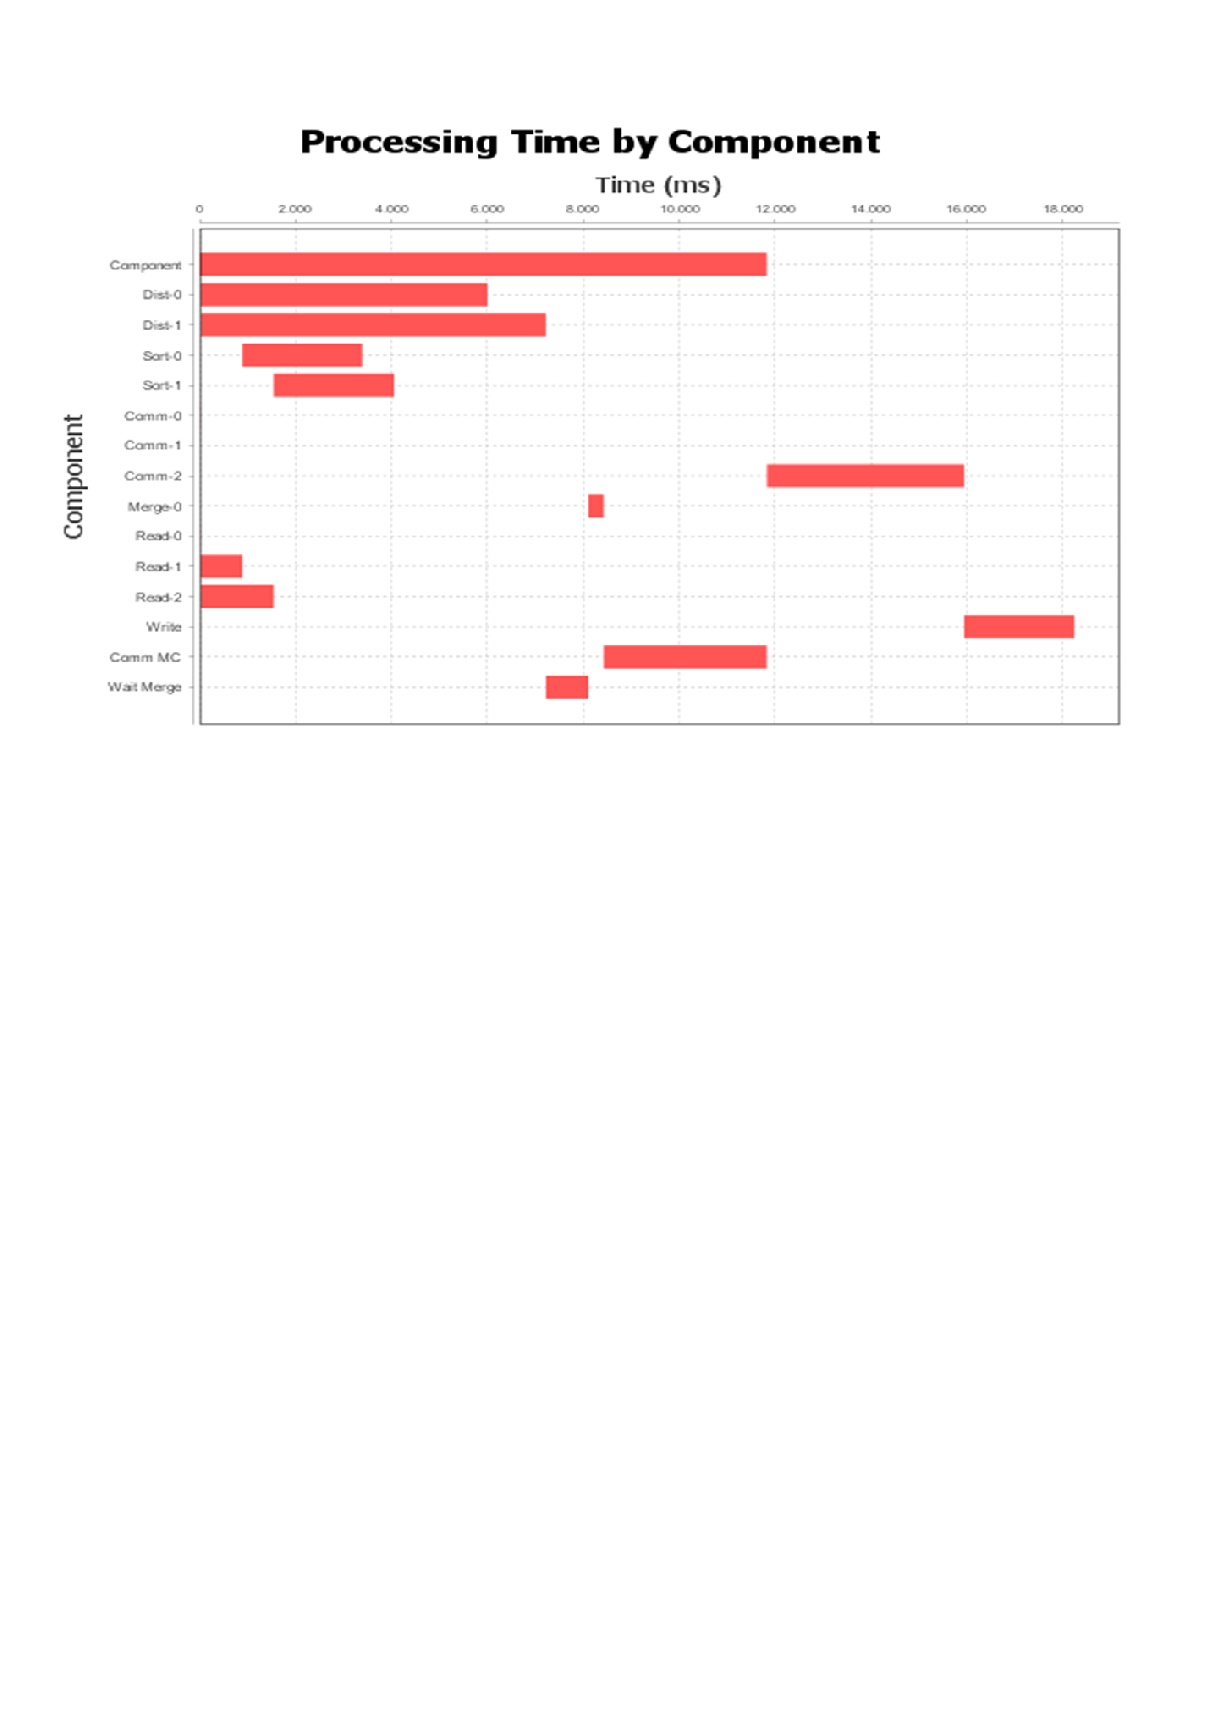
\includegraphics[trim=0.5cm 17cm -5cm 1cm, scale=0.9]{fig/MSUmaRest282Behavior.eps}
	\caption{Behavior of the JC Sorting Strategy Variation (UMA-REST)}
	\label{fig:variationOriginalStrategyBehaviorRest}
\end{figure}

Second,figure \ref{fig:variationOriginalStrategyBehaviorRest} corresponding to the experiment configured as: 
\begin{itemize}
	\item Communication protocol: REST.
	\item  Memory structure: Uma.
	\item The number of available nodes: 2
	\item File size: 8'200.0000 Lines.
\end{itemize}

\begin{figure}[H]
	\centering
	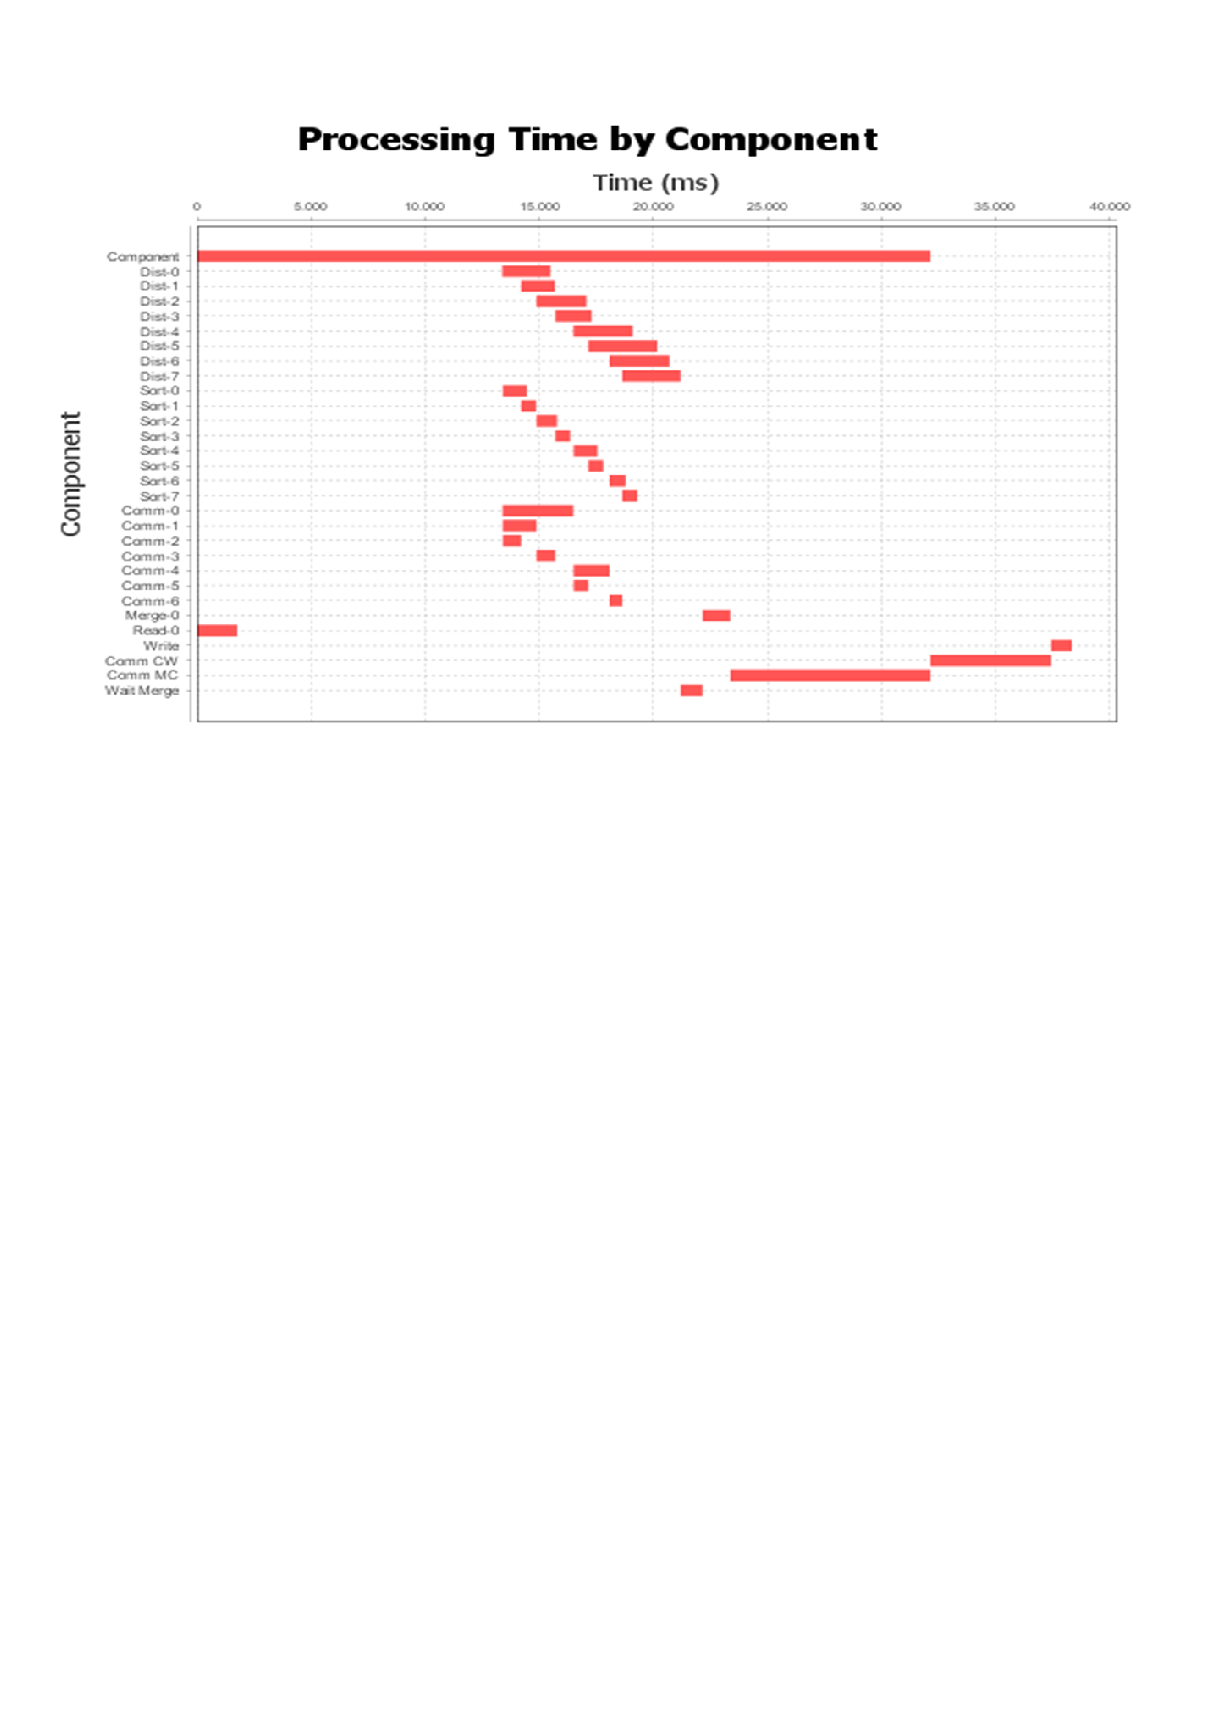
\includegraphics[trim=0.5cm 17cm -5cm 1cm, scale=0.9]{fig/MSNormaRmi890Behavior.eps}
	\caption{Behavior of the JC Sorting Strategy Variation (NORMA-RMI)}
	\label{fig:variationOriginalStrategyBehaviorRmi}
\end{figure}

Third, figure \ref{fig:variationOriginalStrategyBehaviorRmi} corresponding to the experiment configured as: 
\begin{itemize}
	\item Communication protocol: RMI.
	\item  Memory structure: Norma.
	\item The number of available nodes: 8
	\item File size: 9'000.0000 Lines.
\end{itemize}


The NORMA configurations show a time that was not measured in the first experiments, this can be observed in figures \ref{fig:variationOriginalStrategyBehaviorIce} and \ref{fig:variationOriginalStrategyBehaviorRmi}. These figures show that between the read component measured time and the first distributor component measured time, there is a considerable time that was unknown its source. In posterior experiments, new measures were introduced and then we discover that the unknown time corresponds to the communication time between the read component and the control component when the file to be sorted is read and loaded to memory. In addition, the communication time when the control component sends the read file to the main distributor. These measures suggest that despite the components are located in the same node, the communication time among these components is not depreciable.

Another time that was not measured is the time to send the sorted file part from the sort component to the merge component, this time can be observed as the time from end the sort phase time until the end of the distribution phase time. 

Because the file to be sorted should travel from one component to other, therefore, we conclude that when we are in a distributed environment an important key is to keep the communication time as small as to be possibly among processing nodes and among components in the same processing node too.

%\newpage

\subsection{Analysis of the Behavior of the Fork/Join Java Library Variation }

The figures \ref{fig:forkJoinLibraryBehaviorIce}, \ref{fig:forkJoinLibraryBehaviorRest}, and \ref{fig:forkJoinLibraryBehaviorRmi} show the Fork/Join Java library variation behavior on different configurations. 

\begin{figure}[H]
	\centering
	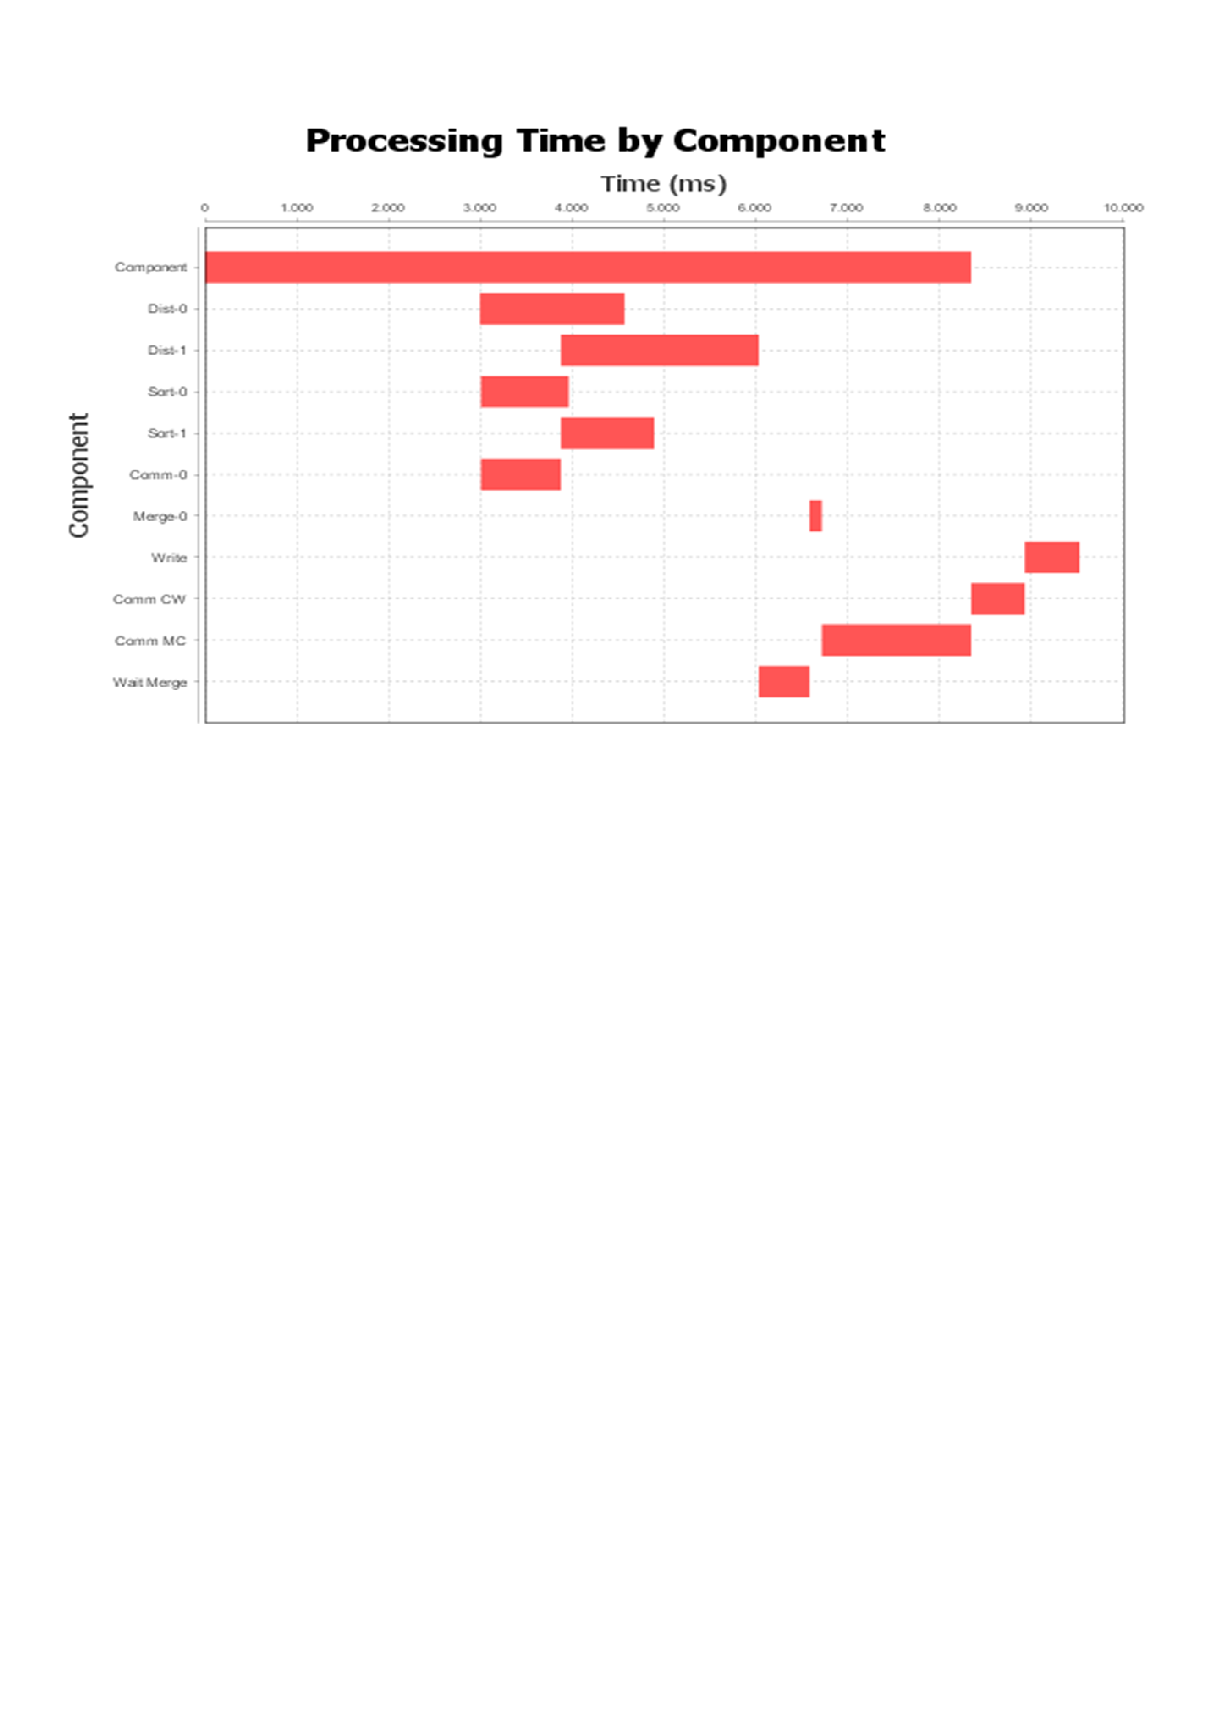
\includegraphics[trim=0.5cm 17cm -5cm 1cm, scale=0.9]{fig/FJNormaIce250Behavior.eps}
	\caption{Behavior of the Fork/Join Java Library Variation (NORMA-ICE)}
	\label{fig:forkJoinLibraryBehaviorIce}
\end{figure}
First, figure \ref{fig:forkJoinLibraryBehaviorIce} corresponding to the experiment configured as: 
\begin{itemize}
	\item Communication protocol: ICE.
	\item  Memory structure: Norma.
	\item The number of available nodes: 2
	\item File size: 5'000.0000 Lines.
\end{itemize}

\begin{figure}[H]
	\centering
	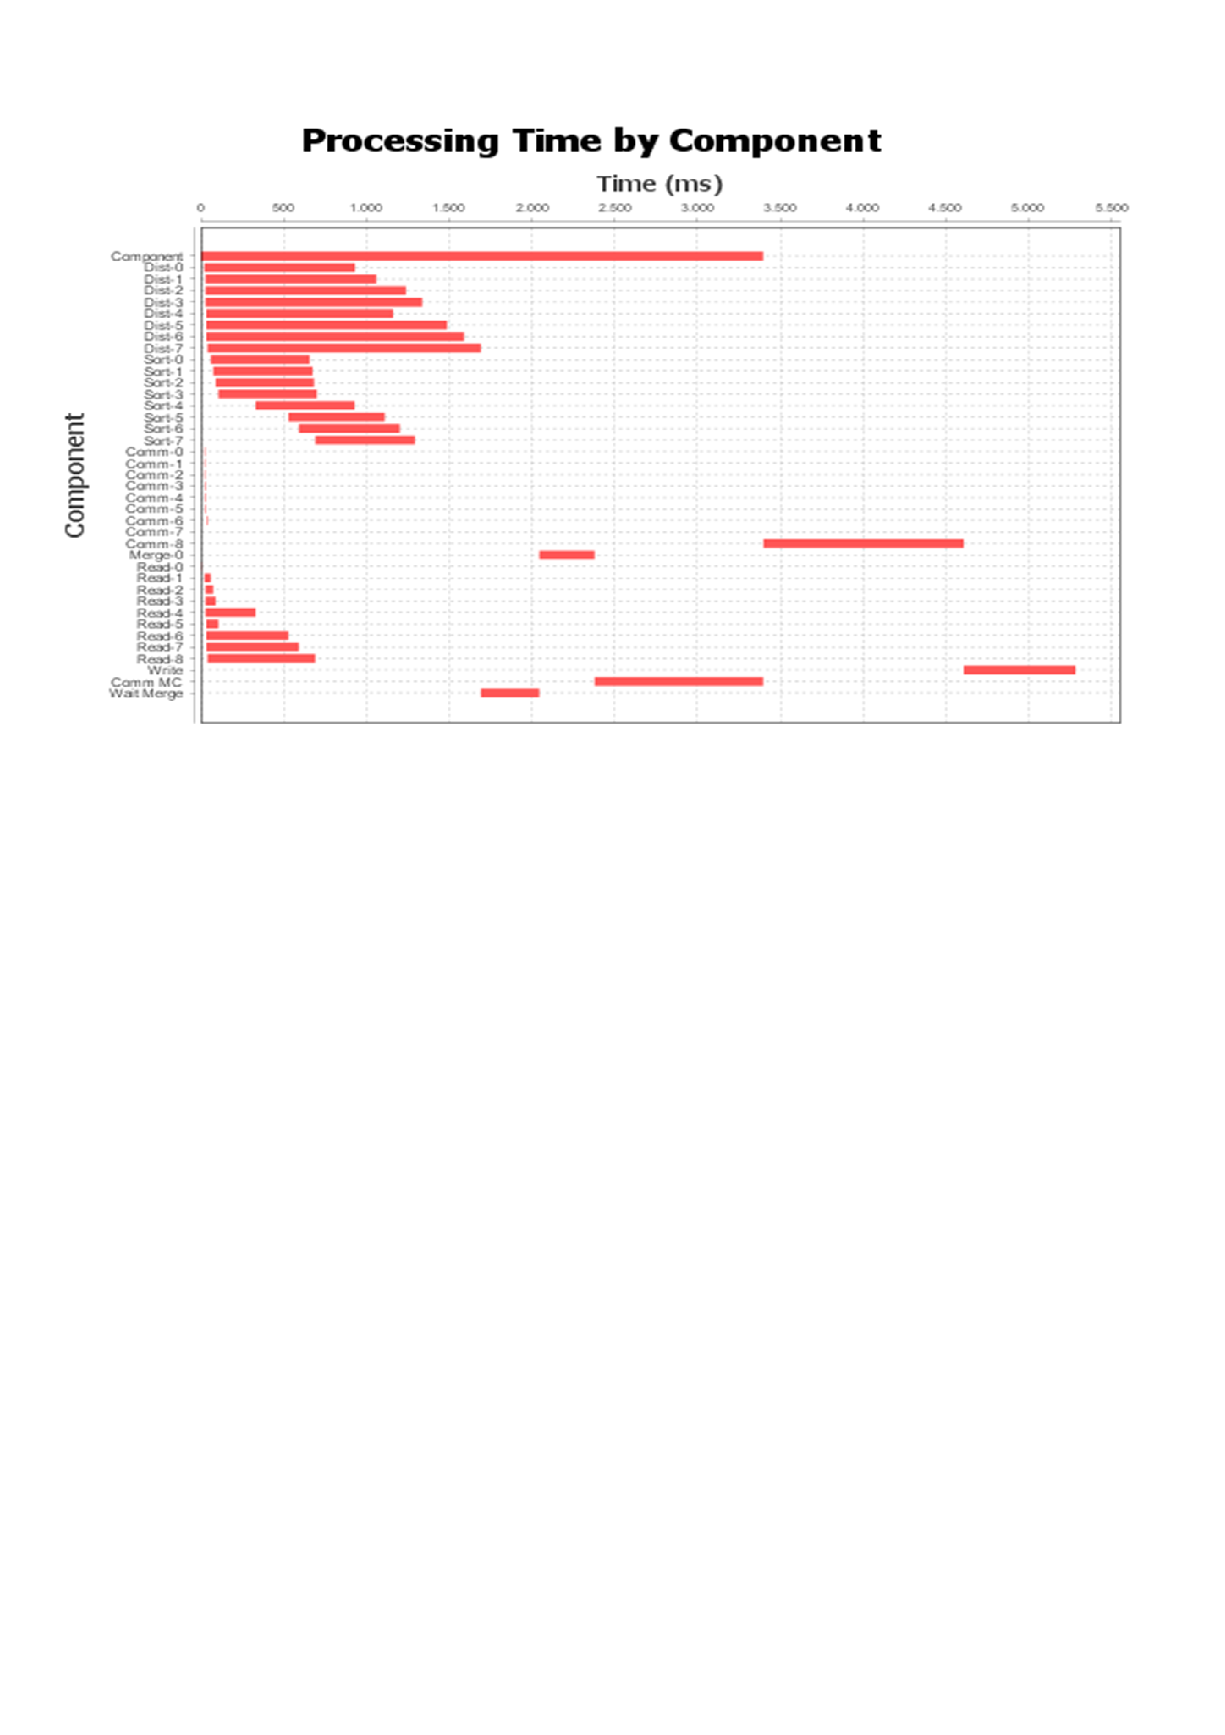
\includegraphics[trim=0.5cm 17cm -5cm 1cm, scale=0.9]{fig/FJUmaRest826Behavior.eps}
	\caption{Behavior of the Fork/Join Java Library Variation (UMA-REST)}
	\label{fig:forkJoinLibraryBehaviorRest}
\end{figure}
Second, figure \ref{fig:forkJoinLibraryBehaviorRest} corresponding to the experiment configured as: 
\begin{itemize}
	\item Communication protocol: REST.
	\item  Memory structure: Uma.
	\item The number of available nodes: 8
	\item File size: 2'600.0000 Lines.
\end{itemize}

In UMA configurations the distribution phase includes the read and sort phases, first, the read phase is executed and then the sort phase can be executed. We can observe that the read phase has specific behavior with UMA, all distribution and read phases start almost at the same time, however, despite each reading phase reads the same size of different file parts, each read can take a different time amount. This situation shows the UMA limitations when many components try to access the memory, we can observe in figures \ref{fig:variationOriginalStrategyBehaviorRest} and \ref{fig:forkJoinLibraryBehaviorRest} that between more read phases, the time to read the same file size has more variation. This causes that the sort phase starts at different times and each distribution phase uses a different amount of time to sort the different file parts with the same size.

\begin{figure}[H]
	\centering
	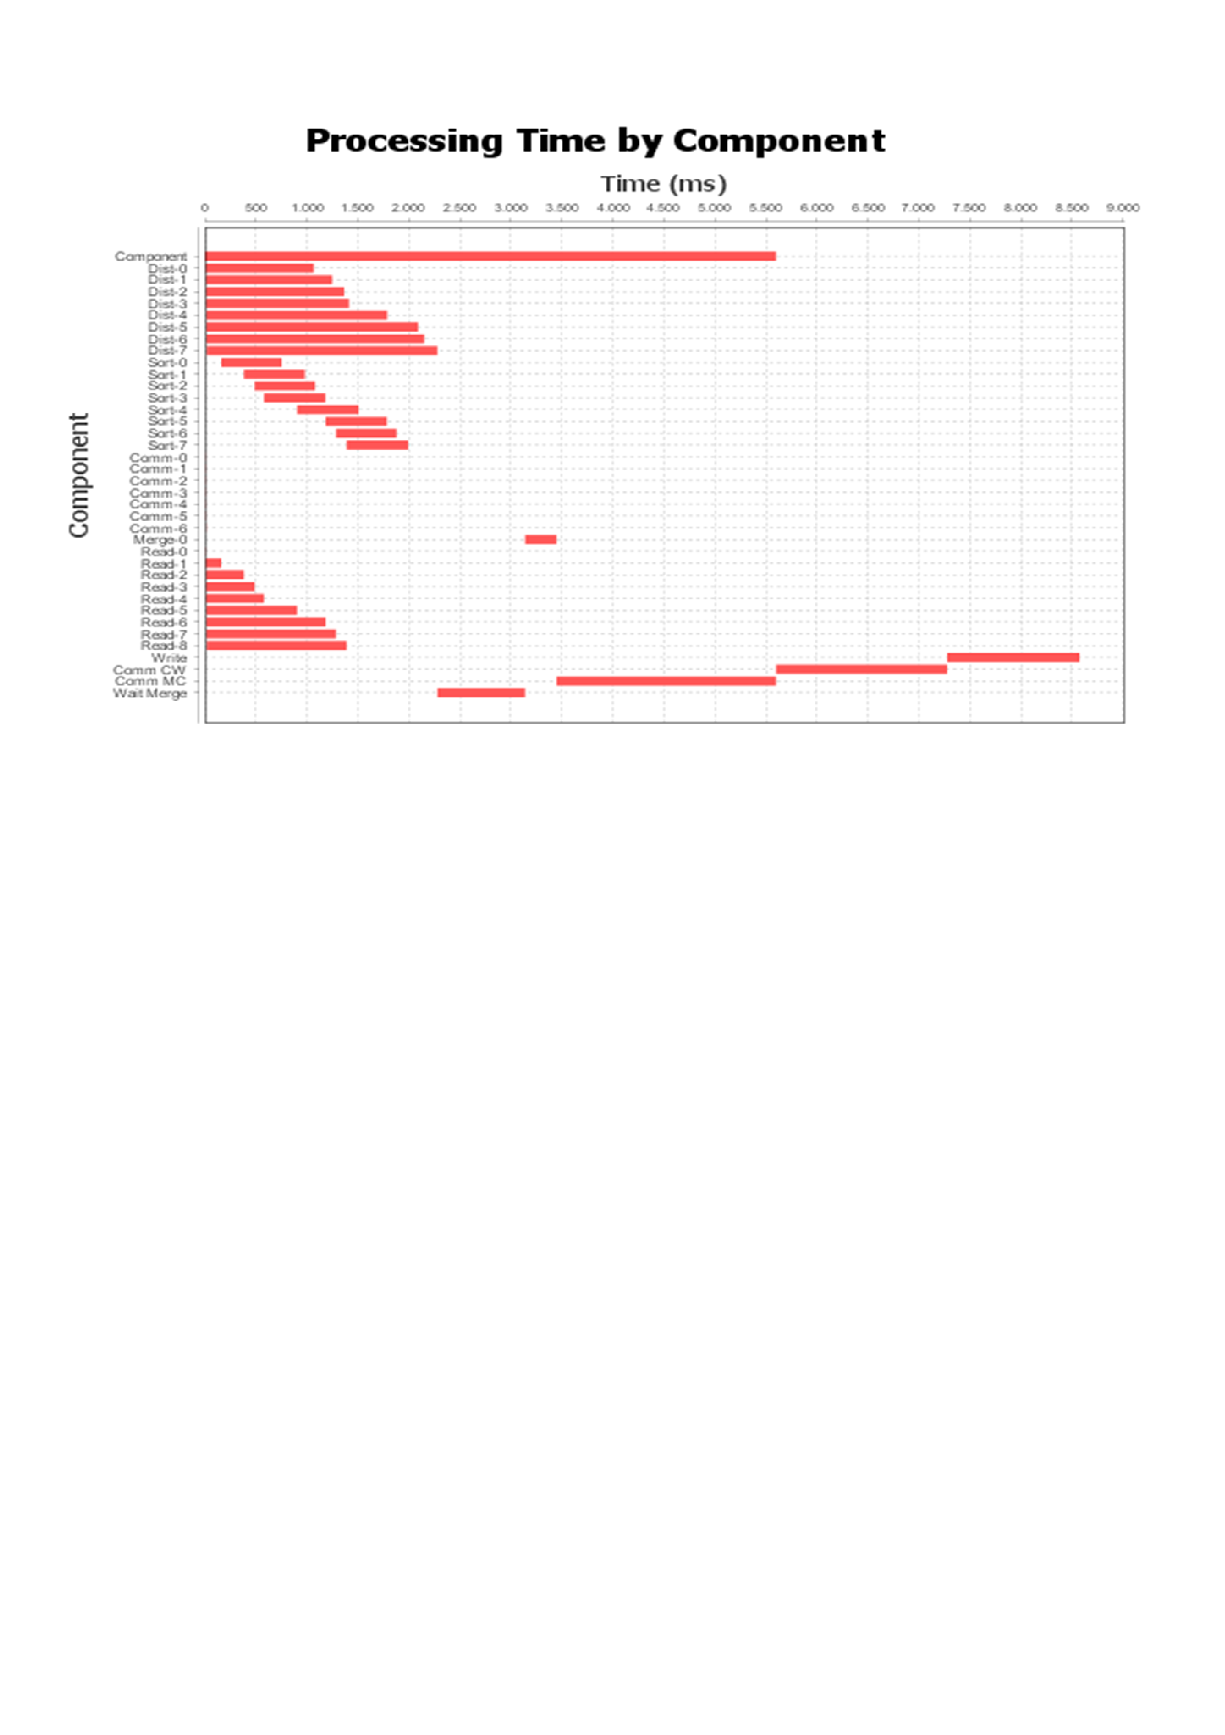
\includegraphics[trim=0.5cm 17cm -5cm 1cm, scale=0.9]{fig/FJUmaRmi842Behavior.eps}
	\caption{Behavior of the Fork/Join Java Library Variation (UMA-RMI)}
	\label{fig:forkJoinLibraryBehaviorRmi}
\end{figure}
Third,figure \ref{fig:forkJoinLibraryBehaviorRmi} corresponding to the experiment configured as: 
\begin{itemize}
	\item Communication protocol: RMI.
	\item  Memory structure: Uma.
	\item The number of available nodes: 8
	\item File size: 4'200.0000 Lines.
\end{itemize}

This variation has the same behavior as the JC Sorting Strategy variation, that is, the changes in the behavior is not observed through the figures \ref{fig:forkJoinLibraryBehaviorIce}, \ref{fig:forkJoinLibraryBehaviorRest}, and \ref{fig:forkJoinLibraryBehaviorRmi}, because the main change is in how the CPU cores are used. Including the interaction among components in the NORMA and UMA configurations. Each sort phase uses the fork / join Java library. To use this library implies to determine a threshold until the item to be processed is forked. We define the threshold according to the CPU use percentage of each node's CPUs and the part file to be sorted. If the CPU use percentage of one CPU core is less than 40\%, it is a candidate to be used. However, the operating system is responsible for finally assigning work to each CPU core. The threshold was calculated as the part file length divided on the CPU core amount that could be used.

\subsection{Analysis of the Behavior of the Fork-Join Design Pattern }

Figures \ref{fig:forkJoinBehaviorIce}, \ref{fig:forkJoinBehaviorRest}, and \ref{fig:forkJoinBehaviorRmi} show the Fork/Join design pattern behavior on different configurations. 

\begin{figure}[H]
	\centering
	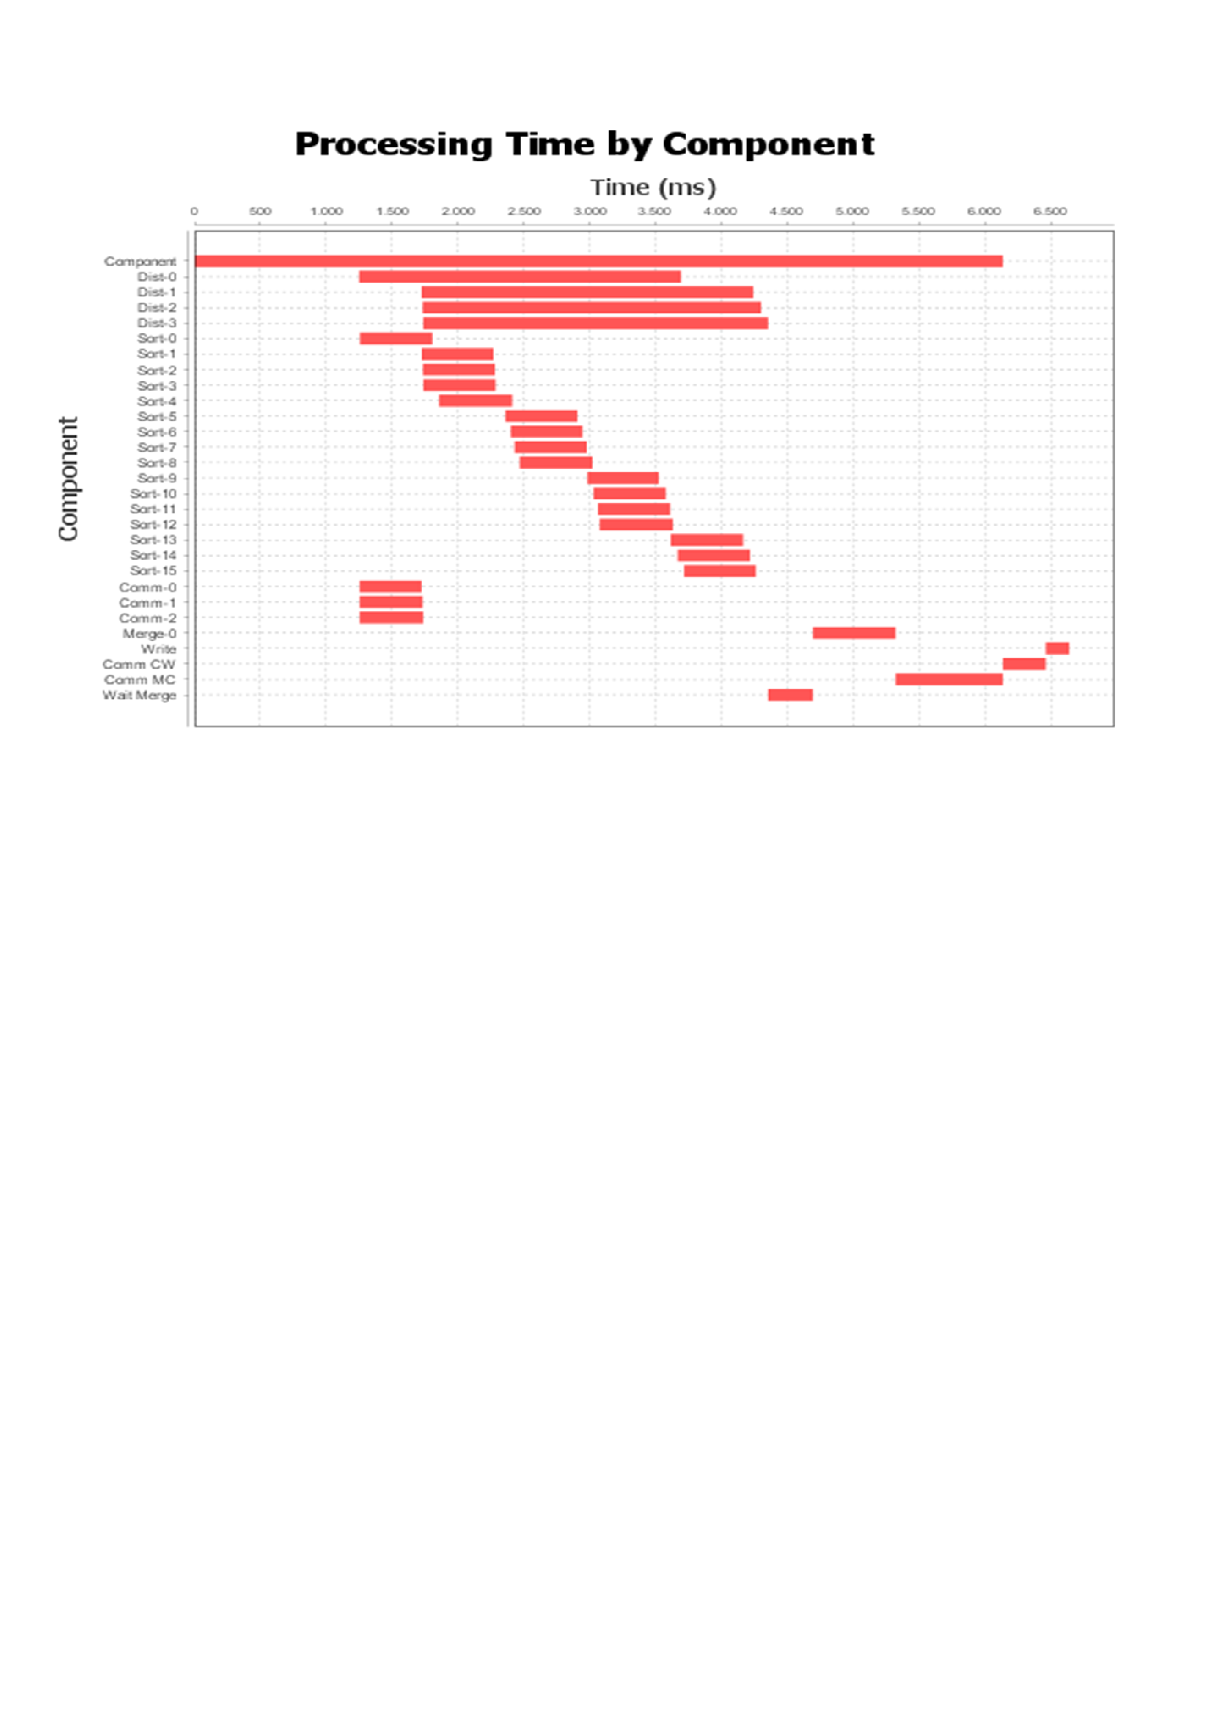
\includegraphics[trim=0.5cm 17cm -5cm 1cm, scale=0.9]{fig/FJDNormaIce426Behavior.eps}
	\caption{Behavior of the Fork-Join Design Pattern (NORMA-ICE)}
	\label{fig:forkJoinBehaviorIce}
\end{figure}

First, figure \ref{fig:forkJoinBehaviorIce} corresponding to the experiment configured as: 
\begin{itemize}
	\item Communication protocol: ICE.
	\item  Memory structure: Norma.
	\item The number of available nodes: 4
	\item File size: 2'600.0000 Lines.
\end{itemize}

This design pattern has a behavior very different from the above strategies, figure \ref{fig:forkJoinBehaviorIce} shows that there are only four distribution phases, one for each processing node, but there are 16 sort phases, four for each distribution phase. This behavior is caused by all processing nodes divides their own file part waiting that their children help to process if children finish processing before its parent. The times used to process in each processing node are very similar, unlike the above strategies.

\begin{figure}[H]
	\centering
	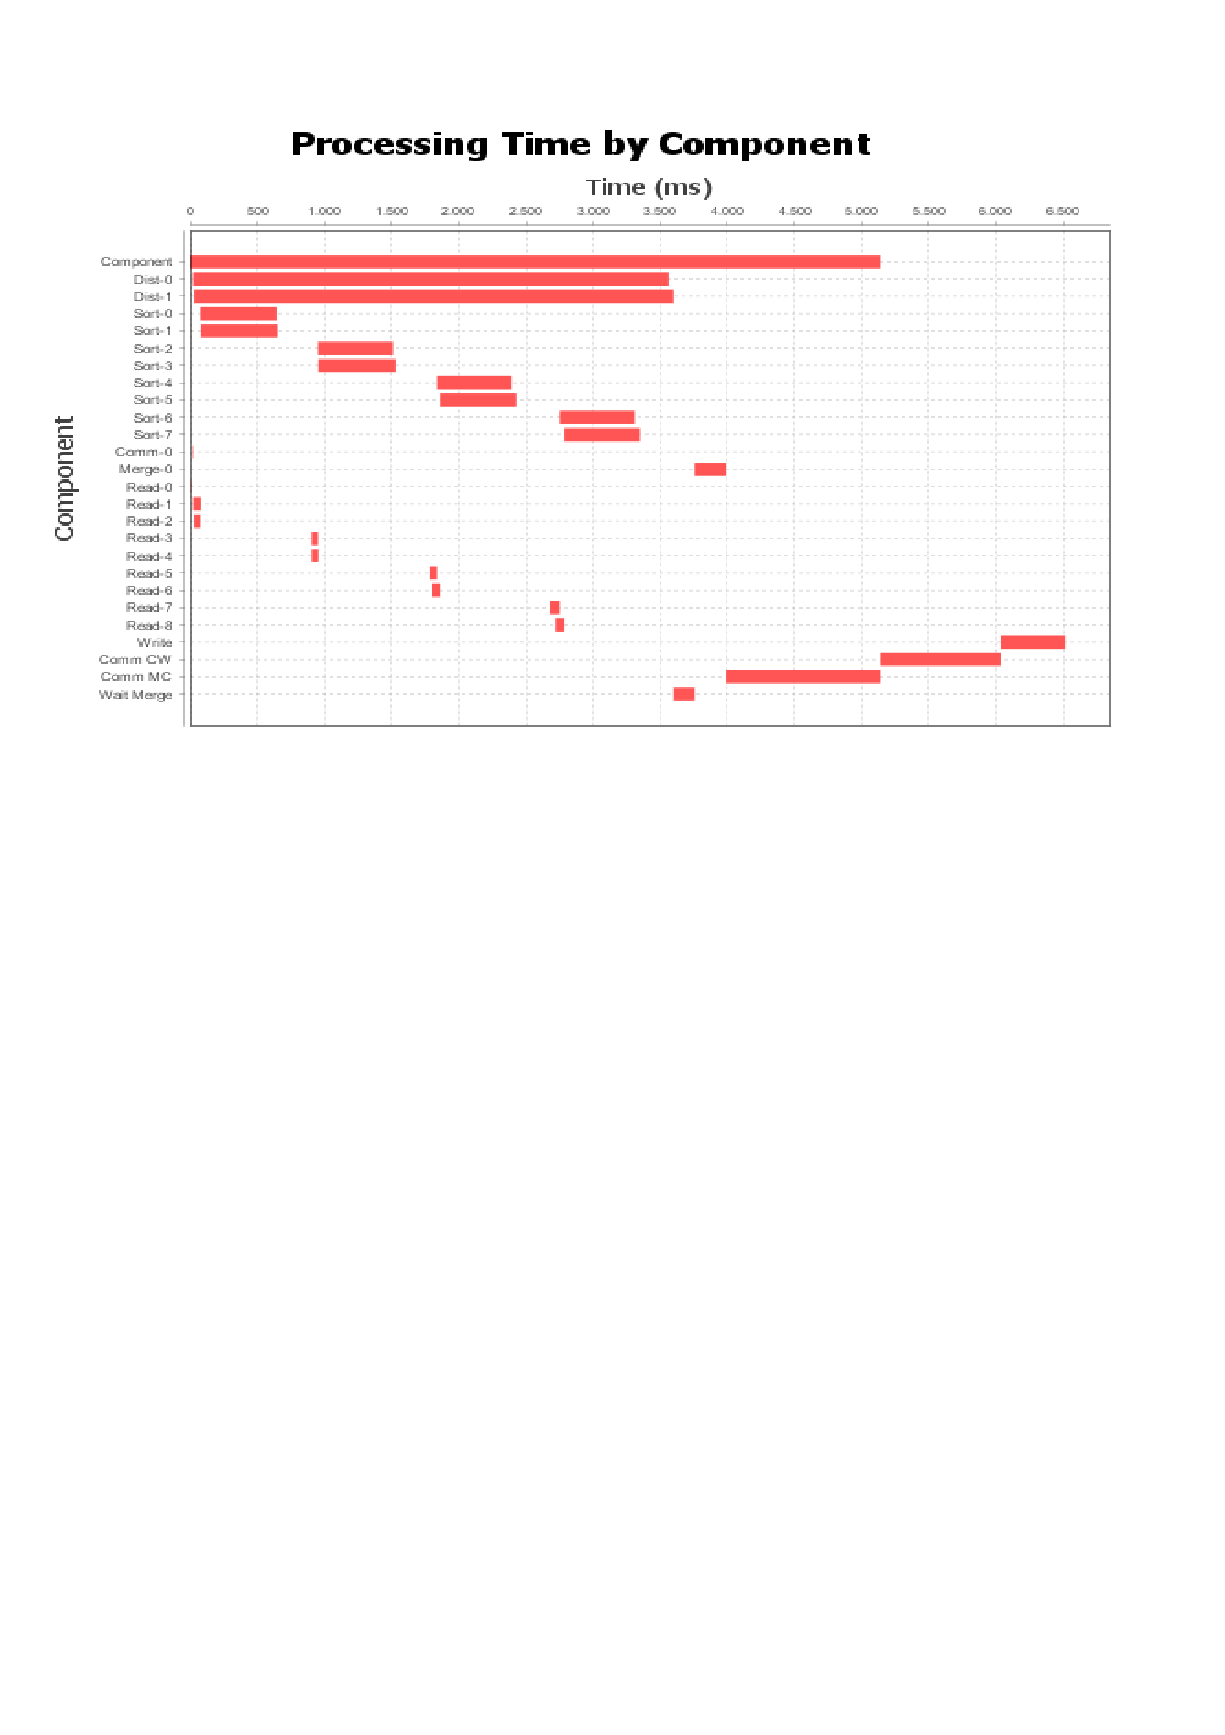
\includegraphics[trim=0.5cm 17cm -5cm 1cm, scale=0.9]{fig/FJDUmaRest218Behavior.eps}
	\caption{Behavior of the Fork-Join Design Pattern (UMA-REST)}
	\label{fig:forkJoinBehaviorRest}
\end{figure}
Second, figure \ref{fig:forkJoinBehaviorRest} corresponding to the experiment configured as: 
\begin{itemize}
	\item Communication protocol: REST.
	\item  Memory structure: Uma.
	\item The number of available nodes: 2
	\item File size: 1'800.0000 Lines.
\end{itemize}

This pattern shows the same behavior detected in the interaction among components in the NORMA and UMA configurations in above strategies.

\begin{figure}[H]
	\centering
	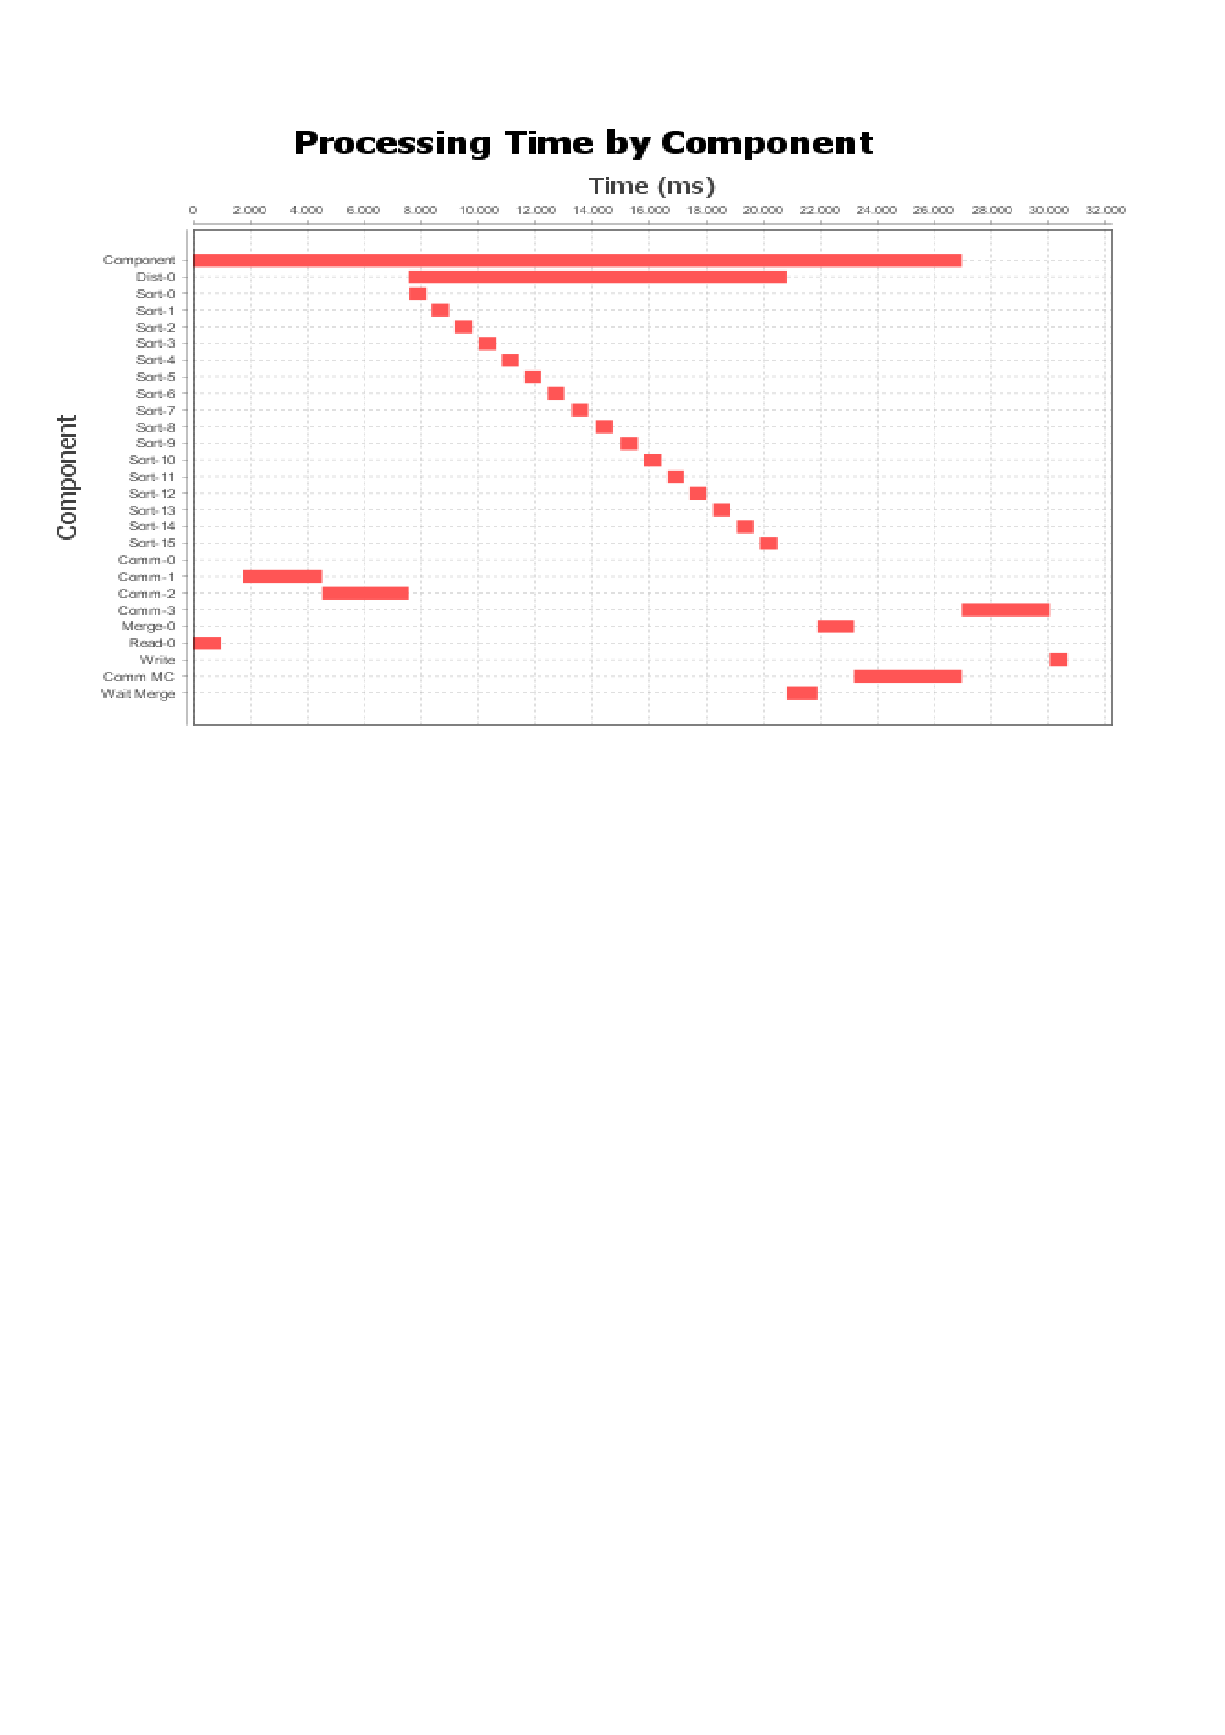
\includegraphics[trim=0.5cm 17cm -5cm 1cm, scale=0.9]{fig/FJDNormaRmi154Behavior.eps}
	\caption{Behavior of the Fork-Join Design Pattern (NORMA-RMI)}
	\label{fig:forkJoinBehaviorRmi}
\end{figure}
Third, figure \ref{fig:forkJoinBehaviorRmi} corresponding to the experiment configured as: 
\begin{itemize}
	\item Communication protocol: RMI.
	\item  Memory structure: Norma.
	\item The number of available nodes: 1
	\item File size: 5'400.0000 Lines.
\end{itemize}

In figure \ref{fig:forkJoinBehaviorRmi} we can observe that only one processing node is configured and 16 sort phases are executed the same that in figure \ref{fig:forkJoinBehaviorIce}, this is caused because the sort phases amount is not dependent of processing nodes amount, else it depends on the file size.

This design pattern tries to distribute in a homogeneous way, that is, all nodes can have the same nodes number of children. This is an important difference to the JC Sorting Strategy and it causes a completely different behavior. First, the file to be sorted is split considering not only the number available nodes but also the minimum file size to leverage distribution. The minimum file size was configured as 400.000 lines, as determined by preparatory experiments. 

Each node splits the file to be sorted and sends all parts (including its own part)  to be sorted at the same time. This is the first difference that we can observe between figures \ref{fig:forkJoinBehaviorIce} and \ref{fig:forkJoinBehaviorRest}. The time for the distribution phase is very similar at the same level, where a level represents how many processing nodes are located before hierarchically, for example, the first father is located in the "n" level and all its children are located in the "n-1" level. For example, in figure \ref{fig:forkJoinBehaviorIce}, Dist0 corresponding to a superior level, but Dist1, Dist2, and Dist3 are very similar given that they are at the same level.

The second difference is observed in the sort phase. Each node recursively divides its own file part into halves while the file part is bigger than the minimum file size to distribute and it sends each half to the queue. Then, each node sorts the file parts in the queue. The queue allows that if a child node finishes its processes before its father node, it can take work of the father queue. To sort each queue item, this variation uses the fork / join Java library.

This design pattern shows the same difference between the UMA and NORMA configurations detected in the JC Sorting Strategy Variation.

\subsection{Analysis of the Behavior of the Leader-Followers Design Pattern }

\begin{figure}[H]
	\centering
	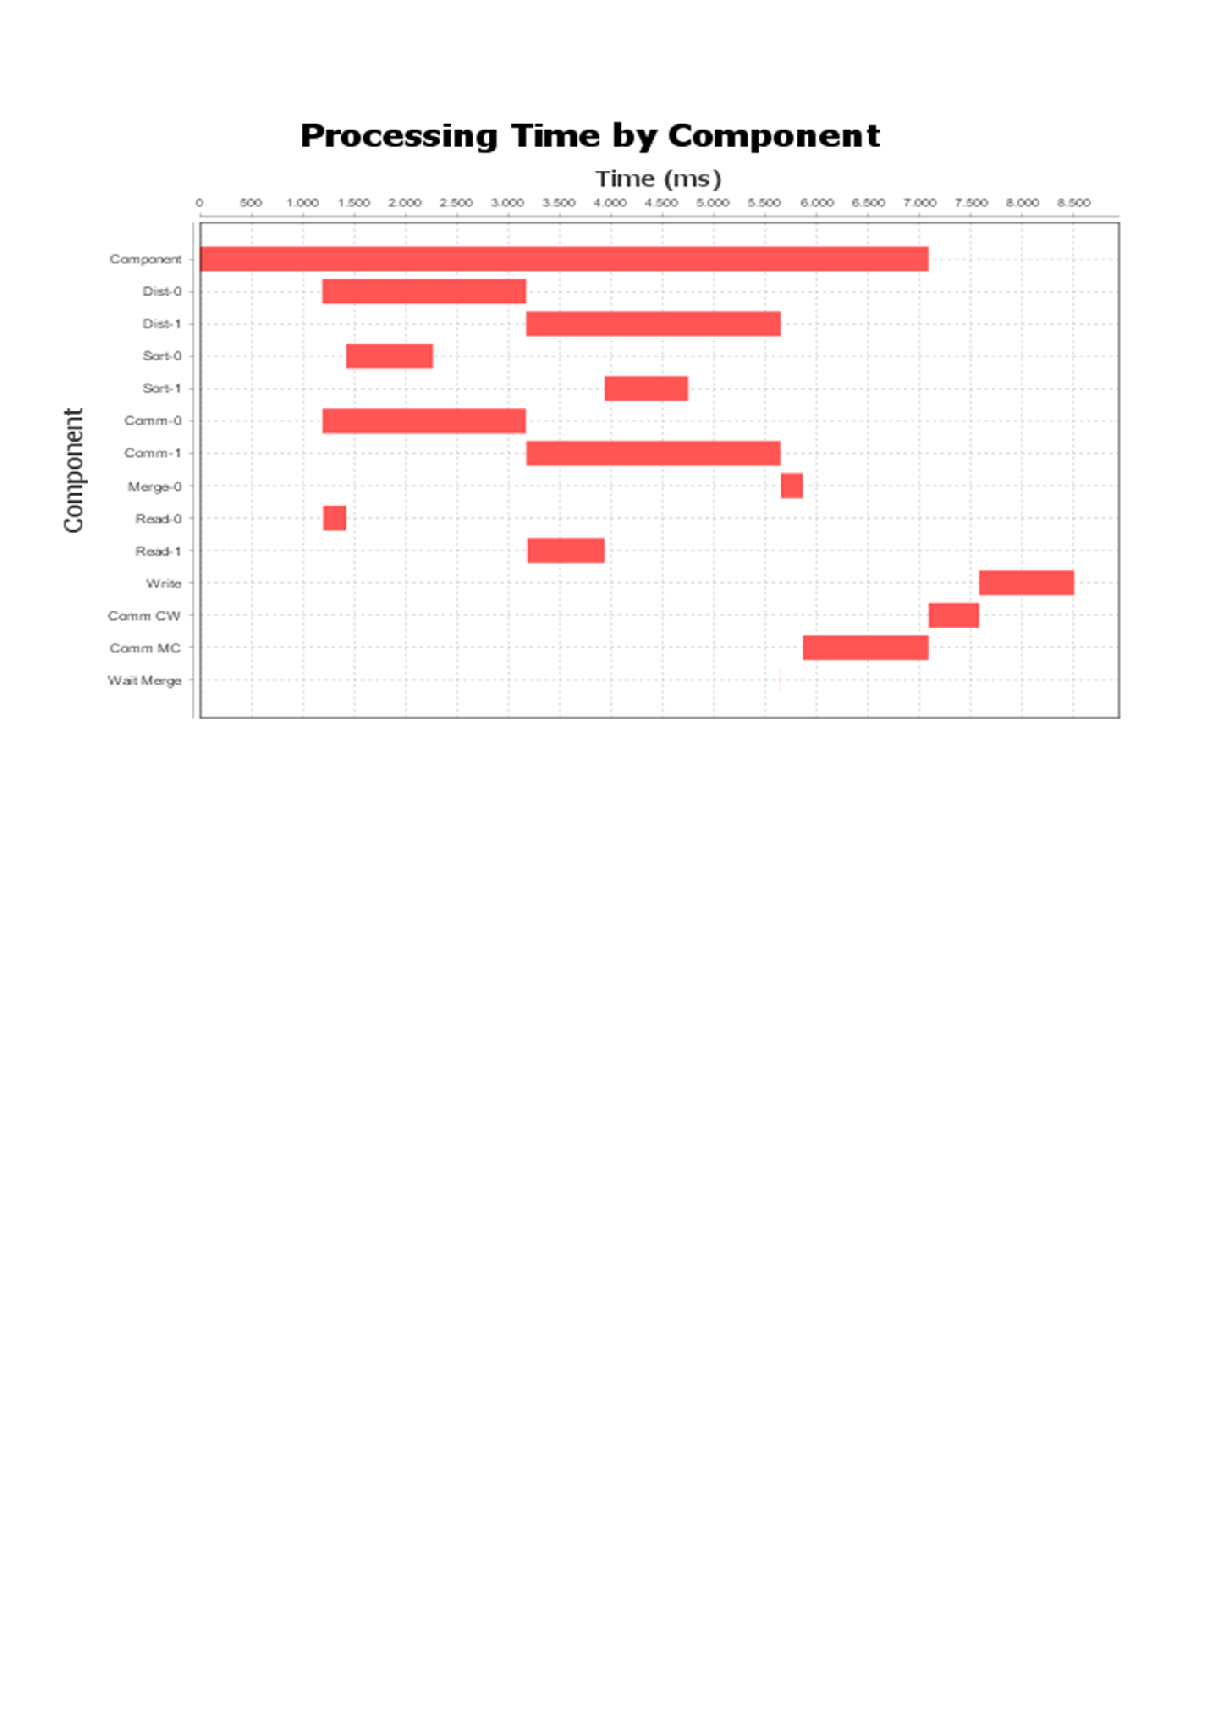
\includegraphics[trim=0.5cm 17cm -5cm 1cm, scale=0.9]{fig/LFUmaIce438Behavior.eps}
	\caption{Behavior of the Leader-Followers Design Pattern (UMA-ICE)}
	\label{fig:leaderFollowersBehaviorIce}
\end{figure}

\begin{figure}[H]
	\centering
	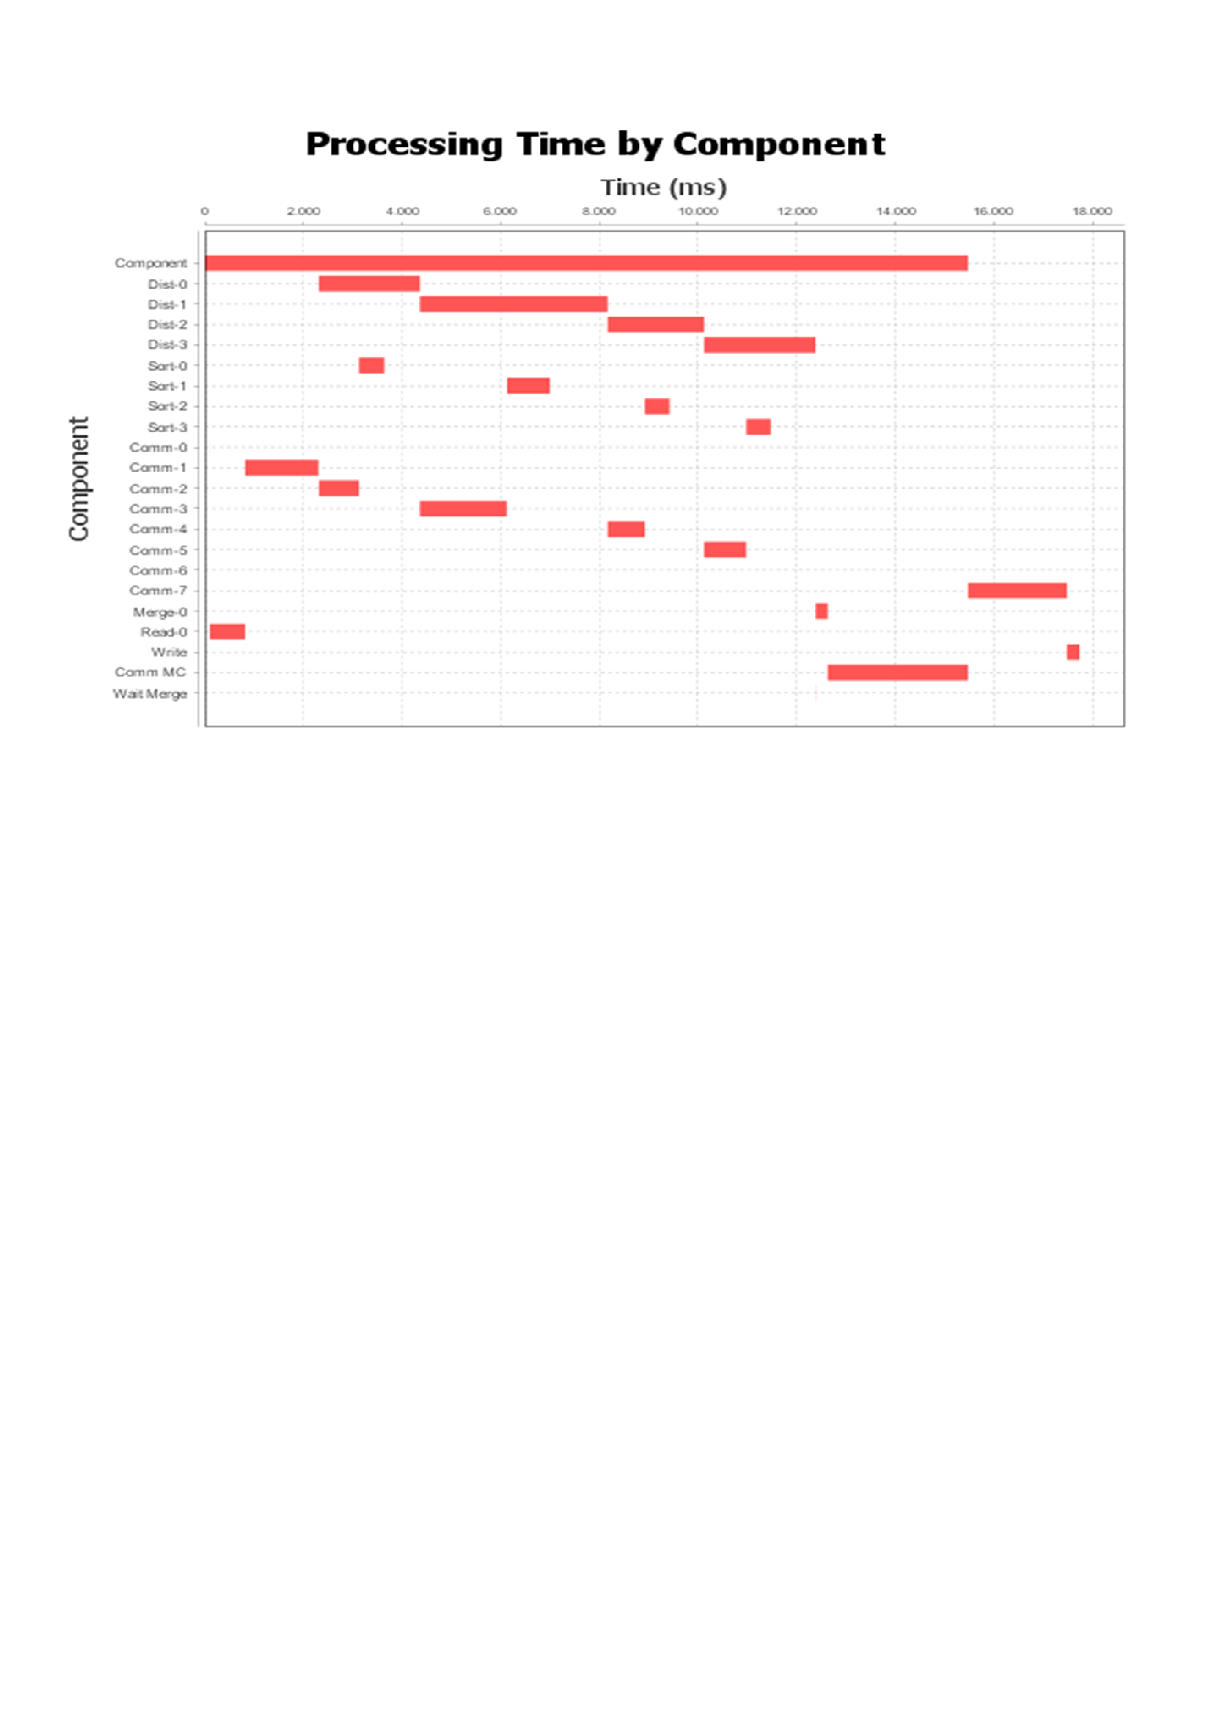
\includegraphics[trim=0.5cm 17cm -5cm 1cm, scale=0.9]{fig/LFNormaRest242Behavior.eps}
	\caption{Behavior of the Leader-Followers Design Pattern (NORMA-REST)}
	\label{fig:leaderFollowersBehaviorRest}
\end{figure}

\begin{figure}[H]
	\centering
	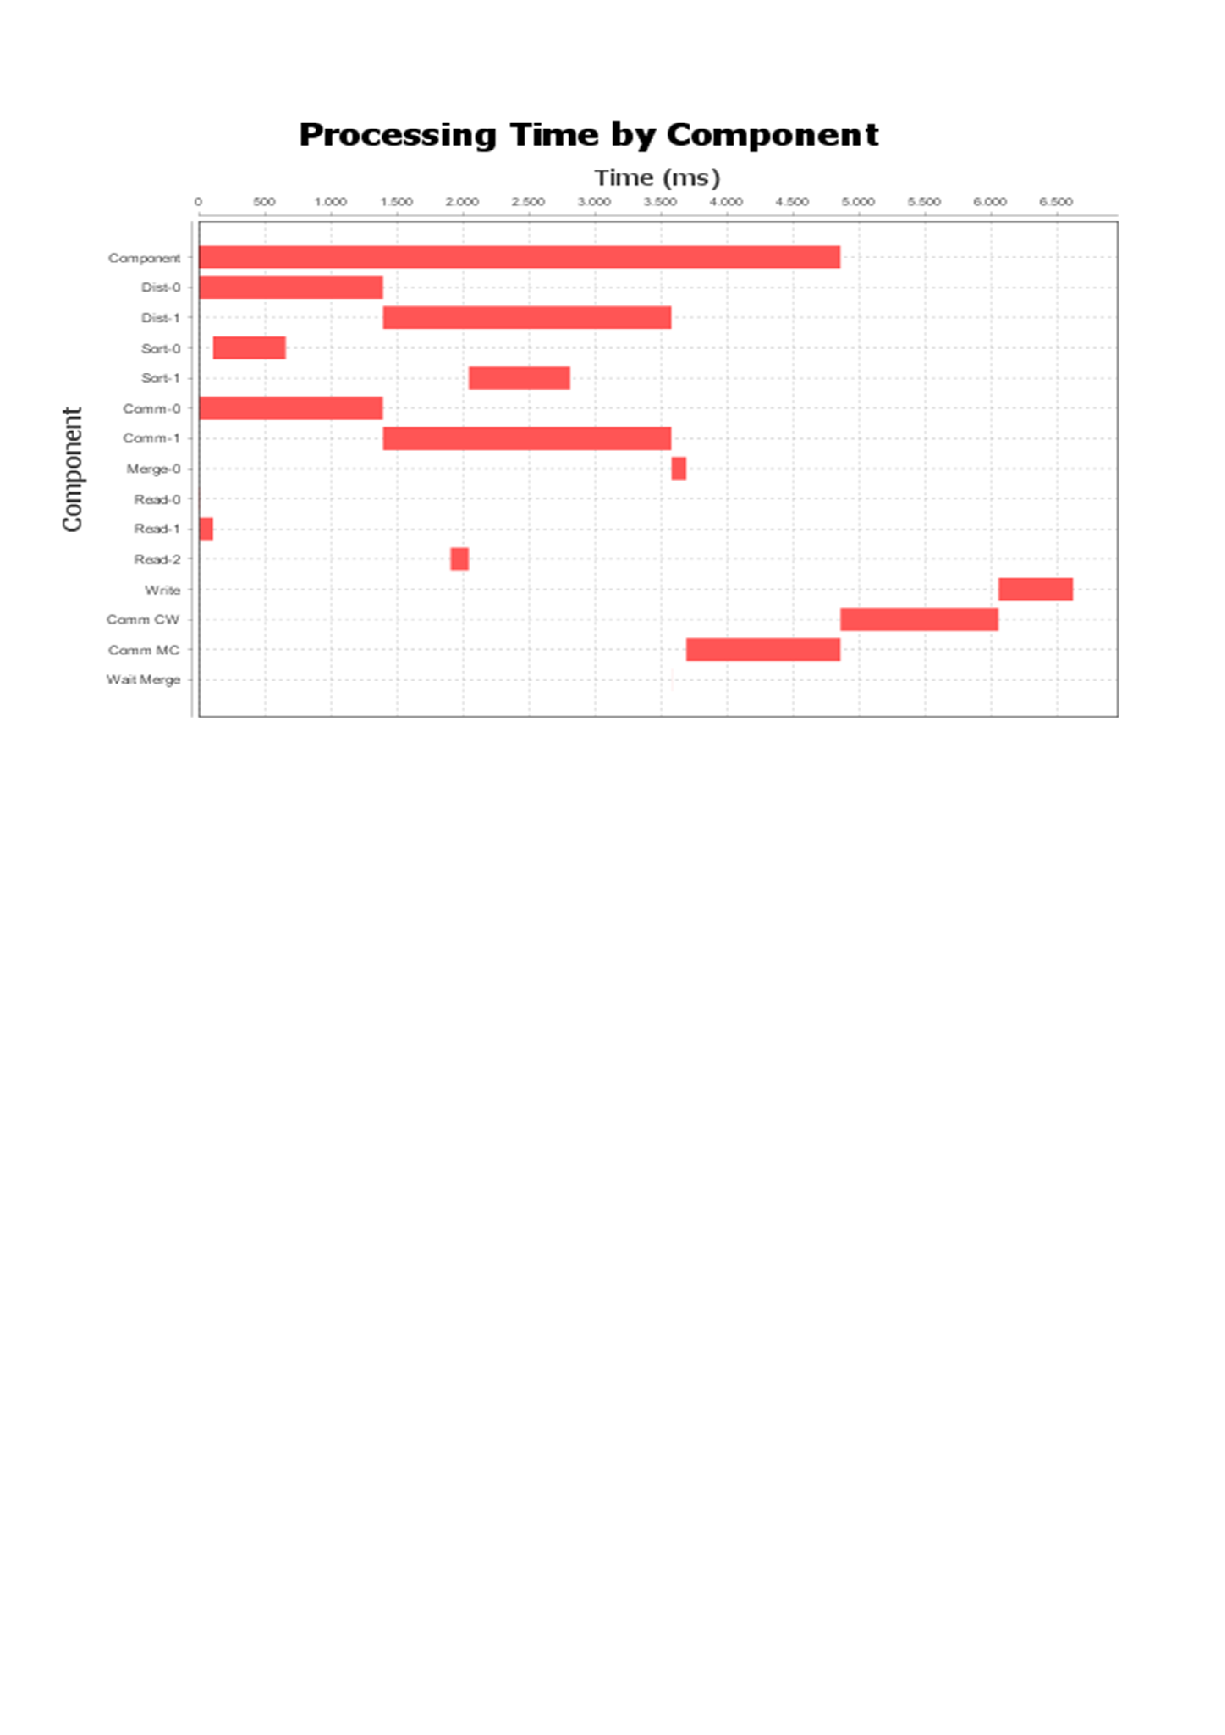
\includegraphics[trim=0.5cm 17cm -5cm 1cm, scale=0.9]{fig/LFUmaRmi422Behavior.eps}
	\caption{Behavior of the Leader-Followers Design Pattern (UMA-RMI)}
	\label{fig:leaderFollowersBehaviorRmi}
\end{figure}


\section{Latency Experiments Results}

\subsection{Consolidated Data of the Experiments Results of Controllable Variables}
\label{sebsec:consolidatedData}

Tables \ref{tab:processOriginalStrategy }, \ref{tab:processSeparationMerge}, \ref{tab:processForkJoinlibrary}, \ref{tab:processDistributedForkJoin}, and \ref{tab:processLeaderFollowers} show the experiments average processing time measured in milliseconds. For each experiments was sorted 10 files of the same size. We calculate average time for the 10 files and consolidate this information discriminating by domain-specific design pattern, communication protocol, memory structure, available nodes, and file size. Taking these tables as base we analyze each controllable variable in following sections.

According to table \ref{tab:benchmarks} we should execute 3150 experiments in the bandwidth configuration of 1GB, however, due to the thesis scope we reduce to 2561 experiments. 53,48\% of the excluded experiments correspond to the configuration of the NORMA memory structure. Due to distribution can not be leveraged in this configuration, we decide that these experiments should not be executed (see section \ref{subsec:memoryAnalysis}). 35,99\% of the excluded experiments correspond to the configuration of 16 available nodes. This decision was taken because we observe that this configuration did not improve the performance of the experiments (see section \ref{subsec:processingNodesAnalysis}).
% The 10.53\% of the excluded experiments were not executed due to previous to execute experiments of the configuration of Leader / Followers - UMA shows that this pattern had not the best results (see section \ref{}). 

The experiments of the bandwidth configuration of 100MB took too much time, therefore, taking into account the thesis scope we decide to execute just 231 experiments. These experiments were executed to verify that there is a factor of approximately 10 between the bandwidth configurations of 1GB and 100Mb. The experiments were executed in the four best configurations and four complementary configurations (see section \ref{subsec:bandwidthAnalysis}). Table \ref{tab:consolidatedData100MB} summarizes the average time of the experiments in 100MB configuration.

The missing rate of experiments was 0.078\% because only two experiments of 2561 were failed.

\begin{landscape}
	
\begin{figure}
	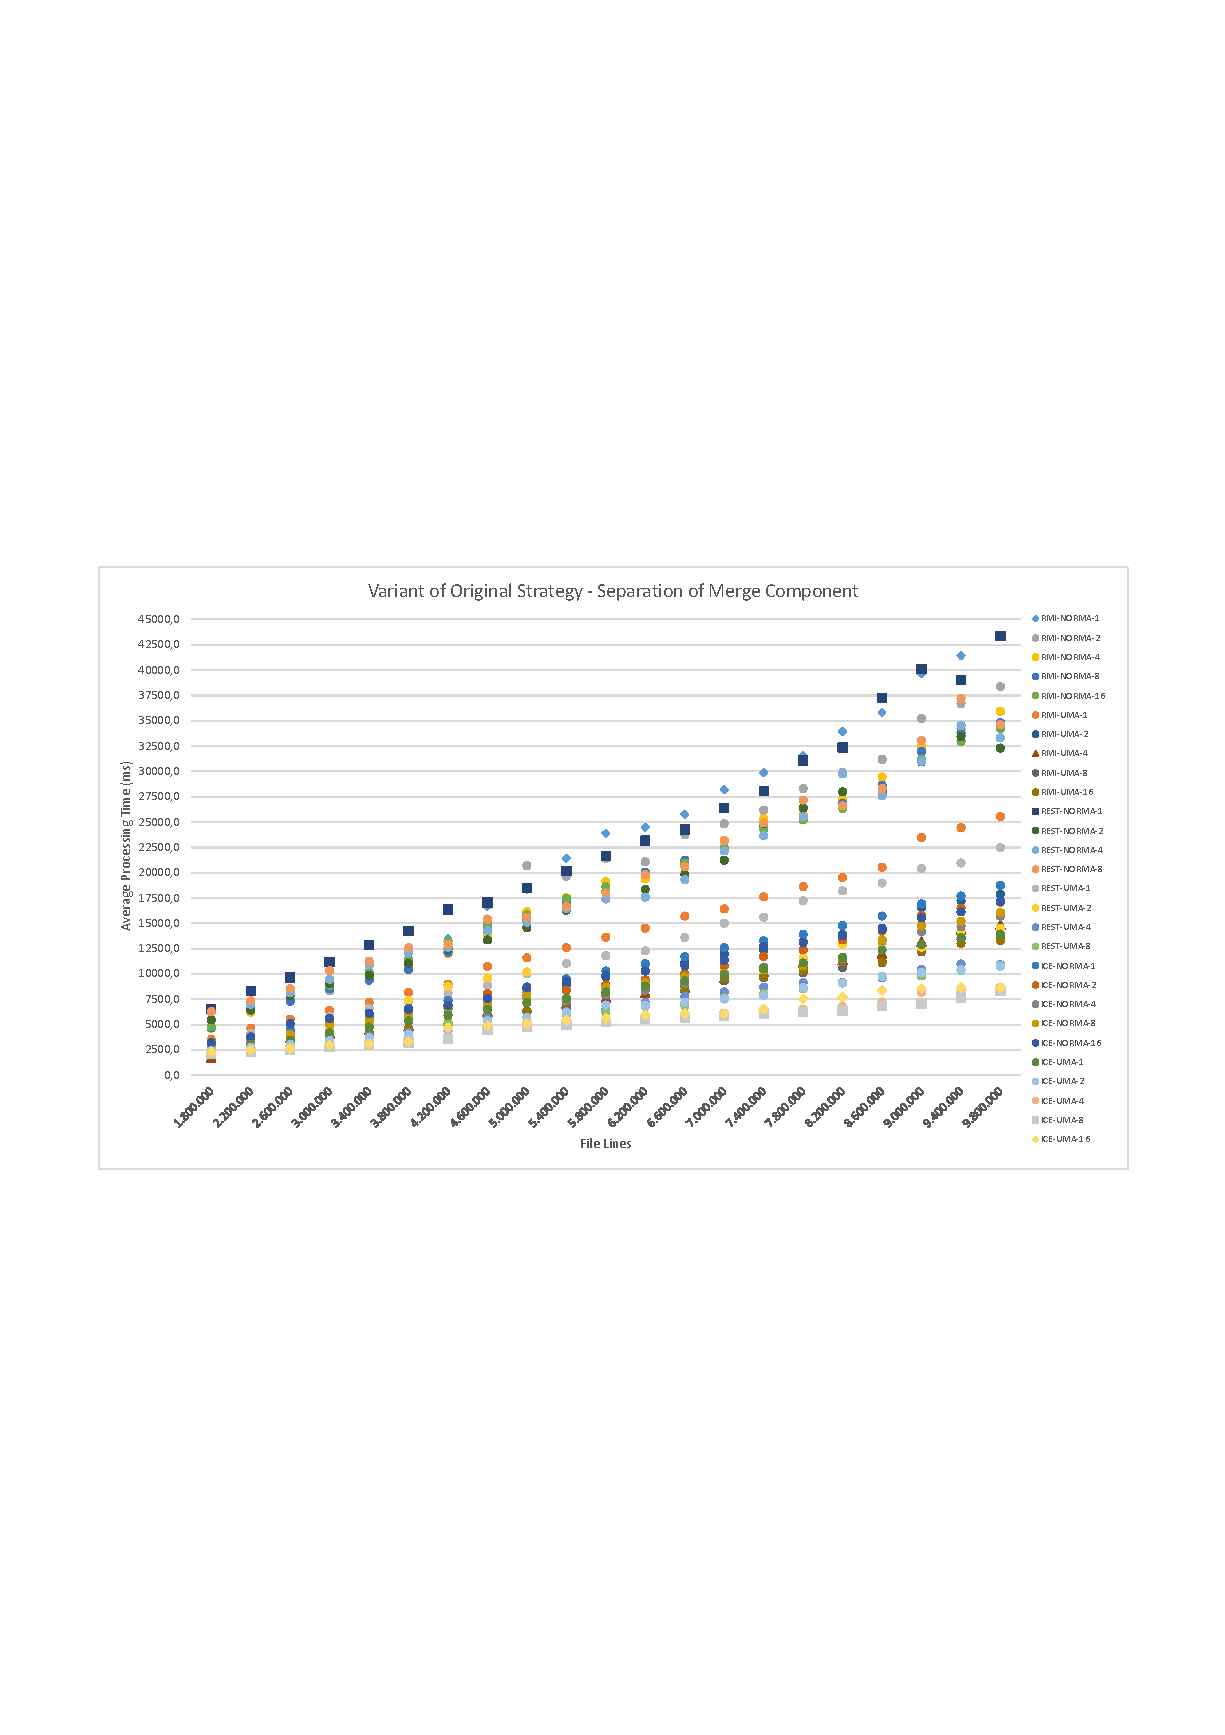
\includegraphics[trim=1cm 8cm -1cm 8cm, scale=1.3]{fig/variantOriginalStrategyGraph.eps}
	\caption{Consolidated Data of the Experiments Results of the Variant of Original Strategy - Separation of Merge Component}
	\label{fig:variantOriginalStrategyConsolidated}
\end{figure}

	% Please add the following required packages to your document preamble:
	% \usepackage{multirow}
	% \usepackage{graphicx}
	\begin{table}[]
		\centering
		\fontsize{12}{24}\selectfont
		\caption{Processing Average Time - Original Strategy - UMA}
		\label{tab:processOriginalStrategy }
		\resizebox{1.2\textwidth}{!}{%
			\begin{tabular}{|c|c|c|c|c|c|c|c|c|c|c|c|c|c|c|}
				\hline
				\multirow{3}{*}{FILE SIZE} & \multicolumn{14}{c|}{Processing Average Time - Original Strategy - UMA (ms)} \\ \cline{2-15} 
				& \multicolumn{5}{c|}{RMI} & \multicolumn{4}{c|}{REST} & \multicolumn{5}{c|}{ICE} \\ \cline{2-15} 
				& 1 & 2 & 4 & 8 & 16 & 1 & 2 & 4 & 8 & 1 & 2 & 4 & 8 & 16 \\ \hline
				1.800.000 & 2399,1 & 2390,8 & 2538,9 & 2768,1 & 2986 & 2248,2 & 2386,1 & 2424,1 & 2545 & 2228,0 & 1839,0 & 1744,5 & 1705,6 & 2162,2 \\ \hline
				2.200.000 & 3211,9 & 3111,6 & 3232,2 & 3386,1 & 3704,5 & 2889,8 & 2812,9 & 2932,2 & 3386,7 & 2597,2 & 2367,3 & 2280,5 & 2029,9 & 2576,6 \\ \hline
				2.600.000 & 3734,2 & 3633,4 & 3734,3 & 3945,7 & 4301,8 & 3330,5 & 3286 & 3328 & 3722 & 3122,0 & 2588,4 & 2639,5 & 2367,3 & 2294,5 \\ \hline
				3.000.000 & 4319,5 & 4196,8 & 4200,6 & 4449,6 & 4797,2 & 4016,6 & 3679,8 & 3833 & 4236,9 & 3662,5 & 3454,2 & 3287,1 & 3313,7 & 3433,6 \\ \hline
				3.400.000 & 4916,2 & 4693,1 & 4763,5 & 5087,5 & 5434,9 & 4607,6 & 4216,1 & 4354,4 & 4794,4 & 4179,8 & 3952,1 & 3687,2 & 3714,4 & 3785,0 \\ \hline
				3.800.000 & 5596,3 & 5235,4 & 5312,4 & 5530 & 5870,7 & 8037,1 & 6746,5 & 5060,5 & 5292 & 4677,4 & 4346,8 & 4128,1 & 4105,3 & 4163,6 \\ \hline
				4.200.000 & 5990,2 & 5827 & 5831,7 & 6190,2 & 6449,4 & 6934 & 5567,6 & 5429,2 & 5901,3 & 5217,5 & 4830,3 & 4505,2 & 4416,1 & 4639,2 \\ \hline
				4.600.000 & 7686,9 & 6770,5 & 6665,3 & 7037,9 & 7343,5 & 6113,3 & 6223,8 & 5916,1 & 6448,7 & 5730,9 & 5274,6 & 4934,1 & 4849,1 & 4938,3 \\ \hline
				5.000.000 & 8004,9 & 7281,8 & 7271 & 7669,6 & 7944,3 & 6710,9 & 6402,6 & 6434,1 & 6421,7 & 6280,7 & 5720,2 & 5304,1 & 5263,3 & 5375,5 \\ \hline
				5.400.000 & 8890,1 & 7940,3 & 7958,3 & 8309,3 & 8591,8 & 7755,8 & 7308,3 & 7191,2 & 7232,3 & 6977,3 & 6162,0 & 5697,4 & 5440,5 & 5685,6 \\ \hline
				5.800.000 & 9758,1 & 8878,3 & 8649,4 & 9172 & 9427,1 & 8622,7 & 7726,6 & 7898,2 & 6965 & 7607,6 & 6837,6 & 6206,0 & 5934,8 & 6045,2 \\ \hline
				6.200.000 & 10268 & 9415,2 & 9296,4 & 9693,5 & 10137,2 & 9661,9 & 8435,6 & 8163,1 & 8347,4 & 8179,1 & 7093,8 & 6592,0 & 6245,3 & 6197,7 \\ \hline
				6.600.000 & 11087,2 & 9987,6 & 9875 & 10266,2 & 10600,6 & 10423,4 & 9064,1 & 8878,7 & 8973,9 & 8778,6 & 7621,0 & 6886,9 & 6686,5 & 7058,9 \\ \hline
				7.000.000 & 12023,1 & 10351,9 & 10672,8 & 11019,1 & 11159,8 & 10806,4 & 9548,9 & 9226,7 & 9992,1 & 9278,3 & 8033,1 & 7415,3 & 6974,6 & 7384,9 \\ \hline
				7.400.000 & 12851,7 & 11072,8 & 11208,2 & 11503,3 & 11995,1 & 12404,6 & 11205,8 & 9267,1 & 10295,5 & 9788,1 & 8510,6 & 7754,8 & 7372,7 & 7691,9 \\ \hline
				7.800.000 & 13777,6 & 11883,2 & 11759,4 & 12225,1 & 12847,1 & 13227,4 & 11122,6 & 9552,3 & 10507,4 & 10482,5 & 9108,1 & 8194,8 & 7726,1 & 7999,4 \\ \hline
				8.200.000 & 14152,8 & 12486,2 & 12639,4 & 12559,6 & 13493,9 & 13505,8 & 12040,7 & 11528,6 & 11403,7 & 11027,1 & 9630,6 & 8512,3 & 8077,6 & 8277,1 \\ \hline
				8.600.000 & 15558 & 13274,7 & 13409,7 & 13412,5 & 14216,8 & 14527,7 & 12680,1 & 11406,7 & 11988,1 & 11795,7 & 10167,4 & 8961,1 & 8552,8 & 8662,9 \\ \hline
				9.000.000 & 16738,7 & 14754,8 & 14989 & 15359,8 & 15590,4 & 16384,7 & 14221,2 & 11399,5 & 12061,6 & 12333,4 & 10189,8 & 9305,3 & 8864,7 & 9333,5 \\ \hline
				9.400.000 & 18149,5 & 15234,6 & 15426,6 & 16167 & 16354,9 & 14441,5 & 13152,3 & 12949,6 & 12540,4 & 13182,2 & 10773,4 & 9676,8 & 9240,9 & 9595,3 \\ \hline
				9.800.000 & 19389,9 & 16185,8 & 16540,6 & 16798,6 & 17022,9 & 16812,6 & 14586,2 & 13704,6 & 14133,9 & 13692,9 & 11219,4 & 10069,0 & 9521,5 & 9998,2 \\ \hline
			\end{tabular}%
		}
	\end{table}
	
% Please add the following required packages to your document preamble:
% \usepackage{multirow}
% \usepackage{graphicx}
\begin{table}[]
	\fontsize{12}{24}\selectfont
	\centering
	\caption{Processing Average Time - Variant of Original Strategy - Separation of Merge Component}
	\label{tab:processSeparationMerge}
	\resizebox{1.45\textwidth}{!}{%
		\begin{tabular}{|c|c|c|c|c|c|c|c|c|c|c|c|c|c|c|c|c|c|c|c|c|c|c|c|c|c|c|c|c|}
			\hline
			\multirow{4}{*}{FILE SIZE} & \multicolumn{28}{c|}{Processing Average Time - Variant of Original Strategy - Separation of Merge Component  (ms)} \\ \cline{2-29} 
			& \multicolumn{10}{c|}{RMI} & \multicolumn{8}{c|}{REST} & \multicolumn{10}{c|}{ICE} \\ \cline{2-29} 
			& \multicolumn{5}{c|}{NORMA} & \multicolumn{5}{c|}{UMA} & \multicolumn{4}{c|}{NORMA} & \multicolumn{4}{c|}{UMA} & \multicolumn{5}{c|}{NORMA} & \multicolumn{5}{c|}{UMA} \\ \cline{2-29} 
			& 1 & 2 & 4 & 8 & 16 & 1 & 2 & 4 & 8 & 16 & 1 & 2 & 4 & 8 & 1 & 2 & 4 & 8 & 1 & 2 & 4 & 8 & 16 & 1 & 2 & 4 & 8 & 16 \\ \hline
			1.800.000 & 5594,7 & 4829,5 & 4653,9 & 4676,8 & 4797,7 & 3555,5 & 2809,1 & 1781,7 & 2765,9 & 2750,3 & 6573,7 & 5491,3 & 6273,3 & 6308 & 3210,7 & 2123,9 & 2776,5 & 2529,8 & 2895,9 & 3198,9 & 2905,6 & 2849,3 & 3219,6 & 2420,9 & 2464,2 & 2163,9 & 2104,1 & 2327,8 \\ \hline
			2.200.000 & 6671,9 & 6384,6 & 6225,5 & 6448,7 & 7156,2 & 4670,6 & 3398,9 & 2327 & 3174,6 & 3164,1 & 8341,1 & 6493,8 & 7026,5 & 7399,6 & 4153,9 & 3540,9 & 2946,9 & 2817,5 & 3836,9 & 3614,5 & 3304,4 & 3205,4 & 3792,9 & 3077,1 & 2770,6 & 2374,6 & 2302,6 & 2508,9 \\ \hline
			2.600.000 & 8000,7 & 7490,2 & 7368,9 & 7316,8 & 8235,1 & 5552,3 & 4507,2 & 3667,4 & 3487,8 & 3507,7 & 9648,7 & 7866,0 & 8146,2 & 8555,1 & 4985,1 & 3942,4 & 3258,9 & 3081,3 & 4524,8 & 4057,6 & 3662,5 & 4069,5 & 5128,8 & 3475,2 & 3058,1 & 2603,1 & 2521,0 & 2662,7 \\ \hline
			3.000.000 & 9180,4 & 8358,4 & 8811,1 & 8564,6 & 8902,2 & 6414,9 & 4976 & 4133,1 & 3866,6 & 3823 & 11197,3 & 9055,1 & 9484,6 & 10352,1 & 5798,1 & 4496 & 3589,4 & 3311,8 & 5324,9 & 5055,2 & 4114,5 & 5009,9 & 5638,8 & 4229,5 & 3442,3 & 2873,1 & 2777,3 & 3038,1 \\ \hline
			3.400.000 & 10349,4 & 9456,7 & 9753,1 & 9395,5 & 10148,4 & 7202 & 5485,1 & 4444,3 & 4170 & 4235 & 12858 & 9889,8 & 10928,4 & 11265,9 & 6601 & 5108,2 & 3889,8 & 3736,3 & 5982,1 & 5557,5 & 5493,7 & 5400,9 & 6134,3 & 4790,1 & 3740,0 & 3072,9 & 2976,5 & 3137,2 \\ \hline
			3.800.000 & 11586,9 & 10623,6 & 10752,6 & 10472,6 & 11346,1 & 8203,3 & 6054,6 & 4854,1 & 4564,7 & 4615,1 & 14264,3 & 11083,3 & 12132,4 & 12611,8 & 13743,7 & 7374 & 4236,2 & 5788,6 & 6642,1 & 6068,9 & 6297,6 & 6024,6 & 6487,7 & 5376,4 & 4075,9 & 3330,5 & 3256,9 & 3348,1 \\ \hline
			4.200.000 & 13480,2 & 12195,0 & 12019,1 & 12154,8 & 13226,6 & 8990,2 & 6597,5 & 5262,4 & 4923,1 & 5155,1 & 16384,2 & 12464,7 & 12640,2 & 12933,9 & 16027,1 & 8767,3 & 4648,6 & 5049,9 & 7385,5 & 6978,3 & 6838,5 & 6677,4 & 6912,1 & 5930,8 & 4399,3 & 3639,1 & 3577,2 & 4692,9 \\ \hline
			4.600.000 & 16690,0 & 15367,5 & 13878,6 & 14492,7 & 14941,0 & 10784 & 7761,3 & 6246,2 & 5689,8 & 5893,2 & 17077,1 & 13378,7 & 14305,6 & 15438,3 & 23997,8 & 9614,4 & 5656,5 & 7322,6 & 8037,2 & 8060,9 & 7582,4 & 7043,5 & 7594,1 & 6543,6 & 5373,7 & 4563,1 & 4502,9 & 4937,7 \\ \hline
			5.000.000 & 18352,9 & 20706,5 & 16159,4 & 15421,8 & 15852,1 & 11634,8 & 8318,3 & 6624,2 & 6271,8 & 6388,8 & 18504 & 14601,0 & 15132 & 15598,7 & 10033,9 & 10214 & 7923,5 & 8423,1 & 8718,5 & 8574,3 & 7672,0 & 7842,1 & 8682,7 & 7202,3 & 5718,5 & 4990,8 & 4821,3 & 5114,5 \\ \hline
			5.400.000 & 21453,5 & 19675,2 & 17559,0 & 16981,4 & 17463,8 & 12622,8 & 9010,1 & 7074,1 & 6956,4 & 7238,4 & 20191,9 & 16318,2 & 16462,4 & 16692,7 & 11059,8 & 7420,3 & 6342,5 & 6022,3 & 9524,7 & 8419,7 & 7433,4 & 7601,6 & 9253,5 & 7604,7 & 6209,9 & 5185,7 & 4998,3 & 5487,3 \\ \hline
			5.800.000 & 23901,7 & 21431,8 & 19121,0 & 18206,0 & 18623,0 & 13640,7 & 9762,7 & 7679,4 & 7946,9 & 8147,3 & 21631,8 & 17411,2 & 17416,3 & 18031,2 & 11820,1 & 8404,1 & 6477,4 & 6243,9 & 10310,0 & 8935,9 & 7971,9 & 8700,2 & 9872,2 & 8237,8 & 6944,2 & 5459,9 & 5255,7 & 5630,3 \\ \hline
			6.200.000 & 24526,2 & 21093,0 & 19404,9 & 20067,3 & 19860,4 & 14526,7 & 10356,3 & 8161,3 & 8433,1 & 8455,3 & 23165,8 & 18359,4 & 17596,4 & 19790,7 & 12291,7 & 8700,7 & 7202,4 & 6817,6 & 11022,2 & 9440,8 & 8407,6 & 9164,3 & 10303,2 & 8797,2 & 6933,2 & 5714,4 & 5608,3 & 5956,5 \\ \hline
			6.600.000 & 25791,9 & 23765,5 & 21214,1 & 21247,3 & 20939,6 & 15727,3 & 11131,1 & 8661,7 & 8821,7 & 8438,1 & 24251,2 & 19833,3 & 19338,3 & 20583 & 13618,4 & 9339,5 & 7803 & 6875,5 & 11722,6 & 10025,8 & 9107,9 & 9729,0 & 10847,1 & 9370,3 & 7222,6 & 5895,7 & 5660,8 & 6113,1 \\ \hline
			7.000.000 & 28216,4 & 24848,3 & 23227,5 & 22422,7 & 22426,9 & 16432,1 & 11971,3 & 9613,4 & 9355,8 & 9542,2 & 26389,1 & 21240,7 & 22156,7 & 23142,1 & 15018,6 & 9970,6 & 8232,3 & 7656,2 & 12606,7 & 10807,1 & 10081,5 & 10056,0 & 11378,0 & 9914,5 & 7535,1 & 6138,9 & 5855,3 & 6102,5 \\ \hline
			7.400.000 & 29904,6 & 26163,7 & 25325,9 & 24478,9 & 24289,1 & 17630,9 & 12350,8 & 10199,7 & 9643,4 & 9783,5 & 28092,2 & 24881,2 & 23676,4 & 24910 & 15618,9 & 10422,4 & 8705,4 & 8061,3 & 13294,4 & 11739,5 & 10689,3 & 10446,0 & 12750,5 & 10526,1 & 7865,8 & 6360,5 & 6071,7 & 6553,4 \\ \hline
			7.800.000 & 31582,4 & 28327,0 & 25702,6 & 25478,3 & 25232,1 & 18648,5 & 13163 & 11095,9 & 10157 & 10378,3 & 31098,9 & 26382,6 & 25523,5 & 27172,6 & 17260,4 & 11581,9 & 9166,2 & 8539,2 & 13917,8 & 12389,8 & 11107,8 & 10839,7 & 13116,9 & 11102,0 & 8648,3 & 6540,1 & 6275,5 & 7551,6 \\ \hline
			8.200.000 & 33962,8 & 29881,0 & 27190,7 & 26879,0 & 26371,8 & 19528,8 & 13902,7 & 11380 & 10626,8 & 11229,1 & 32374,6 & 27984,6 & 29757,4 & 26618,2 & 18207,1 & 12929,1 & 9188,2 & 9140,2 & 14786,4 & 13370,9 & 11532,4 & 11625,0 & 13787,3 & 11677,4 & 9118,9 & 6795,0 & 6402,3 & 7784,0 \\ \hline
			8.600.000 & 35820,9 & 31194,8 & 29462,1 & 28634,8 & 27821,8 & 20541 & 14511,4 & 11996,4 & 11123,5 & 11228,9 & 37241,5 & 28013,8 & 27629,2 & 28323,1 & 18990,1 & 12952,5 & 9613,7 & 9803,6 & 15734,5 & 14292,6 & 13304,6 & 13402,0 & 14416,8 & 12379,4 & 9791,0 & 7261,0 & 6839,2 & 8397,3 \\ \hline
			9.000.000 & 39668,1 & 35228,1 & 32479,0 & 31984,2 & 31222,6 & 23471,8 & 16579,7 & 13210 & 12192,4 & 12378,2 & 40087,8 & 30950,8 & 31038,2 & 33042,2 & 20416,6 & 12680 & 10450,4 & 9813,9 & 16933,7 & 15761,0 & 14219,5 & 14793,9 & 15548,7 & 12921,6 & 10150,9 & 8215,3 & 7117,3 & 8592,5 \\ \hline
			9.400.000 & 41421,8 & 36717,8 & 34212,1 & 33836,6 & 32973,5 & 24460,7 & 17252,2 & 14375,9 & 13448,4 & 13047,2 & 38996,2 & 33457,1 & 34531,1 & 37203,4 & 20957 & 14308,4 & 10995,1 & 10375,1 & 17701,2 & 16515,9 & 14695,9 & 15212,5 & 16152,3 & 13620,1 & 10448,9 & 8425,5 & 7691,2 & 8666,5 \\ \hline
			9.800.000 & 43339,0 & 38376,8 & 35943,9 & 34841,4 & 34235,8 & 25544,6 & 17897,5 & 14877,2 & 13562,2 & 13318 & 43393,4 & 32308,9 & 33330 & 34639,8 & 22495,2 & 14533,4 & 10948,9 & 10860,6 & 18769,5 & 17102,6 & 15725,7 & 16081,3 & 17162,6 & 13953,4 & 10785,7 & 8712,0 & 8299,0 & 8626,6 \\ \hline
		\end{tabular}%
	}
\end{table}

% Please add the following required packages to your document preamble:
% \usepackage{multirow}
% \usepackage{graphicx}
\begin{table}[]
	\fontsize{12}{24}\selectfont
	\centering
	\caption{Processing Average Time - Fork/Join Java library}
	\label{tab:processForkJoinlibrary}
	\resizebox{1.45\textwidth}{!}{%
		\begin{tabular}{|c|c|c|c|c|c|c|c|c|c|c|c|c|c|c|c|c|c|c|c|c|c|c|c|c|c|c|c|c|}
			\hline
			\multirow{4}{*}{FILE SIZE} & \multicolumn{28}{c|}{Processing Average Time - Fork/Join Java library (ms)} \\ \cline{2-29} 
			& \multicolumn{10}{c|}{RMI} & \multicolumn{8}{c|}{REST} & \multicolumn{10}{c|}{ICE} \\ \cline{2-29} 
			& \multicolumn{5}{c|}{NORMA} & \multicolumn{5}{c|}{UMA} & \multicolumn{4}{c|}{NORMA} & \multicolumn{4}{c|}{UMA} & \multicolumn{5}{c|}{NORMA} & \multicolumn{5}{c|}{UMA} \\ \cline{2-29} 
			& 1 & 2 & 4 & 8 & 16 & 1 & 2 & 4 & 8 & 16 & 1 & 2 & 4 & 8 & 1 & 2 & 4 & 8 & 1 & 2 & 4 & 8 & 16 & 1 & 2 & 4 & 8 & 16 \\ \hline
			1.800.000 & 6049,9 & 5102,4 & 4630,5 & 5478,6 & 5127,2 & 3468,1 & 3519,9 & 2550,20 & 2979,80 & 3283,7 & 5992 & 5453,0 & 5715,6 & 5798,6 & 3474,9 & 2813 & 3129,8 & 3021,1 & 3021,5 & 3409,5 & 3631,5 & 3545,8 & 3932,6 & 2132,3 & 2638,6 & 2443,4 & 2362,1 & 2518,7 \\ \hline
			2.200.000 & 6651,7 & 6127,1 & 5676,4 & 6290,0 & 6691,3 & 4454,4 & 4138,5 & 2994,90 & 3260,70 & 3711,7 & 7450,4 & 6048,2 & 6804,3 & 7208,9 & 4142,6 & 3864,8 & 3417,9 & 3287,9 & 3941,5 & 4127,8 & 3938,4 & 4400,3 & 4322,5 & 2753,6 & 2908,8 & 2627,6 & 2539,1 & 2695,1 \\ \hline
			2.600.000 & 9218,5 & 7382,0 & 7125,9 & 7117,9 & 8534,5 & 4990,7 & 4555,1 & 3694,10 & 3660,20 & 4009,2 & 8846,5 & 7178,7 & 7328 & 9483,4 & 4748,3 & 4391,9 & 3656,6 & 3531 & 4482,0 & 5003,5 & 4607,7 & 5179,6 & 4854,0 & 3104,7 & 3095,6 & 2806,6 & 2703,6 & 2860,3 \\ \hline
			3.000.000 & 9933,1 & 8066,5 & 8004,4 & 8924,6 & 9422,8 & 5673,6 & 4965 & 4159,90 & 3862,50 & 4404,7 & 9453,5 & 8269 & 8434,7 & 10064,3 & 5383 & 4684,1 & 4001,7 & 3817,1 & 5159,3 & 5042,7 & 4945,7 & 5241,4 & 5236,5 & 3374,1 & 3416,3 & 3003,4 & 2886,1 & 3059,1 \\ \hline
			3.400.000 & 11580,9 & 8913,3 & 8484,5 & 8954,7 & 10795,7 & 6425,5 & 5368,8 & 4390,40 & 4163,10 & 4774,1 & 11355,7 & 9092,3 & 9626,2 & 11527,1 & 8784,8 & 5151 & 4281,6 & 4095,7 & 5726,6 & 5432,7 & 6154,9 & 5242,8 & 6393,1 & 3988,7 & 3795,0 & 3262,9 & 3054,4 & 3488,1 \\ \hline
			3.800.000 & 12416,4 & 10955,2 & 11193,5 & 11639,2 & 12153,0 & 7051,8 & 5753,1 & 4904,70 & 4291,80 & 5146,9 & 12508,6 & 10067,1 & 10399,1 & 11877,2 & 15118 & 5658,5 & 4553 & 4606,1 & 6313,7 & 5882,1 & 6288,7 & 6064,3 & 7275,1 & 4149,0 & 4016,4 & 3481,6 & 3307,0 & 3294,2 \\ \hline
			4.200.000 & 13798,9 & 12161,1 & 12368,0 & 13089,4 & 13409,1 & 7612,3 & 5853,6 & 5038,00 & 4694,20 & 5623,6 & 13335,7 & 10980,1 & 13102,4 & 13172 & 7537,1 & 6049 & 5049 & 5174,3 & 6903,2 & 6483,3 & 6718,5 & 6746,7 & 7485,8 & 4627,0 & 4240,3 & 3657,0 & 4086,0 & 4522,3 \\ \hline
			4.600.000 & 16010,8 & 14411,3 & 14118,0 & 15397,9 & 15650,3 & 9168,8 & 6338,3 & 6021,80 & 5620,50 & 6520,8 & 14744,1 & 11618,5 & 13654,2 & 14678,6 & 8900,5 & 6747,2 & 5251,6 & 5718,9 & 7468,6 & 6795,8 & 7183,4 & 7886,6 & 7911,1 & 5797,2 & 4503,6 & 3869,0 & 4751,6 & 4671,9 \\ \hline
			5.000.000 & 17515,8 & 15807,5 & 15141,1 & 16405,6 & 16975,8 & 9775,5 & 6518,8 & 6117,60 & 6200,10 & 7609,3 & 16610,8 & 13064,8 & 14642,5 & 15828,2 & 20934,2 & 7538,4 & 5801,9 & 6165,2 & 8035,5 & 7309,2 & 7634,0 & 8434,1 & 8939,0 & 5402,0 & 4764,2 & 4044,7 & 4502,3 & 4769,5 \\ \hline
			5.400.000 & 19352,4 & 16923,3 & 16510,9 & 17262,0 & 18237,9 & 10499,5 & 7013,7 & 6335,20 & 6259,90 & 8016,8 & 17318,3 & 13953,7 & 17303,3 & 16357,3 & 9562,7 & 7104,2 & 6680,1 & 6466,3 & 8385,9 & 7517,6 & 7193,9 & 8467,3 & 9814,5 & 5667,5 & 5524,1 & 5039,3 & 4824,5 & 5038,7 \\ \hline
			5.800.000 & 20523,4 & 18406,1 & 18662,9 & 19049,1 & 19655,9 & 11485,4 & 7295,2 & 6613,40 & 7360,00 & 8853,5 & 18872,6 & 14911,7 & 18321,9 & 17350 & 10582,5 & 7931 & 7064,8 & 6746,6 & 9069,8 & 8206,3 & 7782,8 & 9450,5 & 10378,9 & 6090,5 & 5882,0 & 5283,7 & 5049,0 & 5275,3 \\ \hline
			6.200.000 & 23189,3 & 19855,9 & 19946,2 & 20779,4 & 20829,8 & 12052 & 7495,9 & 6412,60 & 7677,60 & 9354,2 & 19566 & 16860,6 & 18931,2 & 19199,2 & 10916,2 & 8193,5 & 7255 & 6913,5 & 9613,9 & 8555,4 & 8202,9 & 9862,6 & 10858,8 & 6513,9 & 6090,0 & 5459,8 & 5222,5 & 5607,5 \\ \hline
			6.600.000 & 25534,8 & 21719,2 & 21294,1 & 22079,8 & 22415,7 & 12977,5 & 8002,7 & 5635,30 & 7605,00 & 9668,5 & 23283,8 & 17217,6 & 20069,3 & 22010,4 & 11904,2 & 8907,7 & 7579,1 & 7602,3 & 10191,2 & 9045,4 & 8666,7 & 10220,2 & 11267,2 & 6811,3 & 6325,3 & 5576,4 & 5365,8 & 5728,7 \\ \hline
			7.000.000 & 27332,0 & 23607,2 & 22652,1 & 22989,0 & 23827,0 & 13519,5 & 10028,3 & 8174,30 & 8377,60 & 10262,1 & 24642,3 & 21848,7 & 23474,1 & 22339,5 & 12699,2 & 9709,7 & 8450,5 & 7832 & 10763,3 & 9424,9 & 9015,3 & 10595,2 & 11706,6 & 7129,7 & 6545,7 & 5824,8 & 5593,5 & 5737,1 \\ \hline
			7.400.000 & 29758,4 & 25350,9 & 24078,9 & 25421,3 & 25097,8 & 14376,1 & 10373 & 8315,70 & 8265,60 & 10631,9 & 25319,6 & 22263,2 & 25330,8 & 24969,8 & 13486,5 & 9796,9 & 8609,7 & 9028,4 & 11352,7 & 10034,7 & 9388,8 & 10916,9 & 12316,8 & 7688,0 & 6743,6 & 5963,6 & 5674,4 & 6270,0 \\ \hline
			7.800.000 & 31223,1 & 26415,6 & 25164,2 & 26628,6 & 26455,1 & 15880,7 & 10865,6 & 8486,80 & 8796,40 & 11443,4 & 29697 & 22370,3 & 27062,8 & 25731,4 & 14506,6 & 10751,4 & 9655,1 & 8598,2 & 11915,5 & 10961,5 & 9755,0 & 11444,1 & 13707,3 & 7831,7 & 7042,0 & 6116,1 & 5807,1 & 7083,0 \\ \hline
			8.200.000 & 32777,9 & 27983,1 & 26813,5 & 28168,9 & 27670,1 & 17232,4 & 11205,4 & 9127,30 & 8856,20 & 12368,2 & 29275,8 & 27287,9 & 29121,1 & 27956,5 & 14672,6 & 11050,1 & 9812,7 & 9564,2 & 12463,5 & 11548,6 & 10210,3 & 11950,8 & 14079,2 &  & 8039,3 & 6345,8 & 6118,1 & 7286,4 \\ \hline
			8.600.000 & 34163,9 & 29709,9 & 29137,9 & 29970,5 & 29173,2 & 16964,4 & 11851,4 & 9009,40 & 8971,40 & 12874,8 & 31133,1 & 28148,7 & 26752,6 & 28200,4 & 16972,7 & 12173,8 & 10046,7 & 10173,7 & 13290,6 & 12302,8 & 11559,6 & 13237,1 & 14809,7 & 9178,0 & 8176,5 & 6518,4 & 6283,2 & 7377,3 \\ \hline
			9.000.000 & 38597,3 & 33137,2 & 31312,0 & 32911,8 & 32750,7 & 18693,3 & 12183,9 & 10637,90 & 10214,30 & 14036,7 & 34557 & 28988,4 & 28583,6 & 30874,1 & 17218,7 & 12634 & 10325,9 & 10260,6 & 14269,1 & 13282,4 & 14085,3 & 14233,5 & 15619,5 & 9503,5 & 8414,8 & 6744,4 & 6448,3 & 7519,6 \\ \hline
			9.400.000 & 39899,7 & 34431,4 & 33882,0 & 34962,3 & 34348,5 & 19962,6 & 12634,4 & 11065,80 & 10640,60 & 14708,1 & 36153,4 & 29930,4 & 28743,2 & 32114,2 & 17372,4 & 13139,2 & 11595 & 10648,5 & 14860,7 & 13969,3 & 13261,1 & 15316,2 & 16159,6 & 10019,4 & 8587,6 & 7297,9 & 7271,0 & 7723,4 \\ \hline
			9.800.000 & 41665,8 & 36150,5 & 35500,8 & 36006,9 & 35865,7 & 21609,9 & 12796,1 & 11066,50 & 11853,10 & 15451 & 35133,4 & 29668,8 & 32250,9 & 35096,1 & 18438,3 & 13689,2 & 11502,9 & 10957,1 & 15431,5 & 14249,7 & 14494,4 & 16286,2 & 16838,8 & 10452,5 & 8981,5 & 7020,9 & 7565,6 &  \\ \hline
		\end{tabular}%
	}
\end{table}

% Please add the following required packages to your document preamble:
% \usepackage{multirow}
% \usepackage{graphicx}
\begin{table}[]
	\fontsize{12}{24}\selectfont
	\centering
	\caption{Processing Average Time - Fork/Join Java library and Distributed Fork/Join}
	\label{tab:processDistributedForkJoin}
	\resizebox{1.45\textwidth}{!}{%
	\begin{tabular}{|c|c|c|c|c|c|c|c|c|c|c|c|c|c|c|c|c|c|c|c|c|c|c|c|c|c|c|c|c|}
		\hline
		\multirow{4}{*}{FILE SIZE} & \multicolumn{28}{c|}{Processing Average Time - Fork/Join Java library and Distributed Fork/Join (ms)} \\ \cline{2-29} 
		& \multicolumn{10}{c|}{RMI} & \multicolumn{8}{c|}{REST} & \multicolumn{10}{c|}{ICE} \\ \cline{2-29} 
		& \multicolumn{5}{c|}{NORMA} & \multicolumn{5}{c|}{UMA} & \multicolumn{4}{c|}{NORMA} & \multicolumn{4}{c|}{UMA} & \multicolumn{5}{c|}{NORMA} & \multicolumn{5}{c|}{UMA} \\ \cline{2-29} 
		& 1 & 2 & 4 & 8 & 16 & 1 & 2 & 4 & 8 & 16 & 1 & 2 & 4 & 8 & 1 & 2 & 4 & 8 & 1 & 2 & 4 & 8 & 16 & 1 & 2 & 4 & 8 & 16 \\ \hline
		1.800.000 & 9009,6 & 6940 & 5689,7 & 5694,5 & 5520,9 & 7506,1 & 4428,3 & 4126,6 & 3023,9 & 3422 & 11288,1 & 8180,8 & 11784,3 & 6625,3 & 8806,7 & 5089,4 & 4442,9 & 3648,2 & 11162,7 & 7386,7 & 5144,0 & 4590,2 & 4808,1 & 10856,1 & 6880,0 & 4517,3 & 3955,4 & 3070,2 \\ \hline
		2.200.000 & 10562,9 & 8441,3 & 6698,2 & 7083,9 & 6787,6 & 8546,6 & 5124,4 & 4597,4 & 3553,7 & 3930,3 & 11819,6 & 8504 & 7383,7 & 7262,1 & 9450,8 & 5544,2 & 4821,7 & 4774 & 11871,6 & 8240,0 & 5817,0 & 5343,0 & 5340,5 & 11464,1 & 7382,4 & 4789,3 & 4232,2 & 3823,1 \\ \hline
		2.600.000 & 11847,4 & 9534,3 & 7932,1 & 7848,9 & 7892,1 & 9021,4 & 5649,9 & 4970 & 3899,4 & 4275,3 & 13250 & 9845 & 8422,3 & 8254,8 & 10363,3 & 6212 & 5225,5 & 5136 & 12518,5 & 8681,6 & 6063,5 & 5504,5 & 6000,9 & 11957,4 & 7795,1 & 5093,5 & 4397,9 & 4923,0 \\ \hline
		3.000.000 & 13563,8 & 10552,4 & 8820 & 9321 & 8920,0 & 9770,1 & 5986,6 & 5307,2 & 4396,4 & 4896,1 & 14596,9 & 10886,2 & 9219,3 & 9211,8 & 11161,1 & 6911,1 & 5623,1 & 5623,4 & 13177,8 & 9315,7 & 6937,5 & 6362,3 & 6491,1 & 12713,1 & 7803,9 & 5511,5 & 4848,7 & 5764,8 \\ \hline
		3.400.000 & 19660,2 & 13946,9 & 10785,4 & 10652 & 10947,6 & 15335,4 & 9160,3 & 7150,3 & 6048,1 & 6314,5 & 21486,6 & 15031,7 & 11405,1 & 11412,2 & 17991,3 & 10093 & 7773,5 & 6574,7 & 22451,2 & 14615,1 & 10112,5 & 7996,3 & 7273,2 & 22449,5 & 12806,2 & 8807,7 & 6461,8 & 5486,6 \\ \hline
		3.800.000 & 20955 & 15313,4 & 12277,1 & 12188,2 & 11853,4 & 16024,3 & 9719,5 & 7612,7 & 6812 & 6851,7 & 22424,8 & 16076,6 & 12665,4 & 12253,9 & 18909,1 & 10898,4 & 7788 & 7183,9 & 23114,9 & 15039,7 & 10864,1 & 8421,4 & 8091,4 & 23401,3 & 14691,0 & 9050,1 & 6717,3 & 6265,6 \\ \hline
		4.200.000 & 22300,6 & 16799,6 & 13565,5 & 13406,5 & 13064,6 & 16859,1 & 10185,5 & 8073,8 & 7305 & 7225,2 & 24051,4 & 17107,5 & 14079,2 & 13120,9 & 19545,3 & 11301,5 & 8668,2 & 7562,6 & 23850,4 & 16458,2 & 11939,7 & 9221,4 & 8395,9 & 23746,9 & 14275,5 & 9523,9 & 7342,5 & 7052,9 \\ \hline
		4.600.000 & 24666 & 18647,4 & 15312,7 & 15214,2 & 15194,3 & 18324,3 & 11213,1 & 8825,6 & 8023,3 & 8255,1 & 25365,2 & 18358,3 & 14569,2 & 14330,1 & 20300,6 & 11836,9 & 9027 & 7972,9 & 25015,0 & 17473,5 & 12854,8 & 10026,3 & 9252,9 & 25136,6 & 15176,3 & 10004,8 & 7724,1 & 6661,7 \\ \hline
		5.000.000 & 25962,7 & 20289,4 & 16857,2 & 16378,7 & 16515,4 & 19172,5 & 12298 & 9450,4 & 8855,1 & 9591,7 & 26414,6 & 19404,3 & 16292,2 & 15619 & 21043,8 & 12891,7 & 9379,5 & 9282,1 & 25556,7 & 18517,4 & 13490,9 & 11599,6 & 9699,3 & 25943,8 & 15335,1 & 10548,2 & 9861,3 & 7669,7 \\ \hline
		5.400.000 & 27389,3 & 21705,9 & 17759,1 & 17707,1 & 17945,2 & 20064,3 & 12894,8 & 10147,9 & 9382,9 & 10216,7 & 27925,8 & 20445,3 & 17042 & 16900,4 & 22299,1 & 12970,4 & 9884,9 & 8992,3 & 26367,1 & 18116,1 & 13361,0 & 11497,9 & 10326,5 & 26439,8 & 16853,5 & 11209,4 & 9792,3 & 8196,5 \\ \hline
		5.800.000 & 29267,9 & 23396,7 & 19282,6 & 19440,3 & 19321,9 & 20353,9 & 14156,2 & 10772,7 & 10012,4 & 10947,3 & 28776,4 & 21526,6 & 17951,2 & 17484,4 & 22856,9 & 13578 & 10512,3 & 9380,6 & 27244,6 & 18949,6 & 13796,4 & 12209,8 & 11785,6 & 27417,0 & 15914,9 & 11293,8 & 10228,3 & 8352,9 \\ \hline
		6.200.000 & 32406 & 25364,9 & 21696,2 & 20827,4 & 20464,4 & 21821 & 14768,8 & 11342,6 & 10420,7 & 11326,7 & 30000,8 & 22752,6 & 19993,6 & 19201,5 & 24118,5 & 14305,1 & 11063,6 & 9911,7 & 27674,2 & 20157,0 & 14001,9 & 13584,6 & 12349,4 & 28194,4 & 16131,0 & 11410,3 & 11031,9 & 8663,6 \\ \hline
		6.600.000 & 41644,8 & 31362,6 & 24063,4 & 22695,8 & 22746,2 & 35289,5 & 20986,7 & 15857,1 & 13341,5 & 13473,6 & 42407 & 30151,7 & 23994,9 & 22284,8 & 38151,8 & 21660,8 & 15606,3 & 12438,9 & 47821,9 & 32163,7 & 21601,6 & 17899,4 & 18140,7 & 49483,0 & 30358,0 & 19655,7 & 15085,8 & 14907,0 \\ \hline
		7.000.000 & 43365,4 & 32710,6 & 26305,5 & 24606,2 & 24078,3 & 35242,1 & 21787,2 & 16479,9 & 13728,7 & 14168,8 & 44450,9 & 32444,7 & 27206,1 & 25132,3 & 37743,8 & 22383,6 & 16401,5 & 13032,4 & 48807,0 & 33030,6 & 24328,5 & 19150,8 & 18748,6 & 50338,8 & 31318,8 & 21372,1 & 15055,8 & 14745,5 \\ \hline
		7.400.000 & 45314,2 & 34543,1 & 27957,6 & 26449,2 & 25252,2 & 36267,1 & 22693 & 16989,7 & 14020,2 & 14805,4 & 45266,7 & 34429,8 & 28548,2 & 27593,5 & 38576,6 & 23858,7 & 16470,4 & 14221 & 50169,2 & 34162,0 & 24778,6 & 19830,8 & 19426,8 & 51798,2 & 32052,6 & 22538,4 & 16212,2 & 15483,0 \\ \hline
		7.800.000 & 46622,8 & 36079,6 & 29191,5 & 27666,4 & 26457,1 & 37402,5 & 23491 & 17629,3 & 14775,1 & 15507,5 & 47920,3 & 35552 & 29617,3 & 26919,3 & 39678,2 & 23809,3 & 18614,1 & 13874 & 51731,7 & 35282,2 & 25747,2 & 20995,4 & 20680,5 & 52918,4 & 31780,7 & 22593,5 & 15933,9 & 16338,2 \\ \hline
		8.200.000 & 48088,2 & 37450,6 & 30653 & 29308,5 & 27977,8 & 38189,9 & 24434,9 & 18267,9 & 15057,1 & 16155,2 & 52726 & 37744,6 & 31092,8 & 28868,3 & 40667,1 & 24569,8 & 18546,1 & 14556,1 & 52646,1 & 36798,0 & 27035,7 & 22730,3 & 20886,8 & 53885,5 & 32419,0 & 22503,7 & 17419,7 & 15582,4 \\ \hline
		8.600.000 & 49609,1 & 39115,3 & 32137,9 & 30726,6 & 29692,6 & 39594,6 & 26613,2 & 19242,6 & 15649,5 & 16957,3 & 52724,3 & 39461,6 & 33077,5 & 32679,6 & 41602,1 & 25182,9 & 19244,4 & 15263,6 & 54052,6 & 38053,5 & 26890,1 & 23423,9 & 21366,5 & 55132,8 & 34018,9 & 24016,8 & 17958,1 & 16238,5 \\ \hline
		9.000.000 & 53256,9 & 42368,6 & 34918,1 & 33909,6 & 32554,1 & 41120 & 28484,6 & 20704,3 & 16944,8 & 18108,5 & 56131,8 & 42711,5 & 33575,2 & 34064,4 & 42586,7 & 25950,8 & 19843,8 & 15623,9 & 55079,0 & 39950,3 & 29641,3 & 24495,1 & 24275,9 & 55686,2 & 35009,5 & 23511,8 & 17643,2 & 16739,7 \\ \hline
		9.400.000 & 55123,4 & 44157,3 & 36510 & 35135,3 & 34251,5 & 42539,3 & 30057,6 & 22369,4 & 17957,8 & 19227 & 56178,3 & 41919,3 & 35036 & 32672 & 43349,9 & 27005,2 & 20633,9 & 16290,7 & 56099,2 & 40400,8 & 29684,9 & 25917,4 & 24498,5 & 56530,9 & 34571,8 & 24113,9 & 18994,5 & 19414,5 \\ \hline
		9.800.000 & 56531,5 & 45159,3 & 37856,1 & 37406,7 & 35537,7 & 43589,1 & 30447,1 & 22647,9 & 19649,5 & 20058,3 & 59321,8 & 43580 & 35981,6 & 36669,8 & 44296,8 & 27131 & 20957,1 & 18145,7 & 57464,7 & 42072,0 & 33211,0 & 30015,6 & 25822,9 & 57187,3 & 37188,7 & 26076,3 & 23579,3 & 19984,1 \\ \hline
	\end{tabular}%
}
\end{table}

% Please add the following required packages to your document preamble:
% \usepackage{multirow}
% \usepackage{graphicx}
\begin{table}[]
	\fontsize{12}{24}\selectfont
	\centering
	\caption{Processing Average Time - Leader-Followers}
	\label{tab:processLeaderFollowers}
	\resizebox{1.45\textwidth}{!}{%
		\begin{tabular}{|c|c|c|c|c|c|c|c|c|c|c|c|c|c|c|c|c|c|c|c|c|c|c|c|c|c|c|c|}
			\hline
			\multirow{4}{*}{FILE SIZE} & \multicolumn{27}{c|}{ (ms)} \\ \cline{2-28} 
			& \multicolumn{10}{c|}{RMI} & \multicolumn{8}{c|}{REST} & \multicolumn{9}{c|}{ICE} \\ \cline{2-28} 
			& \multicolumn{5}{c|}{NORMA} & \multicolumn{5}{c|}{UMA} & \multicolumn{4}{c|}{NORMA} & \multicolumn{4}{c|}{UMA} & \multicolumn{5}{c|}{NORMA} & \multicolumn{4}{c|}{UMA} \\ \cline{2-28} 
			& 1 & 2 & 4 & 8 & 16 & 1 & 2 & 4 & 8 & 16 & 1 & 2 & 4 & 8 & 1 & 2 & 4 & 8 & 1 & 2 & 4 & 8 & 16 & 2 & 4 & 8 & 16 \\ \hline
			1.800.000 & 5059,6 & 5099,8 & 5066,8 & 5085,9 & 6151,4 & 3308,4 & 3396,2 & 3076,7 & 3089 & 3077 & 6027 & 5672,4 & 5750,1 & 5706,5 & 3222 & 3469,4 & 3204,6 & 3216,4 & 4096,2 & 4054,8 & 3721,5 & 3774,6 & 4074,4 & 2308,6 & 2321,0 & 2312,0 & 2308,6 \\ \hline
			2.200.000 & 6548,6 & 6659,6 & 6664,1 & 6717,6 &  & 4296 & 4680,7 & 4144,9 & 4117,4 &  & 7145,1 & 7621,9 & 7394,9 & 7551,5 &  &  &  &  & 4980,1 & 5550,3 & 5229,9 & 5211,7 & 5609,5 &  &  &  &  \\ \hline
			2.600.000 & 8055,1 & 7869,1 & 7769,1 & 7853,2 & 8915,9 & 5066,1 & 5379 & 4751 & 4776,3 & 5370,4 & 8285,4 & 8309,8 & 8319,9 & 8363,9 & 4987,7 & 5534,5 & 4940,2 &  & 5808,7 & 6508,6 & 6101,9 & 6098,4 & 6469,7 & 3951,7 & 3590,9 & 3590,3 & 3599,7 \\ \hline
			3.000.000 & 9157,7 & 9157,2 & 9167,9 & 9210,3 &  & 5703,5 & 6317,3 & 5874,3 & 5483,5 &  & 10024,6 & 9860,5 & 10316,7 & 10277,5 &  & 6566,3 & 6246,4 & 5978,6 & 6972,6 & 7411,8 & 7502,9 & 7573,0 & 8042,1 & 4305,5 & 4773,2 & 4372,3 & 4351,5 \\ \hline
			3.400.000 & 10751,3 & 10732,3 & 10854,1 & 10948,9 & 11963,2 & 6907 & 7263,3 & 6964,1 & 6452,1 & 7501,7 & 10607,1 & 11345,2 & 11171,2 & 11171,3 & 6494,5 &  &  &  & 7856,5 & 8432,9 & 8445,7 & 8464,5 & 8972,7 & 4858,2 & 5412,4 & 4882,4 & 4880,1 \\ \hline
			3.800.000 & 12022,1 & 12108,1 & 12134,5 & 12169,5 &  & 7411,8 & 8114,6 & 7723,5 & 7165,5 &  & 11905,9 & 12438 & 12324,1 & 12444,4 &  & 8185,3 & 7579,4 & 7530,5 & 8633,6 & 9298,0 & 9386,0 & 9357,6 & 9921,2 & 5409,8 & 5949,3 & 5411,3 & 5444,3 \\ \hline
			4.200.000 & 13022,3 & 13118,1 & 13291,8 & 13338,0 & 14257,4 & 8227,9 & 8803,1 & 8967,3 & 7827,9 & 9587 & 13594,9 & 13921,5 & 14620,2 & 14638,7 & 8250,7 &  &  &  & 9747,9 & 10798,2 & 10764,2 & 10720,5 & 11333,4 & 6667,6 & 7089,6 &  &  \\ \hline
			4.600.000 & 15344,8 & 15728,7 & 16091,8 & 15995,5 &  & 9638,1 & 10337 & 10531,1 & 9249,6 &  & 14711,8 & 15089,1 & 15611,5 & 15960,3 &  & 10073,6 & 9888,4 & 9432,9 & 10607,9 & 11796,2 & 11713,7 & 11605,3 & 12391,7 & 7048,7 & 7754,0 & 6781,4 & 6733,8 \\ \hline
			5.000.000 & 17018,3 & 17077,8 & 17462,9 & 17663,6 & 17707,7 & 10129,3 & 10937,8 & 10677,8 & 12291,6 & 12087,1 & 15975,5 & 16339,7 & 17191,4 & 17509,1 & 9892,7 &  &  &  & 11842,9 & 12807,3 & 13252,0 & 13125,2 & 13847,6 & 8129,0 & 8146,4 & 8322,6 &  \\ \hline
			5.400.000 & 18696,6 & 18682,0 & 19085,4 & 19229,4 &  & 10882 & 11872,8 & 11568,8 & 11414,9 &  & 17309,1 & 17622,1 & 18462,9 & 18567,6 &  & 11875,9 & 11961,3 & 11964 & 12857,5 & 13760,1 & 14155,9 & 14181,9 & 14927,9 & 9068,9 & 8709,0 & 8930,0 & 8109,4 \\ \hline
			5.800.000 & 21444,6 & 21053,9 & 21452,7 & 21442,3 & 21628,8 & 12546,7 & 13652,5 & 13402,7 & 12069,9 & 12248,2 & 18229,2 & 18876,6 & 19456,2 & 20011 & 11375,5 &  &  &  & 13969,9 & 14938,5 & 15541,5 & 15214,7 & 15984,9 & 9857,8 & 9472,0 & 9651,2 & 8784,0 \\ \hline
			6.200.000 & 21670,1 & 21705,5 & 22299,7 & 22589,2 &  & 13190,3 & 14431,2 & 13633,2 & 16506,5 &  & 19712,2 & 20398,6 & 21018,4 & 21730,1 &  & 13965,7 & 13917,2 & 14197,2 & 15142,8 & 16608,5 & 17157,1 & 16808,4 & 17600,2 & 10472,7 & 10252,5 & 11194,1 & 9690,9 \\ \hline
			6.600.000 & 25294,8 & 24693,0 & 24799,3 & 25458,0 & 24700,1 & 14802,9 & 15792,8 & 15155,9 & 18124,3 & 14522,9 & 21004,1 & 21653,9 & 22356,9 & 22986 & 13195,8 &  &  &  & 16103,1 & 17593,4 & 18146,0 & 17973,4 & 18755,2 & 11096,1 & 10907,3 &  &  \\ \hline
			7.000.000 & 25712,7 & 26206,5 & 26099,5 & 26034,1 &  & 15095,3 & 16363,1 & 15953,8 & 17438,1 &  & 22241,6 & 23201,7 & 24062,3 & 24682,7 &  & 16009,1 & 16412 & 16110,2 & 17471,2 & 18841,9 & 19769,5 & 20326,4 & 18755,2 & 12193,4 & 12347,8 & 13406,2 & 10949,7 \\ \hline
			7.400.000 & 27944,4 & 27801,7 & 28315,7 & 28345,4 & 26813,6 & 16218,4 & 17435 & 16752,6 & 18378,1 & 20516,3 & 24381,7 & 24197,5 & 25727,8 & 25986,4 & 15205,2 &  &  &  & 18506,8 & 19786,1 & 20875,6 & 21597,7 & 21535,1 & 13087,7 & 12988,5 & 14135,8 & 11489,3 \\ \hline
			7.800.000 & 30387,9 & 30915,2 & 30871,4 & 31674,7 &  & 17779,8 & 19183,7 & 18614,1 & 20501,8 &  & 25249,3 & 25960,6 & 27506,6 & 27446,7 &  & 18196 & 18427,7 &  & 19365,2 & 20815,6 & 21922,4 & 22606,6 & 21535,1 & 13448,8 & 13844,4 & 15012,2 & 12262,9 \\ \hline
			8.200.000 & 31425,0 & 31134,9 & 31584,2 & 32232,7 & 29944,6 & 18238,8 & 19492,8 & 19280,1 & 21816,3 & 23569,1 & 26434,5 & 27202,8 & 28669,7 & 29166,9 & 17421,4 &  &  &  & 20925,9 & 22689,1 & 23705,8 & 24277,9 & 24426,8 & 14183,7 & 14570,1 & 16630,2 & 13313,4 \\ \hline
			8.600.000 & 32565,8 & 32703,2 & 33641,7 & 33955,9 &  & 18909 & 20687,8 & 20312,9 & 22958,8 &  & 27477,9 & 28401,7 & 31244,2 & 30084,2 &  & 20244,1 & 20810,7 & 20881,8 & 22335,4 & 24105,4 & 25084,2 & 25857,5 &  & 14850,3 & 15078,8 & 17318,4 & 13610,0 \\ \hline
			9.000.000 & 35483,4 & 35320,3 & 35530,3 & 36454,3 & 34224,5 & 20651,2 & 22189,4 & 21430 & 24018,8 & 27567 & 29111,1 & 31658,6 & 30848,6 & 31751,5 & 19342,4 &  &  &  & 23834,9 & 25714,2 & 26645,5 & 27211,4 &  & 15924,2 & 15542,7 & 17595,8 &  \\ \hline
			9.400.000 & 36977,2 & 36870,8 & 37560,4 & 38105,2 &  & 21515,4 & 22702,2 & 22510,1 & 24905,3 &  & 31968,4 & 31150,6 & 34238,1 & 32971,3 &  & 22547,2 & 22339,1 & 23476,7 & 24878,1 & 26729,4 & 27621,9 & 28441,5 &  & 16822,0 & 16199,7 & 18353,6 &  \\ \hline
			9.800.000 & 39917,2 & 40492,1 & 40766,0 & 41334,4 & 38930,9 & 23681,1 & 25182,9 & 24559,4 & 30823,4 & 24525 & 33331,8 & 33519,9 & 34391,2 & 34997,5 & 20919,9 &  &  &  & 26020,6 & 27956,6 & 28767,9 & 29531,6 &  & 17718,6 & 16792,3 & 19114,5 &  \\ \hline
		\end{tabular}%
	}
\end{table}

\end{landscape}

\subsection{File Size Analysis}
File Size variable shows a tendency to reduce its impact over processing time when this is incrementing. Table \ref{tab:percentageTimeIncrement} summarizes percentage of processing time increment due to file size increment. The Fork Join Design Pattern shows a particular behavior, it has the smallest impact caused by the file size variable, however, the file sizes 3'400.000 and 6'600.000 lines show an atypical behavior. This behavior is caused by the minimum file size to distribute. Each node divides half the input data while data size is bigger than the minimum size to distribute, 400.000 lines in this case. This division causes that there are specific file sizes where the increment is bigger than the average, for example, for all file size smaller than 800.000 lines the file would be divided half one time, but for file size bigger than 800.000 and smaller than 1'600.000 lines the file would be divided half twice. When division increasing, the file chunks increasing too, and it causes a processing time increment. In our case, we start with the file size of 1'800.000 lines, this value is bigger than 1'600.000 but smaller than 3'200.000, in this range the file would be divided three times. Therefore, we can observe that the atypical increments occur when the significant figure of the file size changes in base two, for example, 800.000, 1'600.000, 3'200.000, 6'400.000. 

% Please add the following required packages to your document preamble:
% \usepackage{graphicx}
\begin{table}[]
	\centering
	\caption{Percentage of the Processing Time Increment Due to the File Size Increment}
	\label{tab:percentageTimeIncrement}
	\resizebox{\textwidth}{!}{
			\begin{tabular}{|c|c|c|c|c|c|c|}
				\hline
				File Size & \begin{tabular}[c]{@{}c@{}}The JC Sorting Strategy\\ Average\end{tabular} & \begin{tabular}[c]{@{}c@{}}The JC Sorting Strategy\\ Variation Average\end{tabular} & \begin{tabular}[c]{@{}c@{}}Fork-Join Library\\ Average\end{tabular} & \begin{tabular}[c]{@{}c@{}}Fork-Join Design\\ Pattern Average\end{tabular} & \begin{tabular}[c]{@{}c@{}}Leader-Followers Design\\ Pattern Average\end{tabular} & Average \\ \hline
				2.200.000 & 25,2\% & 22,5\% & 17,6\% & 11,5\% & 32,2\% & 16,9\% \\ \hline
				2.600.000 & 13,4\% & 17,3\% & 15,4\% & 10,2\% & 28,1\% & 15,6\% \\ \hline
				3.000.000 & 21,0\% & 14,4\% & 9,6\% & 10,3\% & 22,6\% & 18,2\% \\ \hline
				3.400.000 & 13,3\% & 11,3\% & 12,9\% & 38,7\% & 14,8\% & 13,0\% \\ \hline
				3.800.000 & 19,2\% & 13,3\% & 12,4\% & 7,6\% & 12,5\% & 9,5\% \\ \hline
				4.200.000 & 6,3\% & 11,2\% & 8,7\% & 6,9\% & 14,3\% & 12,4\% \\ \hline
				4.600.000 & 10,7\% & 16,2\% & 12,2\% & 7,7\% & 15,4\% & 9,9\% \\ \hline
				5.000.000 & 7,3\% & 10,4\% & 11,7\% & 8,5\% & 11,5\% & 6,4\% \\ \hline
				5.400.000 & 9,7\% & 3,5\% & 4,5\% & 4,5\% & 9,8\% & 7,9\% \\ \hline
				5.800.000 & 8,4\% & 8,0\% & 8,0\% & 5,1\% & 10,0\% & 6,8\% \\ \hline
				6.200.000 & 7,3\% & 5,4\% & 5,3\% & 5,9\% & 10,0\% & 14,0\% \\ \hline
				6.600.000 & 7,3\% & 6,0\% & 5,7\% & 41,8\% & 9,1\% & 7,0\% \\ \hline
				7.000.000 & 6,1\% & 7,4\% & 8,7\% & 4,9\% & 7,9\% & 6,0\% \\ \hline
				7.400.000 & 6,6\% & 6,4\% & 5,3\% & 4,5\% & 7,2\% & 5,7\% \\ \hline
				7.800.000 & 5,2\% & 6,4\% & 5,9\% & 3,3\% & 7,6\% & 5,5\% \\ \hline
				8.200.000 & 6,1\% & 5,5\% & 5,8\% & 3,8\% & 6,0\% & 5,5\% \\ \hline
				8.600.000 & 5,7\% & 5,9\% & 5,1\% & 4,3\% & 6,7\% & 7,0\% \\ \hline
				9.000.000 & 7,2\% & 8,9\% & 7,6\% & 5,3\% & 6,3\% & 4,5\% \\ \hline
				9.400.000 & 3,3\% & 5,5\% & 4,6\% & 3,5\% & 5,4\% & 5,4\% \\ \hline
				9.800.000 & 6,7\% & 3,3\% & 4,2\% & 5,8\% & 7,3\% & 9,9\% \\ \hline
			\end{tabular}%
		}
	\end{table}
	
	The figure \ref{fig:fileSize} shows an approximation to an potential equation that describe the file size variable behavior.
	
	\begin{figure}
		\centering
		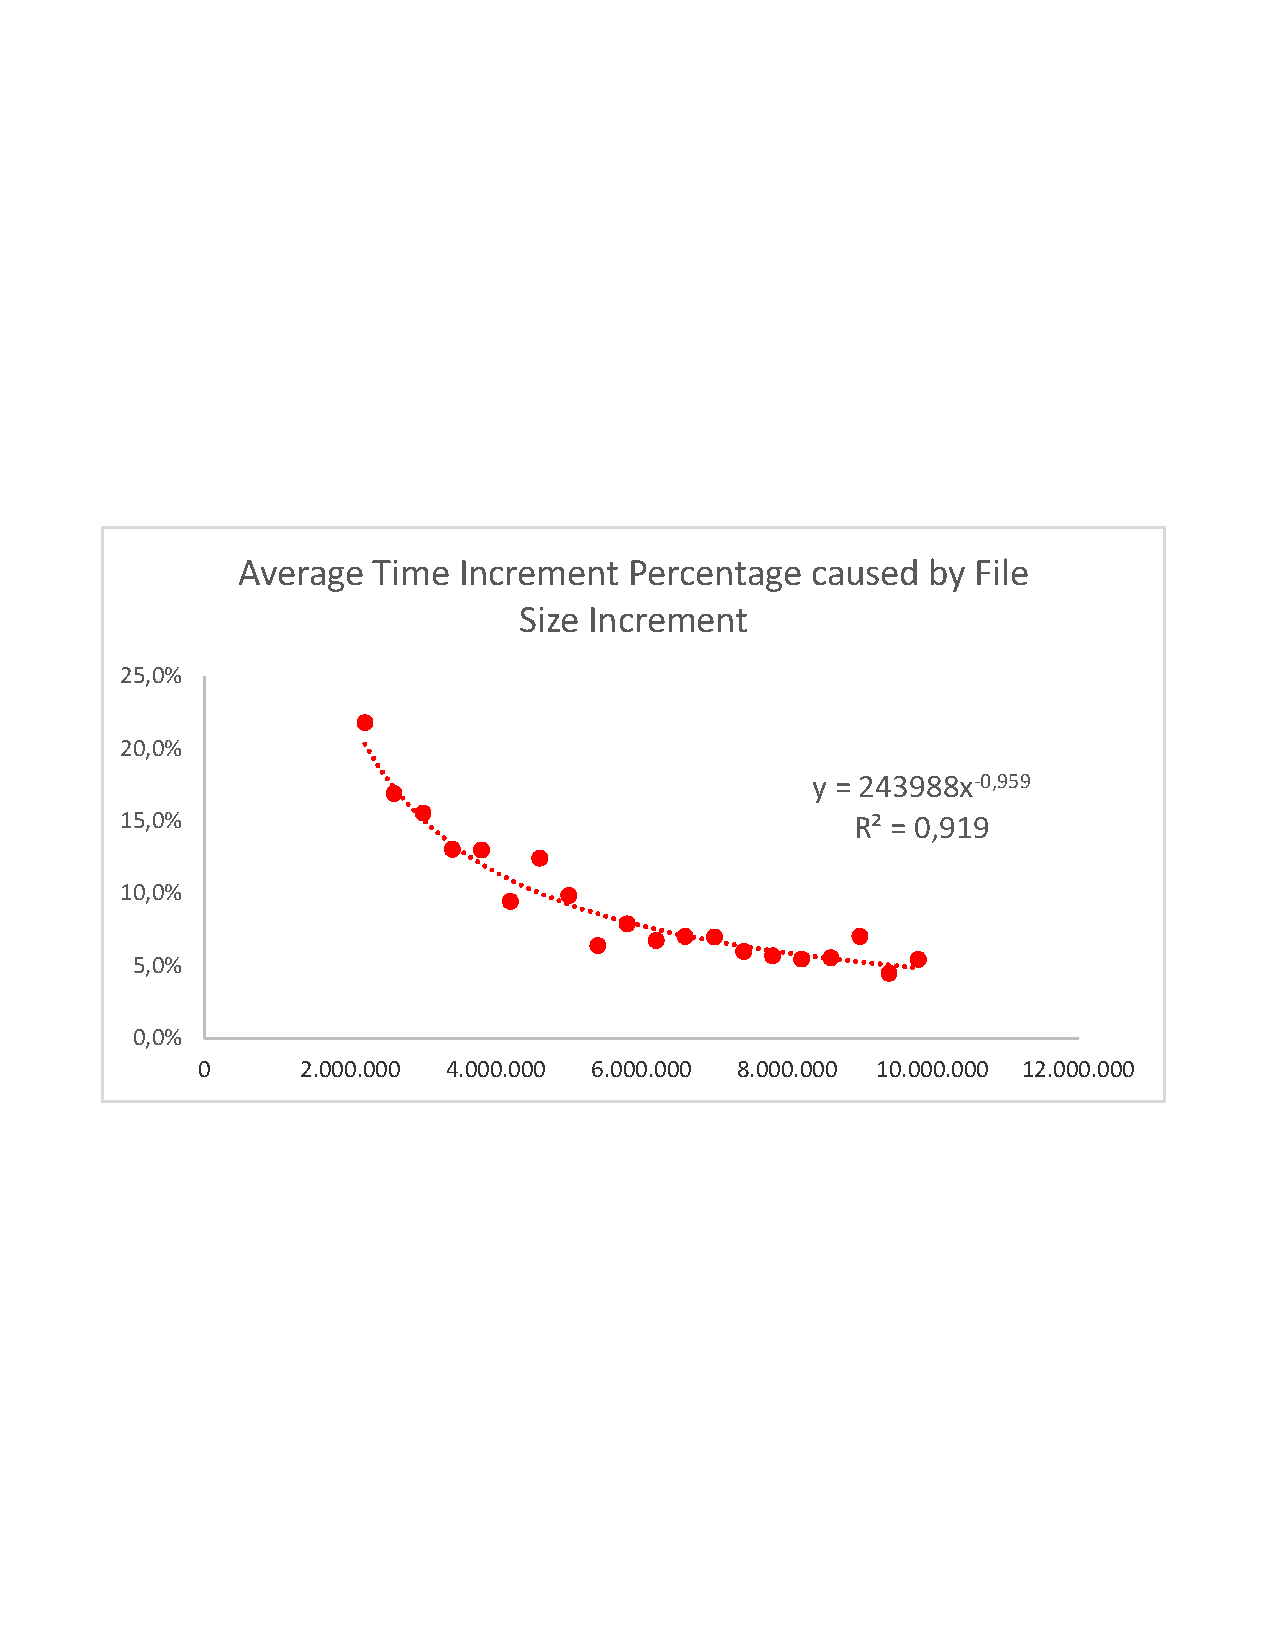
\includegraphics[trim=0cm 8.5cm -1cm 10cm, scale=0.8]{fig/fileSize.eps}
		\caption{Average Time Increment Percentage caused by File Size Increment}
		\label{fig:fileSize}
	\end{figure}

We can think that because the file size impacts each time minus the total time to process the file our proposed architectures could try to process files each time bigger. It could help us to know the limit of processing of our design patterns.

\subsection{Processing Nodes Analysis}
\label{subsec:processingNodesAnalysis}
Available processing nodes variable data was consolidated in table \ref{tab:improvementAvailableNodes}. We can observe that improvement caused by increasing the number of available nodes is not linear, that is, it does not occur that when the number available nodes are increasing the system performance is improved. By contrast, the improvement is smallest while more nodes are added. Additionally, the structure memory variable impacts the improvement achieved. Table \ref{tab:improvementAvailableNodes} shows that the Norma average improvement is smallest than the Uma memory structure. The figure \ref{fig:availableNodes} show an approximation logarithmic equation that adjusts to the behavior of the improvement percentage when the available nodes are increased.

We relate this behavior to communication time behavior. Table \ref{tab:communicationTimePercentage} summarizes the communication time percentage on the total processing time, it is worth noting that the Uma memory structure data includes the read phase time as part of the communication time, while the Norma memory structure does not. In this table is evident that the communication time percentage increases as the number available nodes increase too. 

% Please add the following required packages to your document preamble:
% \usepackage{multirow}
% \usepackage{graphicx}
\begin{table}[]
	\centering
	\caption{Average of the Improvement Percentage by Increasing Available Nodes}
	\label{tab:improvementAvailableNodes}
	\resizebox{\textwidth}{!}{%
			\begin{tabular}{|c|c|c|c|c|c|c|c|c|c|c|c|c|}
				\hline
				\multirow{2}{*}{\begin{tabular}[c]{@{}c@{}}MEMORY \\ STRUCTURE\end{tabular}} & \multirow{2}{*}{\begin{tabular}[c]{@{}c@{}}DESIGN \\ PATTERN\end{tabular}} & \multicolumn{4}{c|}{RMI (\%)} & \multicolumn{3}{c|}{REST (\%)} & \multicolumn{4}{c|}{ICE (\%)} \\ \cline{3-13} 
				&  & 2 & 4 & 8 & 16 & 2 & 4 & 8 & 2 & 4 & 8 & 16 \\ \hline
				\multirow{4}{*}{NORMA} & Original Strategy Variation & 10,23 & 6,79 & 1,35 & -2,16 & 24,74 & -2,77 & -3,95 & 8,92 & 9,64 & -1,90 & -11,24 \\ \cline{2-13} 
				& Fork/Join Java library & 16,43 & 3,00 & -5,20 & -2,58 & 20,61 & -8,26 & -4,95 & 6,49 & 1,80 & -8,74 & -8,25 \\ \cline{2-13} 
				& Fork-Join Design Pattern & 29,25 & 22,65 & 2,00 & 2,19 & 36,37 & 18,71 & 7,05 & 44,25 & 38,49 & 17,96 & 5,13 \\ \cline{2-13} 
				& Leader-Followers Design Pattern & -0,15 & -1,00 & -0,95 & -1,47 & -2,20 & -3,11 & -0,85 & -7,36 & -1,36 & -0,79 & -3,52 \\ \hline
				\multicolumn{2}{|c|}{NORMA AVERAGE} & 13,94 & 7,86 & -0,70 & -1,00 & 19,88 & 1,14 & -0,68 & 13,07 & 12,14 & 1,63 & -4,47 \\ \hline
				\multirow{5}{*}{UMA} & Original Strategy Variation & 37,58 & 26,36 & 1,71 & -1,02 & 49,82 & 30,94 & 1,53 & 24,82 & 22,62 & 4,50 & -9,69 \\ \cline{2-13} 
				& Fork/Join Java library & 39,23 & 20,98 & -1,56 & -19,02 & 44,73 & 16,21 & 2,23 & 7,37 & 15,88 & 1,19 & -7,57 \\ \cline{2-13} 
				& Fork-Join Design Pattern & 57,45 & 27,76 & 18,17 & -5,85 & 68,18 & 30,11 & 16,08 & 63,12 & 47,28 & 24,25 & 9,76 \\ \cline{2-13} 
				& Original Strategy & 10,49 & -0,91 & -4,08 & -4,55 & 10,50 & 5,74 & -4,48 & 13,99 & 8,17 & 4,32 & -4,55 \\ \cline{2-13} 
				& Leader-Followers Design Pattern & -7,00 & 4,11 & -3,52 & -2,09 & -8,51 & 2,67 & 0,48 & 9,21 & -0,92 & -3,04 & 11,15 \\ \hline
				\multicolumn{2}{|c|}{UMA AVERAGE} & 27,55 & 15,66 & 2,14 & -6,51 & 32,95 & 17,14 & 3,17 & 23,70 & 18,61 & 6,24 & -0,18 \\ \hline
				\multicolumn{2}{|c|}{AVERAGE} & 21,50 & 12,19 & 0,88 & -4,06 & 27,14 & 10,03 & 1,46 & 18,98 & 15,73 & 4,19 & -2,09 \\ \hline
			\end{tabular}%
		}
	\end{table}
	
	\begin{figure}
		\centering
		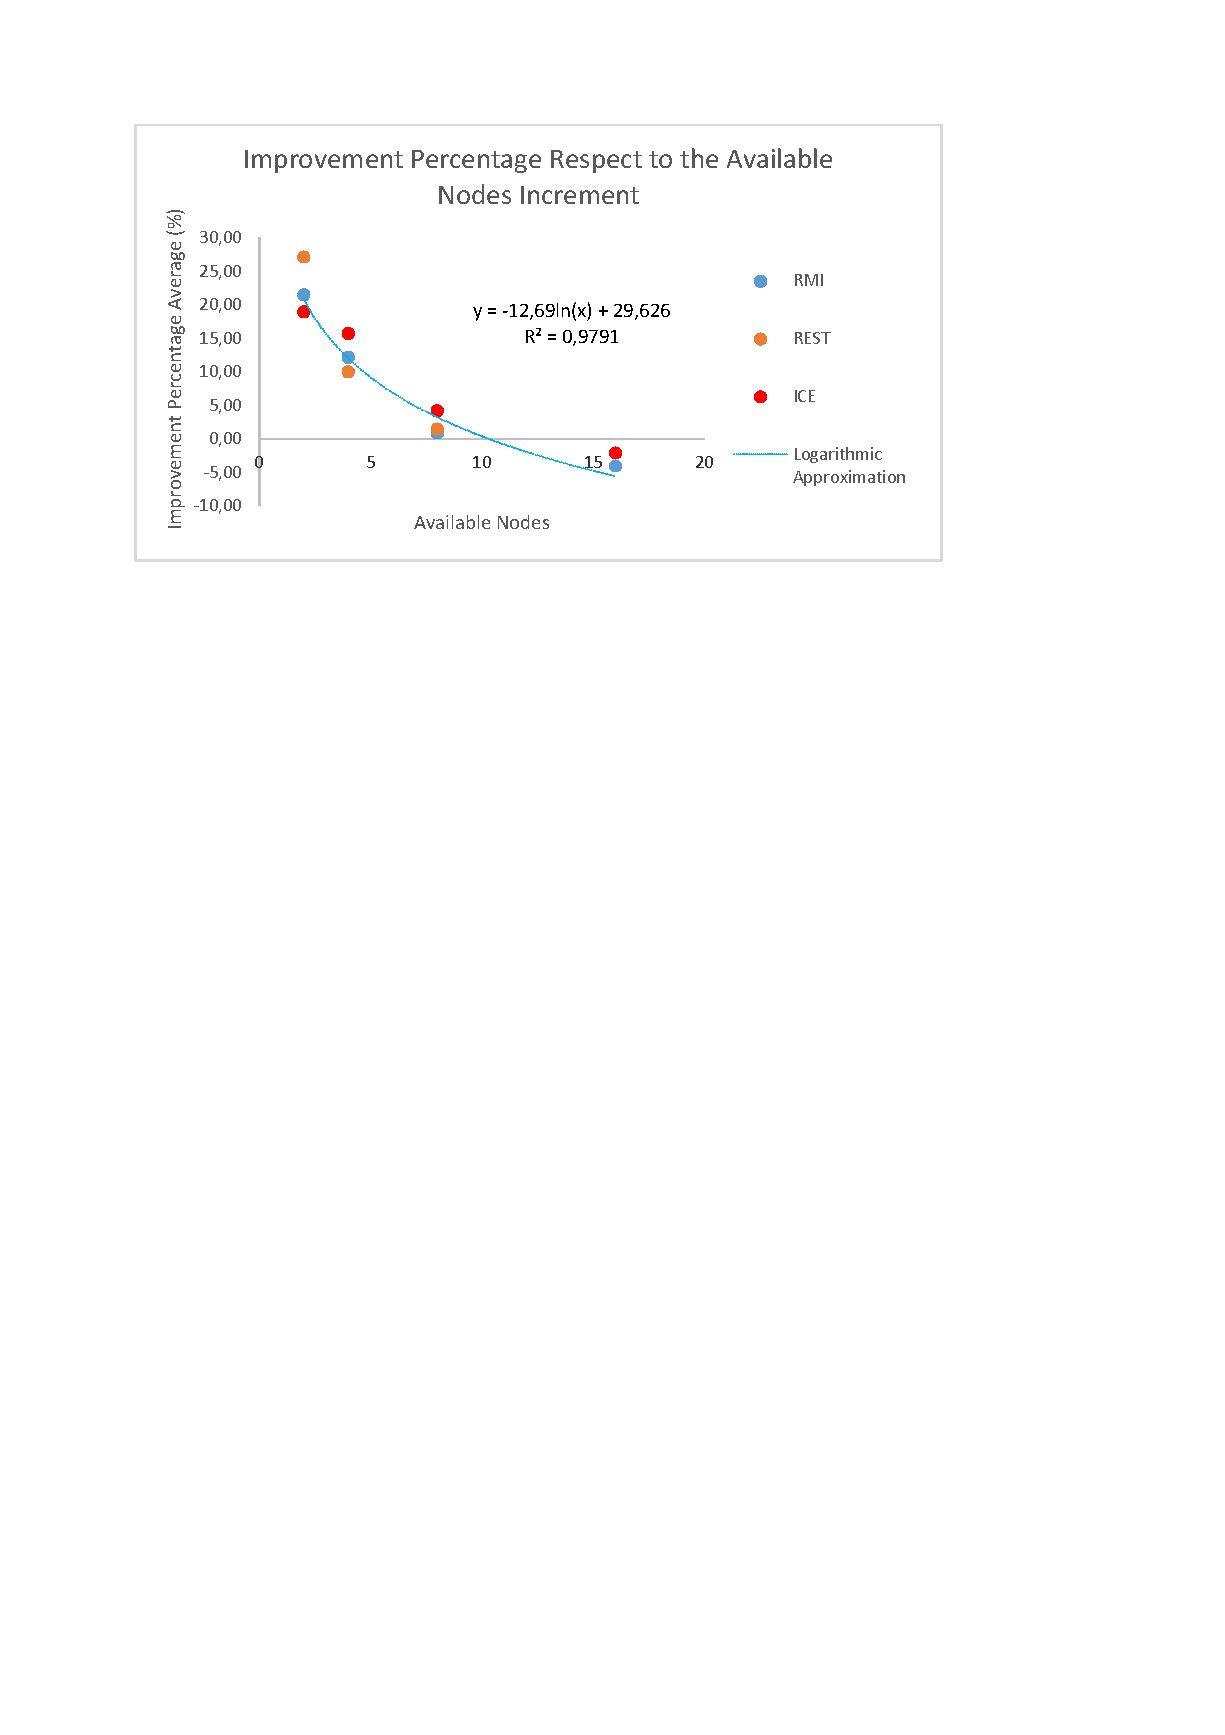
\includegraphics[trim=0.5cm 19cm 1cm 1cm]{fig/availableNodes.eps}
		\caption{Improvement Percentage Respect to the Available Nodes Increment}
		\label{fig:availableNodes}
	\end{figure}

\subsection{Communication Protocol Analysis}
According to the chart \ref{fig:betterTimesCommunicationProtocol} Ice is the best communication protocol among the studied protocols. The protocols Rest and RMI were implemented over the FraSCAti middleware and this middleware could be a factor that influence this result. 

Currently, Rest is a very used protocol due to it allows us to inter-operate among different software systems, but, if you are searching for more performance for your application you should evaluate to use another alternative such as Ice. \\
%Make Graphics comparisonCommunicationProtocols.eps betterTimesCommunicationProtocol.eps

If we compare the performance of communication protocols in pairs such as in the chart \ref{fig:comparisonCommunicationProtocols}, we can observe that if we only compare Rest vs Rmi, Rest has a better performance in 60\% times. This says to us that although Rmi in the whole experiment has a bigger amount of test with more performance (10,34\%), Rest could have better performance than RMI if we have only these two options.
\begin{figure}[H]
	\centering
	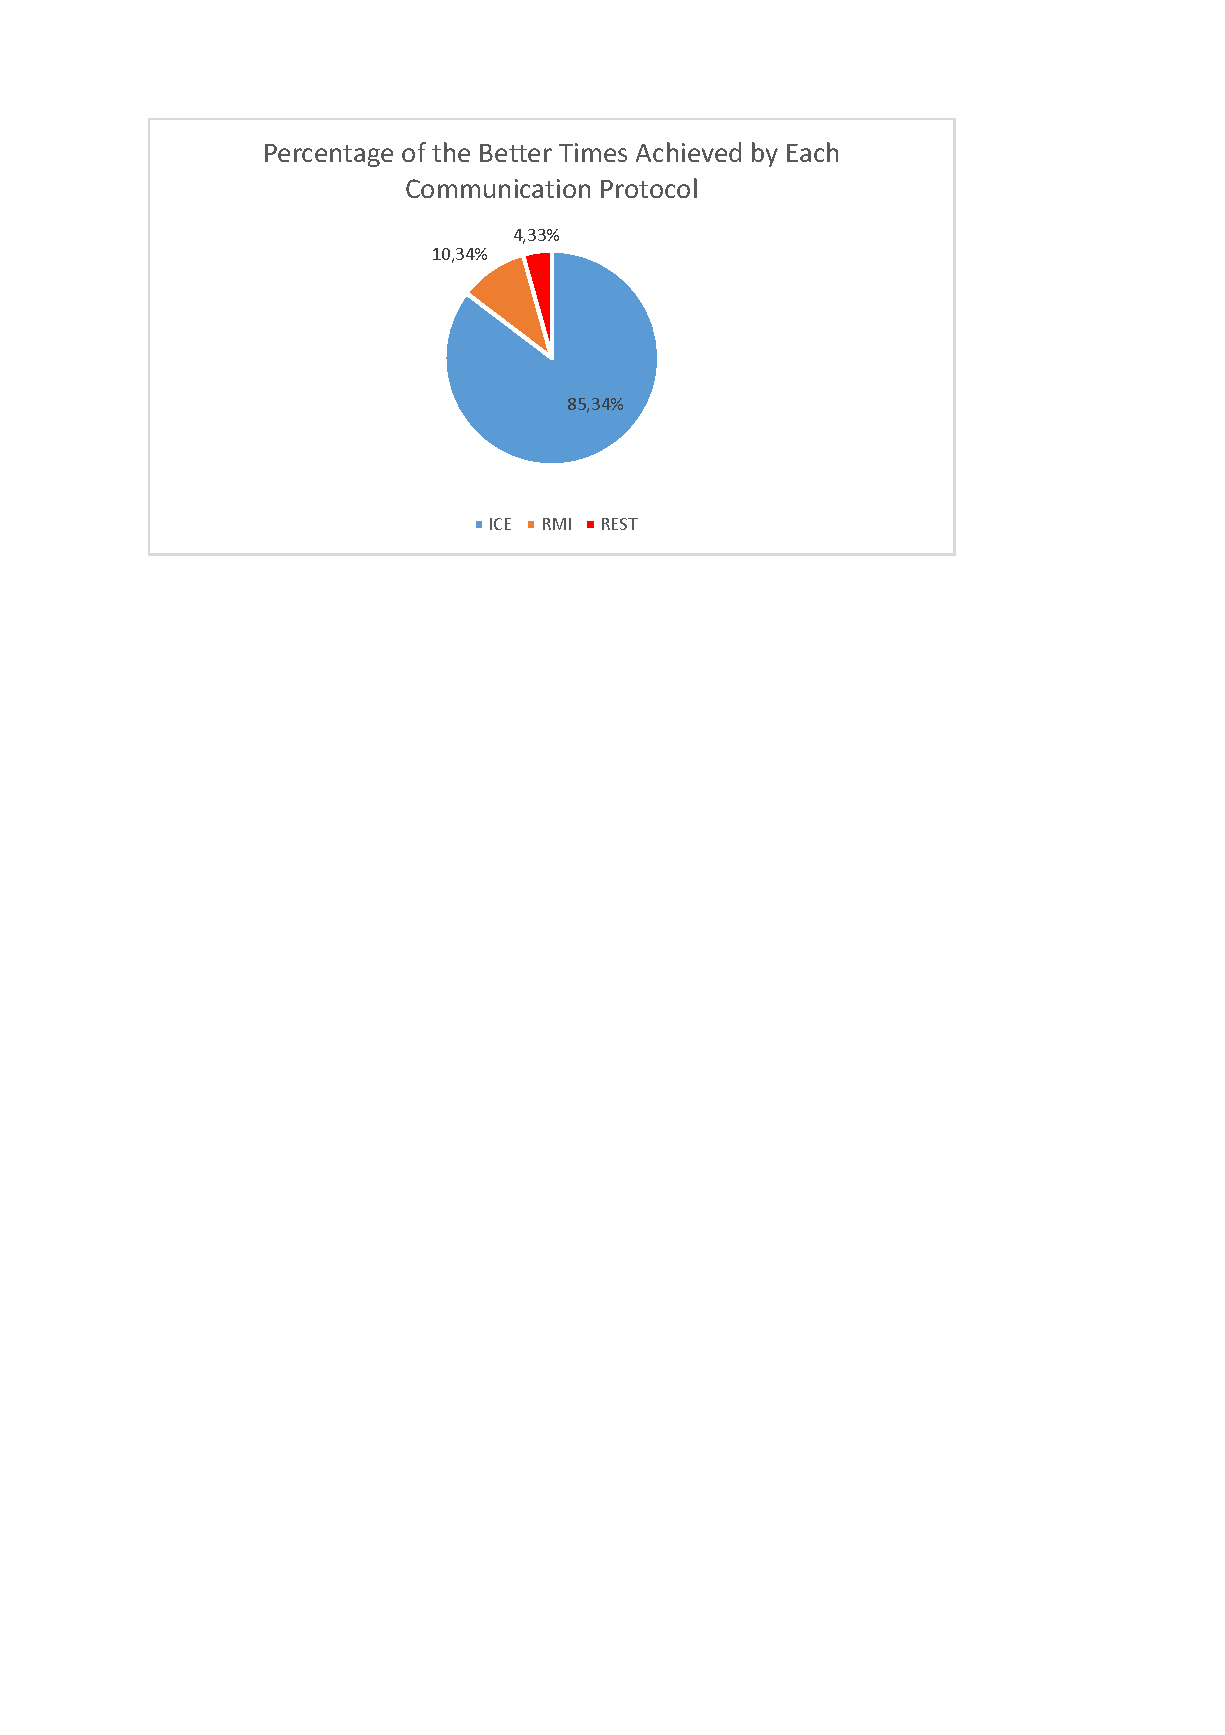
\includegraphics[trim=0.5cm 19cm 1cm 1cm]{fig/betterTimesCommunicationProtocol.eps}
	\caption{Percentage of the Better Times Achieved by Each Communication Protocol}
	\label{fig:betterTimesCommunicationProtocol}
\end{figure}

\begin{figure}[H]
	\centering
	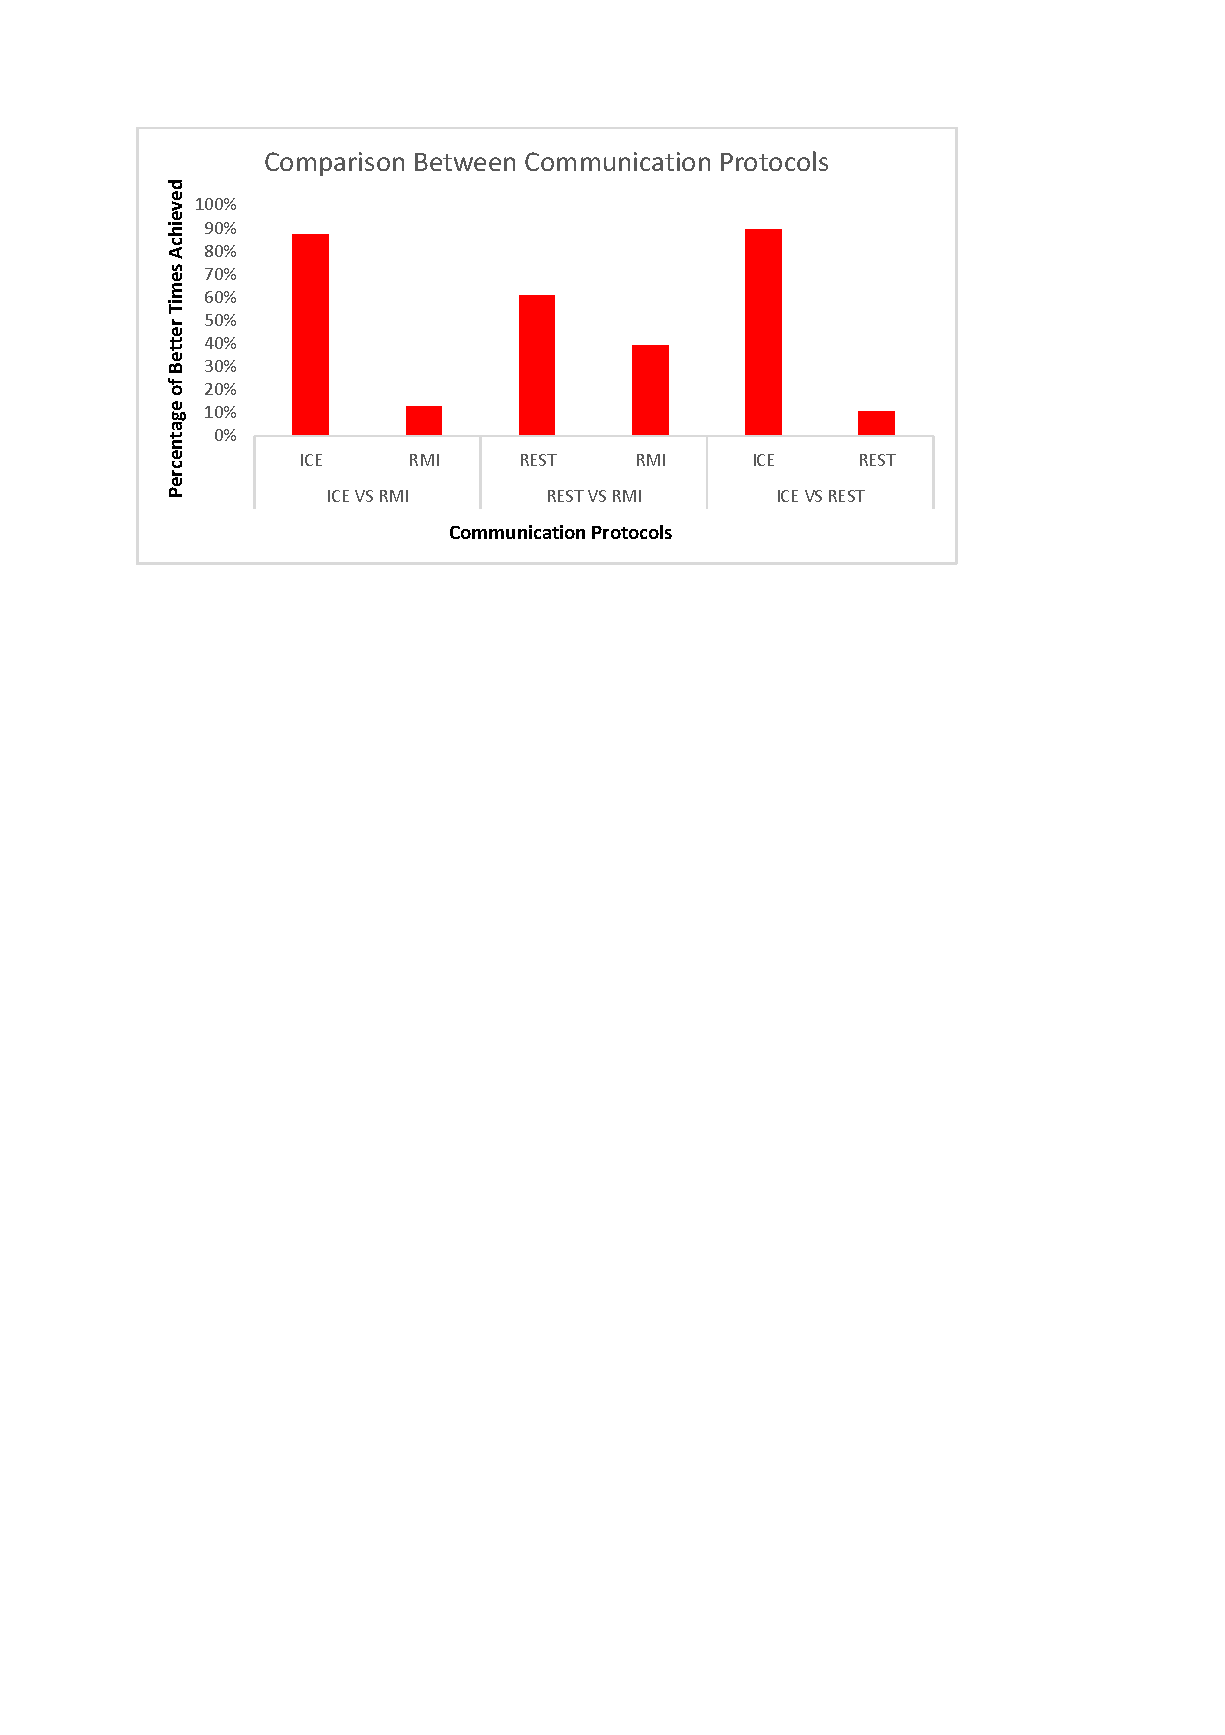
\includegraphics[trim=0.5cm 19cm 1cm 1cm]{fig/comparisonCommunicationProtocols.eps}
	\caption{Comparison Between Communication Protocols}
	\label{fig:comparisonCommunicationProtocols}
\end{figure}

\subsection{Memory Structure Analysis}
\label{subsec:memoryAnalysis}

When we start the memory analysis the first conclusion that is evident is that UMA is the best memory configuration if we are searching for the best performance. UMA has pros y cons at the same that NORMA, but the more important consideration is the bottleneck that this configuration could have. Table \ref{tab:memoryAverage} shows the percentage of times that UMA was better than NORMA. When Ice is the communication protocol UMA always is better than NORMA in more than 60\% of cases.  

% Please add the following required packages to your document preamble:
% \usepackage{multirow}
% \usepackage{graphicx}
\begin{table}[H]
	\centering
	\caption{Average of the Total Time Percentage of the Uma Memory Structure Respect to the Norma Memory Structure.}
	\label{tab:memoryAverage}
%	\resizebox{\textwidth}{!}{%
		\begin{tabular}{|c|c|c|}
			\hline
			\begin{tabular}[c]{@{}c@{}}Communication\\  Protocol\end{tabular} & \begin{tabular}[c]{@{}c@{}}Design\\  Pattern\end{tabular} & Average \\ \hline
			\multirow{4}{*}{RMI} & \begin{tabular}[c]{@{}c@{}}Original Strategy \\ Variation\end{tabular} & 47,9\% \\ \cline{2-3} 
			& \begin{tabular}[c]{@{}c@{}}Fork/Join\\ Java library\end{tabular} & 44,6\% \\ \cline{2-3} 
			& \begin{tabular}[c]{@{}c@{}}Fork-Join\\  Design Pattern\end{tabular} & 62,2\% \\ \cline{2-3} 
			& \begin{tabular}[c]{@{}c@{}}Leader-Followers \\ Design Pattern\end{tabular} & 63,4\% \\ \hline
			\multirow{4}{*}{REST} & \begin{tabular}[c]{@{}c@{}}Original Strategy\\  Variation\end{tabular} & 44,4\% \\ \cline{2-3} 
			& \begin{tabular}[c]{@{}c@{}}Fork/Join\\ Java library\end{tabular} & 45,6\% \\ \cline{2-3} 
			& \begin{tabular}[c]{@{}c@{}}Fork-Join\\  Design Pattern\end{tabular} & 64,9\% \\ \cline{2-3} 
			& \begin{tabular}[c]{@{}c@{}}Leader-Followers\\  Design Pattern\end{tabular} & 64,1\% \\ \hline
			\multirow{4}{*}{ICE} & \begin{tabular}[c]{@{}c@{}}Original Strategy\\  Variation\end{tabular} & 65,4\% \\ \cline{2-3} 
			& \begin{tabular}[c]{@{}c@{}}Fork/Join\\ Java library\end{tabular} & 60,6\% \\ \cline{2-3} 
			& \begin{tabular}[c]{@{}c@{}}Fork-Join \\ Design Pattern\end{tabular} & 85,9\% \\ \cline{2-3} 
			& \begin{tabular}[c]{@{}c@{}}Leader-Followers\\  Design Pattern\end{tabular} & 60,7\% \\ \hline
		\end{tabular}%
%	}
\end{table}

In Rest and RMI, UMA is better than NORMA in more than 60\% of cases only for the Fork-Join and Leader/Followers design patterns and in more than 40\% of times for the Original Strategy Variation and the Fork-Join Java Library. It looks like the last strategies could generate a bottleneck before the other strategies. This behaviour could be justified due to the Fork-Join and the Leader-Followers design patterns send the tasks to their processing units and these can process from that moment (i.e. a structure more horizontal), but another design patterns use a structure more hierarchical.


Due to the consistent behavior observed in this variable, we try to generate a statistical model that can predict its behavior. We try a linear regression and the ANOVA, in the tables \ref {tab:regressionStatistics} and \ref {tab:regressionStatisticsData} we summarize the results obtained. First, we can see that based on the coefficient of determination (R2) and the adjusted coefficient of determination (adjusted R2) this model is not the best to represent the behavior of memory structure. These coefficients of determination are indicators between the range 1-0, the closer to 1 the better the model, and we have 0,425 and 0,423 respectively. Second, we have multifactorial ANOVA. This model considers the effect of each studied variable and according to the P-value indicator, this is a good model to predict the structure memory variable. The P-value is used to validate the hypothesis proposed, the proposed hypothesis says that for each variable, it is significant to construct the model of the memory structure. If the calculated P-value of the variable is less than 0,05 so, the variable is accepted for the model.

\begin{table}[H]
	\centering
	\caption{Regression Statistics}
	\label{tab:regressionStatistics}
	\begin{tabular}{|l|l|}
		\hline
		Multiple R & 0,652070218 \\ \hline
		R Square & 0,425195569 \\ \hline
		Adjusted R Square & 0,423060733 \\ \hline
		Standard Error & 0,111858357 \\ \hline
		Observations & 1082 \\ \hline
	\end{tabular}
\end{table}

\begin{table}[H]
	\centering
	\caption{Regression Statistics Data}
	\label{tab:regressionStatisticsData}
	\resizebox{\textwidth}{!} & \textit{Upper 95\%} & \textit{Lower 95,0\%} & \textit{Upper 95,0\%} \\ \hline
			Intercept & 0,384230933 & 0,014801709 & 25,95855285 & 8,9435E-116 & 0,355187478 & 0,413274387 & 0,355187478 & 0,413274387 \\ \hline
			\begin{tabular}[c]{@{}c@{}}File \\ Size\end{tabular} & -6,91906E-09 & 1,40333E-09 & -4,930466112 & 9,49415E-07 & -9,67262E-09 & -4,16549E-09 & -9,67262E-09 & -4,16549E-09 \\ \hline
			\begin{tabular}[c]{@{}c@{}}Available \\ Nodes\end{tabular} & -0,007141392 & 0,000706497 & -10,10816596 & 5,19951E-23 & -0,008527659 & -0,005755125 & -0,008527659 & -0,005755125 \\ \hline
			\begin{tabular}[c]{@{}c@{}}Design \\ Pattern\end{tabular} & 0,05680204 & 0,00317531 & 17,88865847 & 7,30488E-63 & 0,050571544 & 0,063032535 & 0,050571544 & 0,063032535 \\ \hline
			\begin{tabular}[c]{@{}c@{}}Communication \\ Protocol\end{tabular} & 0,076994391 & 0,003991936 & 19,28748296 & 1,95675E-71 & 0,069161538 & 0,084827244 & 0,069161538 & 0,084827244 \\ \hline
		\end{tabular}%
	}
\end{table}

Thus, the formula that predicts the memory structure behavior is showed in the equation \ref{eq:memory}.

\begin{equation}
\label{eq:memory}
\resizebox{.92\hsize}{!}{$Uma Respect Norma = 0,384230933 - 6,91905547282634E^{-09}(fs) - 0,00714139220840687(n) + 0,0568020397510634(dp) + 0,0769943910761448(cp)$}
\end{equation} 

\subsection{Bandwidth Analysis}
\label{subsec:bandwidthAnalysis}
% Please add the following required packages to your document preamble:
% \usepackage{multirow}
% \usepackage{graphicx}

The bandwidth variable was tested using two values, 100MB and 1GB. Table \ref{tab:consolidatedData100MB} summarizes the times that each one of these tests takes with a configuration of 100MB. When we compare these tests with the same configuration executed at 1GB (reference section \ref{sebsec:consolidatedData}) we can verify that the relation between them is approximately 10 times. Table \ref{tab:calculatedRelation} summarizes this information. 

\begin{table}[H]
	\label{tab:consolidatedData100MB}
	\fontsize{16}{36}\selectfont
	\centering
	\begin{center}
		\caption{Consolidated Data of the Experiments with Bandwidth Configuration of 100MB}
	\end{center}
	\resizebox{\textwidth}{!}{%
		\begin{tabular}{|c|c|c|c|c|c|c|c|c|c|c|c|c|c|c|c|c|c|c|c|c|c|}
			\hline
			\multirow{4}{*}{File Size} & \multicolumn{13}{c|}{ICE} & \multicolumn{2}{c|}{RMI} & \multicolumn{6}{c|}{REST} \\ \cline{2-22} 
			& \multicolumn{7}{c|}{Fork/Join Java library (ms)} & \multicolumn{3}{c|}{\begin{tabular}[c]{@{}c@{}}Variant of Original \\ Strategy - Separation\\ of Merge Component\\  (ms)\end{tabular}} & \multicolumn{3}{c|}{\begin{tabular}[c]{@{}c@{}}Original\\  Strategy \\ (ms)\end{tabular}} & \begin{tabular}[c]{@{}c@{}}Original\\ Strategy\\ (ms)\end{tabular} & \begin{tabular}[c]{@{}c@{}}Fork/Join\\ Java\\ library\\ (ms)\end{tabular} & \multicolumn{3}{c|}{\begin{tabular}[c]{@{}c@{}}Original \\ Strategy \\ (ms)\end{tabular}} & \multicolumn{3}{c|}{\begin{tabular}[c]{@{}c@{}}Fork/Join \\ Java library \\ (ms)\end{tabular}} \\ \cline{2-22} 
			& \multicolumn{4}{c|}{UMA} & \multicolumn{3}{c|}{NORMA} & \multicolumn{3}{c|}{UMA} & \multicolumn{3}{c|}{UMA} & UMA & NORMA & \multicolumn{3}{c|}{UMA} & \multicolumn{3}{c|}{NORMA} \\ \cline{2-22} 
			& 2 & 4 & 8 & 16 & 2 & 4 & 8 & 2 & 4 & 8 & 2 & 4 & 8 & 2 & 2 & 2 & 4 & 8 & 2 & 4 & 8 \\ \hline
			1.800.000 & 16970,1 & 15747,4 & 16733,7 & 17388,7 & 29793,3 & 36149,5 & 40443,3 & 15896,7 & 18999,8 & 17262,9 & 17571,4 & 20704,5 & 21963,4 & 22247,5 & 36675,2 & 33466,7 & 36550,0 & 40886,3 & 55660,1 & 70549,5 & 76135,3 \\ \hline
			2.600.000 & 26006,9 & 22744,6 & 22814,6 & 24181,8 & 45621,2 & 53643,7 & 55298,5 & 26367,1 & 26774,8 & 24957,6 & 25699,9 & 29028,6 & 32459,2 & 27127,4 & 53819,9 & 41573,8 & 54247,3 & 56516,4 & 85747,8 & 100979,9 & 111670,8 \\ \hline
			3.400.000 & 31183,4 & 29276,5 & 32671,9 & 31612,3 & 59213,8 & 67254,1 & 77418,1 & 29368,9 & 34714,3 & 32498,1 & 30343,7 & 38117,7 & 41593,0 & 39617,0 & 69648,2 & 61099,4 & 72217,7 & 76444,5 & 108606,5 & 136715,9 & 145883,6 \\ \hline
			4.200.000 & 38727,3 & 35737,9 & 39156,8 & 38823,6 & 72797,2 & 83911,4 & 89244,4 & 43189,2 & 42182,2 & 38737,6 & 35171,0 & 49083,4 & 51904,5 & 43854,5 & 85884,3 & 78947,9 & 83770,1 & 94894,8 & 137490,8 & 167252,0 & 171630,6 \\ \hline
			5.000.000 & 49180,3 & 42478,2 & 44179,1 & 45303,9 & 88363,8 & 97659,8 & 107022,1 & 46358,1 & 50815,6 & 48795,8 & 47591,4 & 59010,7 & 62616,9 & 58106,6 & 102930,3 & 89540,4 & 106118,6 & 107609,2 & 164964,1 & 196633,3 & 208206,1 \\ \hline
			5.800.000 & 49638,7 & 47949,6 & 51454,8 & 53385,4 & 102717,2 & 113744,5 & 127881,3 & 49469,3 & 57357,9 & 53391,6 & 62038,6 & 72011,7 & 74578,6 & 71724,4 & 120358,9 & 105688,6 & 116799,6 & 129974,6 & 190453,4 & 226992,1 & 237022,9 \\ \hline
			6.600.000 & 64909,7 & 55185,6 & 56940,3 & 59266,2 & 114018,8 & 135523,5 & 144413,2 & 58269,6 & 65735,4 & 61453,0 & 74653,0 & 82121,4 & 83089,6 & 84936,3 & 136892,5 & 118800,9 & 132164,7 & 139593,1 & 213139,5 & 253192,4 & 271693,9 \\ \hline
			7.400.000 & 80608,3 & 61799,1 & 71178,6 & 61254,3 & 128554,8 & 149762,6 & 163666,9 & 64606,7 & 62190,5 & 61319,3 & 72340,8 & 91748,9 & 91536,8 & 86990,0 & 150728,7 & 136771,9 & 157942,8 & 167403,6 & 233717,2 & 280386,0 & 304656,0 \\ \hline
			8.200.000 & 80140,7 & 67168,1 & 68911,9 & 63599,1 & 143736,0 & 165548,9 & 183593,2 & 64297,8 & 66238,3 & 64932,1 & 82694,6 & 99219,1 & 102337,8 & 96738,4 & 165349,8 & 151335,0 & 173249,2 & 185856,1 & 253746,8 & 294756,0 & 334041,2 \\ \hline
			9.000.000 & 87568,2 & 73701,5 & 85696,4 & 65368,4 & 151172,4 & 178378,7 & 195318,8 & 81253,0 & 73178,6 & 74544,1 & 95440,5 & 108975,3 & 111142,9 & 109300,5 & 184773,3 & 166631,2 & 191875,7 & 203211,4 & 272457,2 & 312547,0 & 371181,20 \\ \hline
			9.800.000 & 112357,9 & 79198,3 & 93441,6 & 69357,2 & 153318,7 & 198253,3 & 216476,0 & 96881,4 & 77039,4 & 76023,6 & 95300,4 & 115636,6 & 119476,6 & 124941,1 & 203612,9 & 184412,0 & 211208,8 & 217854,3 & 297805,8 & 334752,0 & 394521,4 \\ \hline
		\end{tabular}%
	}
\end{table}


% Please add the following required packages to your document preamble:
% \usepackage{multirow}
% \usepackage{graphicx}
\begin{table}[H]
	\fontsize{12}{24}\selectfont
	\centering
	\caption{Calculated relation among the Experiments with Bandwidth Configuration of 100MB and 1GB}
	\label{tab:calculatedRelation}
	\resizebox{\textwidth}{!}{%
		\begin{tabular}{|c|c|c|c|c|c|c|c|c|c|c|c|c|c|c|c|c|c|c|c|l|l|}
			\hline
			\multirow{4}{*}{File Size} & \multicolumn{13}{c|}{ICE} & \multicolumn{2}{c|}{RMI} & \multicolumn{6}{c|}{REST} \\ \cline{2-22} 
			& \multicolumn{7}{c|}{Fork/Join Java library (ms)} & \multicolumn{3}{c|}{\begin{tabular}[c]{@{}c@{}}Variant of Original\\ Strategy -Separation\\ of Merge Component \\  (ms)\end{tabular}} & \multicolumn{3}{c|}{\begin{tabular}[c]{@{}c@{}}Original \\ Strategy \\ (ms)\end{tabular}} & \begin{tabular}[c]{@{}c@{}}Original\\ Strategy \\ (ms)\end{tabular} & \begin{tabular}[c]{@{}c@{}}Fork/Join\\ Java\\ library\\ (ms)\end{tabular} & \multicolumn{3}{c|}{\begin{tabular}[c]{@{}c@{}}Original \\ Strategy\\  (ms)\end{tabular}} & \multicolumn{3}{c|}{\begin{tabular}[c]{@{}c@{}}Fork/Join\\  Java library\\  (ms)\end{tabular}} \\ \cline{2-22} 
			& \multicolumn{4}{c|}{UMA} & \multicolumn{3}{c|}{NORMA} & \multicolumn{3}{c|}{UMA} & \multicolumn{3}{c|}{UMA} & UMA & NORMA & \multicolumn{3}{c|}{UMA} & \multicolumn{3}{c|}{NORMA} \\ \cline{2-22} 
			& 2 & 4 & 8 & 16 & 2 & 4 & 8 & 2 & 4 & 8 & 2 & 4 & 8 & 2 & 2 & 2 & 4 & 8 & 2 & 4 & 8 \\ \hline
			1.800.000 & 6,43 & 6,44 & 7,08 & 6,90 & 8,74 & 9,95 & 11,41 & 6,45 & 8,78 & 8,20 & 9,55 & 11,87 & 12,88 & 9,31 & 7,19 & 14,03 & 15,08 & 16,07 & 10,21 & 12,34 & 13,13 \\ \hline
			2.600.000 & 8,40 & 8,10 & 8,44 & 8,45 & 9,12 & 11,64 & 10,68 & 8,62 & 10,29 & 9,90 & 9,93 & 11,00 & 13,71 & 7,47 & 7,29 & 12,65 & 16,30 & 15,18 & 11,94 & 13,78 & 11,78 \\ \hline
			3.400.000 & 8,22 & 8,97 & 10,70 & 9,06 & 10,90 & 10,93 & 14,77 & 7,85 & 11,30 & 10,92 & 7,68 & 10,34 & 11,20 & 8,44 & 7,81 & 14,49 & 16,58 & 15,94 & 11,94 & 14,20 & 12,66 \\ \hline
			4.200.000 & 9,13 & 9,77 & 9,58 & 8,58 & 11,23 & 12,49 & 13,23 & 9,82 & 11,59 & 10,83 & 7,28 & 10,89 & 11,75 & 7,53 & 7,06 & 14,18 & 15,43 & 16,08 & 12,52 & 12,76 & 13,03 \\ \hline
			5.000.000 & 10,32 & 10,50 & 9,81 & 9,50 & 12,09 & 12,79 & 12,69 & 8,11 & 10,18 & 10,12 & 8,32 & 11,13 & 11,90 & 7,98 & 6,51 & 13,99 & 16,49 & 16,76 & 12,63 & 13,43 & 13,15 \\ \hline
			5.800.000 & 8,44 & 9,08 & 10,19 & 10,12 & 12,52 & 14,61 & 13,53 & 7,12 & 10,51 & 10,16 & 9,07 & 11,60 & 12,57 & 8,08 & 6,54 & 13,68 & 14,79 & 18,66 & 12,77 & 12,39 & 13,66 \\ \hline
			6.600.000 & 10,26 & 9,90 & 10,61 & 10,35 & 12,61 & 15,64 & 14,13 & 8,07 & 11,15 & 10,86 & 9,80 & 11,92 & 12,43 & 8,50 & 6,30 & 13,11 & 14,89 & 15,56 & 12,38 & 12,62 & 12,34 \\ \hline
			7.400.000 & 11,95 & 10,36 & 12,54 & 9,77 & 12,81 & 15,95 & 14,99 & 8,21 & 9,78 & 10,10 & 8,50 & 11,83 & 12,42 & 7,86 & 5,95 & 12,21 & 17,04 & 16,26 & 10,50 & 11,07 & 12,20 \\ \hline
			8.200.000 & 9,97 & 10,58 & 11,26 & 8,73 & 12,45 & 16,21 & 15,36 & 7,05 & 9,75 & 10,14 & 8,59 & 11,66 & 12,67 & 7,75 & 5,91 & 12,57 & 15,03 & 16,30 & 9,30 & 10,12 & 11,95 \\ \hline
			9.000.000 & 10,41 & 10,93 & 13,29 & 8,69 & 11,38 & 12,66 & 13,72 & 8,00 & 8,91 & 10,47 & 9,37 & 11,71 & 12,54 & 7,41 & 5,58 & 11,72 & 16,83 & 16,85 & 9,40 & 10,93 & 12,02 \\ \hline
			9.800.000 & 12,51 & 11,28 & 12,35 & 11,8 & 10,76 & 13,68 & 13,29 & 8,98 & 8,84 & 9,16 & 8,49 & 11,48 & 12,55 & 7,72 & 5,63 & 12,64 & 15,41 & 15,41 & 10,04 & 10,38 & 11,24 \\ \hline
		\end{tabular}%
	}
\end{table}


\subsection{General Design Patterns Analysis}
\label{subsec:designPatternsAnalysis}

The table \ref{tab:designPatternsCom} summarizes the times that each design pattern has the best processing time. The design pattern with more best processing times is the Fork/Join Java library, it has 275 times. The worse design pattern is the Fork/Join Design Pattern, it has 18 times.

This result is very interesting due to the worse result was gotten with the distributed version of the Fork/Join Java Library. We can think that we should improve the code implementation or the strategy used to extrapolate the design pattern to a distributed environment. That is why we analyze the results gotten discriminated against by each studied variable.

% Please add the following required packages to your document preamble:
% \usepackage{multirow}
\begin{table}[H]
\centering
	\caption{Design Patterns Comparision}
	\label{tab:designPatternsCom}
	\resizebox{\textwidth}{!}{%
\begin{tabular}{|l|c|c|c|c|c|c|c|c|c|c|c|c|c|c|c|c|c|c|}
\hline
\multicolumn{1}{|c|}{\multirow{2}{*}{\textbf{Design Patterns}}} &
  \multirow{2}{*}{\textbf{Total Count}} &
  \multicolumn{2}{c|}{\textbf{Memory Structure}} &
  \multicolumn{3}{c|}{\textbf{Communication Protocols}} &
  \multicolumn{5}{c|}{\textbf{Processing Nodes}} &
  \multicolumn{7}{c|}{\textbf{File Size}} \\ \cline{3-19} 
\multicolumn{1}{|c|}{} &
   &
  \textbf{Norma} &
  \textbf{Uma} &
  \textbf{Ice} &
  \textbf{Rmi} &
  \textbf{Rest} &
  \textbf{1} &
  \textbf{2} &
  \textbf{4} &
  \textbf{8} &
  \textbf{16} &
  \textbf{1'8 - 2'6} &
  \textbf{3'0 - 3'8} &
  \textbf{4'2 - 5'0} &
  \textbf{5'4 - 6'2} &
  \textbf{6'6 - 7'4} &
  \textbf{7'8 - 8'6} &
  \textbf{9'0 - 9'8} \\ \hline
\begin{tabular}[c]{@{}c@{}}Original Strategy\\Variation\end{tabular}   & 134 & 69  & 65  & 46  & 50  & 38  & 8   & 9   & 35  & 47  & 35  & 27 & 32 & 11 & 20 & 14 & 17 & 12 \\ \hline
\begin{tabular}[c]{@{}c@{}}Fork/Join\\Java library\end{tabular}    & 275 & 130 & 145 & 134 & 81  & 60  & 61  & 85  & 67  & 45  & 17  & 18 & 32 & 39 & 48 & 44 & 50 & 45 \\ \hline
\begin{tabular}[c]{@{}c@{}}Fork/Join\\Design Pattern\end{tabular}   & 18  & 18  & 0   & 0   & 0   & 18  & 0   & 0   & 0   & 2   & 16  & 3  & 4  & 4  & 2  & 2  & 2  & 1  \\ \hline
\begin{tabular}[c]{@{}c@{}}Leader-Followers\\Design Pattern\end{tabular}  & 112 & 98  & 14  & 19  & 51  & 42  & 14  & 13  & 20  & 29  & 36  & 16 & 9  & 22 & 10 & 20 & 12 & 23 \\ \hline
\begin{tabular}[c]{@{}c@{}}Original Strategy\end{tabular}    & 91  & 0   & 91  & 11  & 28  & 52  & 43  & 19  & 4   & 3   & 22  & 26 & 13 & 14 & 10 & 10 & 9  & 9  \\ \hline
Total & 630 & 315 & 315 & 210 & 210 & 210 & 126 & 126 & 126 & 126 & 126 & 90 & 90 & 90 & 90 & 90 & 90 & 90 \\ \hline
\end{tabular}%
}
\end{table}

\subsection{Analysis of Communication Time and CPU Usage }

% Please add the following required packages to your document preamble:
% \usepackage{multirow}
% \usepackage{graphicx}
\begin{table}[H]
	\centering
	\caption{Communication Time Percentage on Total Processing Time}
	\label{tab:communicationTimePercentage}
	\resizebox{\textwidth}{!}{%
		\begin{tabular}{|c|c|c|c|c|c|c|c|}
			\hline
			\multirow{2}{*}{\begin{tabular}[c]{@{}c@{}}MEMORY \\ STRUCTURE\end{tabular}} & \multirow{2}{*}{\begin{tabular}[c]{@{}c@{}}COMMUNICATION\\  PROTOCOL\end{tabular}} & \multirow{2}{*}{\begin{tabular}[c]{@{}c@{}}AVAILABLE\\  NODES\end{tabular}} & \multicolumn{5}{c|}{DESIGN PATTERN (\%)} \\ \cline{4-8} 
			&  &  & \begin{tabular}[c]{@{}c@{}}Original \\ Strategy\end{tabular} & \begin{tabular}[c]{@{}c@{}}Fork-Join \\ Design Pattern\end{tabular} & \begin{tabular}[c]{@{}c@{}}Original \\ Strategy \\ Variation\end{tabular} & \begin{tabular}[c]{@{}c@{}}Fork/Join \\ Java library\end{tabular} & \begin{tabular}[c]{@{}c@{}}Leader-Followers\\ Design Pattern\end{tabular} \\ \hline
			\multirow{15}{*}{NORMA} & \multirow{5}{*}{ICE} & 1 & \multirow{15}{*}{-} & 8,22\% & 29,34\% & 32,66\% & 43,45\% \\ \cline{3-3} \cline{5-8} 
			&  & 2 &  & 15,85\% & 38,59\% & 43,69\% & 44,00\% \\ \cline{3-3} \cline{5-8} 
			&  & 4 &  & 31,45\% & 50,88\% & 50,98\% & 44,48\% \\ \cline{3-3} \cline{5-8} 
			&  & 8 &  & 41,75\% & 57,95\% & 57,30\% & 44,73\% \\ \cline{3-3} \cline{5-8} 
			&  & 16 &  & 49,06\% & 61,91\% & 61,92\% & 45,02\% \\ \cline{2-3} \cline{5-8} 
			& \multirow{5}{*}{RMI} & 1 &  & 37,80\% & 42,47\% & 45,86\% & 57,98\% \\ \cline{3-3} \cline{5-8} 
			&  & 2 &  & 51,27\% & 54,06\% & 58,07\% & 57,41\% \\ \cline{3-3} \cline{5-8} 
			&  & 4 &  & 64,60\% & 61,62\% & 62,91\% & 56,82\% \\ \cline{3-3} \cline{5-8} 
			&  & 8 &  & 66,72\% & 68,03\% & 64,79\% & 56,24\% \\ \cline{3-3} \cline{5-8} 
			&  & 16 &  & 71,20\% & 72,98\% & 70,87\% & 55,32\% \\ \cline{2-3} \cline{5-8} 
			& \multirow{5}{*}{REST} & 1 &  & 34,83\% & 46,57\% & 49,50\% & 43,51\% \\ \cline{3-3} \cline{5-8} 
			&  & 2 &  & 50,05\% & 60,85\% & 59,29\% & 42,80\% \\ \cline{3-3} \cline{5-8} 
			&  & 4 &  & 64,06\% & 65,41\% & 63,77\% & 42,04\% \\ \cline{3-3} \cline{5-8} 
			&  & 8 &  & 69,40\% & 69,94\% & 66,80\% & 41,79\% \\ \cline{3-3} \cline{5-8} 
			&  & 16 &  & - & 67,89\% & 65,79\% & - \\ \hline
			\multirow{14}{*}{UMA} & \multirow{5}{*}{ICE} & 1 & 17,61\% & 37,21\% & 30,35\% & 38,39\% & 60,16\% \\ \cline{3-8} 
			&  & 2 & 46,64\% & 38,41\% & 36,15\% & 38,10\% & 69,82\% \\ \cline{3-8} 
			&  & 4 & 51,38\% & 38,78\% & 41,91\% & 41,63\% & 69,53\% \\ \cline{3-8} 
			&  & 8 & 54,79\% & 34,34\% & 44,65\% & 44,43\% & 69,37\% \\ \cline{3-8} 
			&  & 16 & 65,89\% & 38,61\% & 42,08\% & 43,27\% & 68,34\% \\ \cline{2-8} 
			& \multirow{5}{*}{RMI} & 1 & 42,42\% & 51,94\% & 43,89\% & 49,76\% & 75,76\% \\ \cline{3-8} 
			&  & 2 & 60,91\% & 57,85\% & 54,89\% & 51,91\% & 75,67\% \\ \cline{3-8} 
			&  & 4 & 70,66\% & 62,37\% & 64,93\% & 58,71\% & 75,26\% \\ \cline{3-8} 
			&  & 8 & 74,73\% & 67,63\% & 67,05\% & 64,07\% & 74,98\% \\ \cline{3-8} 
			&  & 16 & 77,88\% & 77,04\% & 66,74\% & 64,00\% & 74,53\% \\ \cline{2-8} 
			& \multirow{4}{*}{REST} & 1 & 40,49\% & 48,27\% & 28,85\% & 32,91\% & 44,84\% \\ \cline{3-8} 
			&  & 2 & 61,77\% & 54,80\% & 36,10\% & 36,60\% & 45,97\% \\ \cline{3-8} 
			&  & 4 & 73,99\% & 59,91\% & 41,66\% & 41,52\% & 46,55\% \\ \cline{3-8} 
			&  & 8 & 82,17\% & 65,78\% & 45,16\% & 42,42\% & 47,37\% \\ \hline
		\end{tabular}%
	}
\end{table}

\section{Throughput Experiments Results}

\section{Chapter Summary}